% !TeX spellcheck = en_GB
%%%%%%%%%%%%%%%%%%%%%%%%%%%%%%%%%%%%%%%%%%
%                                        %
%    Engineer thesis LaTeX template      %
%  compliant with the SZJK regulations   %
%                                        %
%%%%%%%%%%%%%%%%%%%%%%%%%%%%%%%%%%%%%%%%%%
%                                        %
%  (c) Krzysztof Simiński, 2018-2023     %
%                                        %
%%%%%%%%%%%%%%%%%%%%%%%%%%%%%%%%%%%%%%%%%%
%                                        %
% The latest version of the templates is %
% available at                           %
% github.com/ksiminski/polsl-aei-theses  %
%                                        %
%%%%%%%%%%%%%%%%%%%%%%%%%%%%%%%%%%%%%%%%%%
%
%
% This LaTeX project formats the final thesis
% with compliance to the SZJK regulations.
% Please to not change formatting (fonts, margins,
% bolds, italics, etc).
%
% You can compile the project in several ways.
%
% 1. pdfLaTeX compilation
%
% pdflatex main
% bibtex   main
% pdflatex main
% pdflatex main
%
%
% 2. XeLaTeX compilation
%
% Compilation with the XeLaTeX engine inserts Calibri font
% in the title page. Of course the font has to be installed.
%
% xelatex main
% bibtex  main
% xelatex main
% xelatex main
%
%
%%%%%%%%%%%%%%%%%%%%%%%%%%%%%%%%%%%%%%%%%%%%%%%%%%%%%%%%%%%%%%
% If you have any questions, remarks, just send me an email: %
%            krzysztof.siminski(at)polsl.pl               %
%%%%%%%%%%%%%%%%%%%%%%%%%%%%%%%%%%%%%%%%%%%%%%%%%%%%%%%%%%%%%%

% We would like to improve the LaTeX templates
% of final theses. By answering the questions
% in the survey whose address your can find below
% you help us to do so. The survey is completely
% anonymous. Thank you!
%
% https://docs.google.com/forms/d/e/1FAIpQLScyllVxNKzKFHfILDfdbwC-jvT8YL0RSTFs-s27UGw9CKn-fQ/viewform?usp=sf_link
%
%%%%%%%%%%%%%%%%%%%%%%%%%%%%%%%%%%%%%%%%%%%%%%%%%%%%%%%%%%%%%%%%%%%%%%%%%

%%%%%%%%%%%%%%%%%%%%%%%%%%%%%%%%%%%%%%%%%%%%%%%
%                                             %
% CUSTOMISATION OF THE THESIS                 %
%                                             %
%%%%%%%%%%%%%%%%%%%%%%%%%%%%%%%%%%%%%%%%%%%%%%%

% Please customize your thesis with the macros below.

\newcommand{\Firstnames}{Oluwamayokun Moyinoluwa}
\newcommand{\Surname}{Sofowora}
\newcommand{\Supervisor}{dr inż. Jacek Stój}
\newcommand{\Title}{Application for supporting dice games}
\newcommand{\TitleAlt}{Aplikacja do wspomagania gry w kości}
\newcommand{\Program}{Informatics}
\newcommand{\Specialisation}{Informatics}
\newcommand{\Id}{299531}
\newcommand{\Departament}{OF DISTRIBUTED SYSTEMS AND INFORMATIC DEVICES}


% If you have a consultant for your thesis, put their name below ...
% \newcommand{\Consultant}{$\langle$title first name surname$\rangle$}  %  (remove $\langle$ and $\rangle)
% ... else leave the braces empty:
\newcommand{\Consultant}{} % no consultant

% end of thesis customization
%%%%%%%%%%%%%%%%%%%%%%%%%%%%%%%%%%%%%%%%%%

%%%%%%%%%%%%%%%%%%%%%%%%%%%%%%%%%%%%%%%%%%%%%%%
%                                             %
% END OF CUSTOMISATION                        %
%                                             %
%%%%%%%%%%%%%%%%%%%%%%%%%%%%%%%%%%%%%%%%%%%%%%%

%%%%%%%%%%%%%%%%%%%%%%%%%%%%%%%%%%%%%%%%


%%%%%%%%%%%%%%%%%%%%%%%%%%%%%%%%%%%%%%%%%%%%%%%
%                                             %
%   PLEASE DO NOT MODIFY THE SETTINGS BELOW!  %
%                                             %
%%%%%%%%%%%%%%%%%%%%%%%%%%%%%%%%%%%%%%%%%%%%%%%



\documentclass[a4paper,twoside,12pt]{book}
\usepackage[utf8]{inputenc}
\usepackage[T1]{fontenc}
\usepackage{amsmath,amsfonts,amssymb,amsthm}
\usepackage[polish,british]{babel}
\usepackage{indentfirst}



\usepackage{ifxetex}

\ifxetex
	\usepackage{fontspec}
	\defaultfontfeatures{Mapping=tex—text} % to support TeX conventions like ``——-''
	\usepackage{xunicode} % Unicode support for LaTeX character names (accents, European chars, etc)
	\usepackage{xltxtra} % Extra customizations for XeLaTeX
\else
	\usepackage{lmodern}
\fi



\usepackage[margin=2.5cm]{geometry}
\usepackage{graphicx}
\usepackage{hyperref}
\usepackage{booktabs}
\usepackage{tikz}
\usepackage{pgfplots}
\usepackage{mathtools}
\usepackage{geometry}
\usepackage{subcaption}   % subfigures
\usepackage[page]{appendix} % toc,




\usepackage{csquotes}
% I know that students are NOT ALLOWED to change it and the behavior was expected,
% but my supervisor wants bibliography sorted in order of first appearance.
\usepackage[natbib=true,backend=bibtex,maxbibnames=99,sorting=none]{biblatex}  % compilation of bibliography with BibTeX
%\usepackage[natbib=true,backend=biber,maxbibnames=99,sorting=none]{biblatex}  % compilation of bibliography with Biber
\bibliography{biblio/biblio}

\usepackage{ifmtarg}   % empty commands

\usepackage{setspace}
\onehalfspacing


\frenchspacing



%%%% TODO LIST GENERATOR %%%%%%%%%

\usepackage{color}
\definecolor{brickred}      {cmyk}{0   , 0.89, 0.94, 0.28}

\makeatletter \newcommand \kslistofremarks{\section*{Remarks} \@starttoc{rks}}
  \newcommand\l@uwagas[2]
    {\par\noindent \textbf{#2:} %\parbox{10cm}
{#1}\par} \makeatother


\newcommand{\ksremark}[1]{%
{%\marginpar{\textdbend}
{\color{brickred}{[#1]}}}%
\addcontentsline{rks}{uwagas}{\protect{#1}}%
}










%%%%%%%%%%%%%% END OF TODO LIST GENERATOR %%%%%%%%%%%

%%%%%%%%%%%% FANCY HEADERS %%%%%%%%%%%%%%%
% no capitalization of headers
\usepackage{fancyhdr}
\pagestyle{fancy}
\fancyhf{}
\fancyhead[LO]{\nouppercase{\it\rightmark}}
\fancyhead[RE]{\nouppercase{\it\leftmark}}
\fancyhead[LE,RO]{\it\thepage}


\fancypagestyle{onlyPageNumbers}{%
   \fancyhf{}
   \fancyhead[LE,RO]{\it\thepage}
}

\fancypagestyle{noNumbers}{%
   \fancyhf{}
   \fancyhead[LE,RO]{}
}


\fancypagestyle{PageNumbersChapterTitles}{%
   \fancyhf{}
   \fancyhead[LO]{\nouppercase{\Firstnames\ \Surname}}
   \fancyhead[RE]{\nouppercase{\leftmark}}
   \fancyfoot[CE, CO]{\thepage}
}




%%%%%%%%%%%%%%%%%%%%%%%%%%%







\newcounter{pagesWithoutNumbers}

%%%%%%%%%%%%%%%%%%%%%%%%%%%
\usepackage{xstring}
\usepackage{ifthen}
\newcommand{\printOpiekun}[1]{%

    \StrLen{\Consultant}[\mystringlen]
    \ifthenelse{\mystringlen > 0}%
    {%
       {\large{\bfseries CONSULTANT}\par}

       {\large{\bfseries \Consultant}\par}
    }%
    {}
}
%
%%%%%%%%%%%%%%%%%%%%%%%%%%%%%%%%%%%%%%%%%%%%%%

% Please do not modify the lines below!
\author{\Firstnames\ \Surname}
\newcommand{\Author}{\Firstnames\ \MakeUppercase{\Surname}}
\newcommand{\Type}{FINAL PROJECT}
\newcommand{\Faculty}{Faculty of Automatic Control, Electronics and Computer Science}
\newcommand{\Polsl}{Silesian University of Technology}
\newcommand{\Logo}{graf/politechnika_sl_logo_bw_pion_en.pdf}
\newcommand{\LeftId}{Student identification number}
\newcommand{\LeftProgram}{Programme}
\newcommand{\LeftSpecialisation}{Specialisation}
\newcommand{\LeftSUPERVISOR}{SUPERVISOR}
\newcommand{\LeftDEPARTMENT}{DEPARTMENT}
%%%%%%%%%%%%%%%%%%%%%%%%%%%%%%%%%%%%%%%%%%%%%%

%%%%%%%%%%%%%%%%%%%%%%%%%%%%%%%%%%%%%%%%%%%%%%%
%                                             %
% END OF SETTINGS                             %
%                                             %
%%%%%%%%%%%%%%%%%%%%%%%%%%%%%%%%%%%%%%%%%%%%%%%
 % Do not modify!

%%%%%%%%%%%%%%%%%%%%%%%%%%%%%%%%%%%%%%%%%%%%%%%
%                                             %
% MY PACKAGES, SETTINGS ETC.                  %
%                                             %
%%%%%%%%%%%%%%%%%%%%%%%%%%%%%%%%%%%%%%%%%%%%%%%

% List your packages, macros, and settings here for clarity and modularity.

% ========================
% Listings Package Setup
% ========================
\usepackage{listings}
\usepackage{xcolor} % Required for custom colors

% Define custom colors for code syntax highlighting
\definecolor{codegreen}{rgb}{0,0.6,0}
\definecolor{codegray}{rgb}{0.5,0.5,0.5}
\definecolor{codepurple}{rgb}{0.58,0,0.82}
\definecolor{backcolour}{rgb}{0.92,0.92,0.92}

% Define a custom style for code listings
\lstdefinestyle{mystyle}{
    backgroundcolor=\color{backcolour},   
    commentstyle=\color{codegreen},
    keywordstyle=\color{magenta},
    numberstyle=\tiny\color{codegray},
    stringstyle=\color{codepurple},
    basicstyle=\sffamily\scriptsize, % Sans-serif, small font
    breakatwhitespace=false,         
    breaklines=true,                 
    captionpos=b,                    
    keepspaces=true,                 
    numbers=left,                    
    numbersep=5pt,                   
    showspaces=false,                
    showstringspaces=false,
    showtabs=false,                  
    tabsize=2
}

% Apply the custom style globally
\lstset{style=mystyle}

% Add support for additional keywords in C++
\lstset{
    morekeywords={string, exception, std, vector},
    language=C++ % Default programming language
}

% Define a custom language for Kotlin
\lstdefinelanguage{Kotlin}{
  keywords={fun, if, else, return, val, var, when},
  keywordstyle=\color{blue}\bfseries,
  ndkeywords={Int, Boolean, Set},
  ndkeywordstyle=\color{cyan}\bfseries,
  identifierstyle=\color{black},
  sensitive=true,
  comment=[l]{//},
  morecomment=[s]{/*}{*/},
  commentstyle=\color{gray}\sffamily,
  stringstyle=\color{red}\sffamily,
  morestring=[b]",
  morestring=[b]'
}

% ========================
% SVG Package Setup
% ========================
\usepackage{svg}
\svgsetup{inkscapelatex=false} % Disable Inkscape LaTeX support by default
\svgsetup{inkscapeexe=inkscape}

% ========================
% TikZ Library Setup
% ========================
\usetikzlibrary{arrows.meta, positioning} % Add TikZ libraries for diagrams

\newcounter{listingcounter} % Initialize the listing counter
\newcommand{\codelistentry}[3]{%
    \refstepcounter{listingcounter}% Update the counter
    \par\noindent\textbf{Pseudocode Listing \thelistingcounter:} \textit{#2} \hfill Page \pageref{#1}\par
}
\newcommand{\addcodelistentry}[1]{%
    \refstepcounter{listingcounter}% Update the counter
    \label{#1}
}
\newcommand{\listoflistings}{%
    \setcounter{listingcounter}{-17} % Reset counter before printing the list
    \begin{flushleft}
        % Print all listings
        \foreach \listing in {list-of-your-labels}{
            \codelistentry{\listing}{Description of the listing}{}
        }
    \end{flushleft}
}


% ========================
% Minted Package (Optional)
% ========================
% Uncomment the following lines to use the minted package instead of listings.
% Requires compiling with the -shell-escape option.

% \usepackage{minted}
% \setminted{
%     fontsize=\small, % Font size for code
%     frame=lines, % Add a frame around code
%     framesep=2mm, % Padding between frame and code
%     tabsize=3, % Tab width
%     numbers=left, % Line numbers on the left
%     numbersep=5pt, % Spacing between numbers and code
%     breaklines=true, % Allow line breaks in code
%     escapeinside=@@, % Escape commands for LaTeX inside code
% }

%%%%%%%%%%%%%%%%%%%%%%%%%%%%%%%%%%%%%%%%%%%%%%%
% END OF MY PACKAGES, MACROS, AND SETTINGS
%%%%%%%%%%%%%%%%%%%%%%%%%%%%%%%%%%%%%%%%%%%%%%% % Put your settings, packages, macros here.

%%%%%%%%%%%%%%%%%%%%%%%%%%%%%%%%%%%%%%%%

\begin{document}
%\kslistofremarks

\frontmatter

%%%%%%%%%%%%%%%%%%%%%%%%%%%%%%%%%%%%%%%%%%%%%%%
%                                             %
%    PLEASE DO NOT MODIFY THE TITLE PAGE!     %
%                                             %
%%%%%%%%%%%%%%%%%%%%%%%%%%%%%%%%%%%%%%%%%%%%%%%


%%%%%%%%%%%%%%%%%%  TITLE PAGE %%%%%%%%%%%%%%%%%%%
\pagestyle{empty}
{
	\newgeometry{top=1.5cm,%
	             bottom=2.5cm,%
	             left=3cm,
	             right=2.5cm}

	\ifxetex
	  \begingroup
	  \setsansfont{Calibri}

	\fi
	 \sffamily
	\begin{center}
	\includegraphics[width=50mm]{\Logo}


	{\Large\bfseries\Type\par}

	\vfill  \vfill

	{\large\Title\par}

	\vfill

	{\large\bfseries\Author\par}

	{\normalsize\bfseries \LeftId: \Id}

	\vfill

	{\large{\bfseries \LeftProgram:} \Program\par}

	{\large{\bfseries \LeftSpecialisation:} \Specialisation\par}

	\vfill  \vfill 	\vfill 	\vfill 	\vfill 	\vfill 	\vfill

	{\large{\bfseries \LeftSUPERVISOR}\par}

	{\large{\bfseries \Supervisor}\par}

	{\large{\bfseries \LeftDEPARTMENT\ \Departament} \par}

	{\large{\bfseries \Faculty}\par}

	\vfill  \vfill


    \printOpiekun{\Consultant}

	\vfill  \vfill

    {\large\bfseries  Gliwice \the\year}

   \end{center}
       \ifxetex
       	  \endgroup
       \fi
	\restoregeometry
}
  % Please to not modify the titlepage.tex file!

\cleardoublepage

\rmfamily\normalfont
\pagestyle{empty}


%%% Let's start the thesis %%%%

\subsubsection*{Thesis title}  
\Title

\subsubsection*{Abstract}  
Dice games have been a popular form of entertainment for many years, and the rise of mobile technology has increased the demand for digital versions of these games. This thesis focuses on developing an Android application that simulates classic dice games such as Pig, Greed, and Balut while incorporating computer vision techniques for real-time dice detection and recognition.

Utilizing modern software architecture principles and tools such as Jetpack Compose and Roboflow's cloud-based computer vision API for real-time dice detection, this application aims to provide an engaging and scalable gaming experience. Key features include real-time dice detection, a customizable game board, comprehensive player statistics tracking, and an adaptive AI opponent that learns from player behavior.

The project follows Kotlin's MVVM (Model-View-ViewModel) clean architecture principles, which enhance maintainability and scalability by separating concerns into distinct layers: UI, ViewModel, Manager, and Repository. This approach ensures a high-quality coding environment and effective data management practices.

\subsubsection*{Key words}  
Kotlin, Android development, Computer Vision, Jetpack Compose

\subsubsection*{Tytuł pracy}
\begin{otherlanguage}{polish}
\TitleAlt
\end{otherlanguage}

\subsubsection*{Streszczenie} 
\begin{otherlanguage}{polish}
Gry w kości są popularną formą rozrywki od wielu lat, a rozwój technologii mobilnych zwiększył popyt na cyfrowe wersje tych gier. Niniejsza praca skupia się na opracowaniu aplikacji na Androida, która symuluje klasyczne gry w kości, takie jak Pig, Greed i Balut, jednocześnie włączając techniki widzenia komputerowego do wykrywania i rozpoznawania kości w czasie rzeczywistym.

Wykorzystując nowoczesne zasady architektury oprogramowania i narzędzia, takie jak Jetpack Compose i oparte na chmurze API widzenia komputerowego Roboflow do wykrywania kości w czasie rzeczywistym, ta aplikacja ma na celu zapewnienie angażującego i skalowalnego doświadczenia w grach. Kluczowe funkcje obejmują wykrywanie kości w czasie rzeczywistym, konfigurowalną planszę do gry, kompleksowe śledzenie statystyk gracza i adaptacyjnego przeciwnika AI, który uczy się na podstawie zachowania gracza.
    
Projekt jest zgodny z zasadami czystej architektury MVVM (Model-View-ViewModel) Kotlina, które zwiększają łatwość utrzymania i skalowalność poprzez rozdzielenie problemów na odrębne warstwy: UI, ViewModel, Manager i Repository. Takie podejście zapewnia wysokiej jakości środowisko kodowania i skuteczne praktyki zarządzania danymi.
\end{otherlanguage}

\subsubsection*{Słowa kluczowe} 
\begin{otherlanguage}{polish}
Kotlin, rozwój Androida, Wizja komputerowa, Kompozycja Jetpack
\end{otherlanguage}

 % editorials


%%%%%%%%%%%%%%%%%% Table of contents %%%%%%%%%%%%%%%%%%%%%%
%\pagenumbering{Roman}

% Add \thispagestyle{empty} to the toc file (main.toc), because \pagestyle{empty} doesn't work if the TOC has multiple pages
\addtocontents{toc}{\protect\thispagestyle{empty}}
\tableofcontents

%%%%%%%%%%%%%%%%%%%%%%%%%%%%%%%%%%%%%%%%%%%%%%%%%%%%%
\setcounter{pagesWithoutNumbers}{\value{page}}
\mainmatter
\pagestyle{empty}

\cleardoublepage

\pagestyle{PageNumbersChapterTitles}

%%%%%%%%%%%%%% body of the thesis %%%%%%%%%%%%%%%%%


\chapter{Introduction}
\label{chap:introduction}

In recent years, mobile gaming has seen rapid growth, yet many games fail to deliver the complexity and engagement necessary for long-term player retention\footnote{Dice games have a rich history dating back thousands of years, with early examples found in ancient cultures such as Mesopotamia and Egypt. The simplicity and randomness of dice rolls have made them a staple in games of chance and strategy.}. Traditional dice games, with their simple rules and strategic depth, offer an opportunity to innovate within the mobile gaming space. However, many mobile dice games often fall short due to \emph{predictable AI behavior} and a lack of meaningful player feedback ~\cite{bib:appannie}. This can lead to gameplay that feels repetitive, with easily exploitable strategies and minimal opportunities for players to improve ~\cite{bib:yannakakis}. Such shortcomings often result in disengaged players who struggle with steep learning curves, lacking any real insights into their progress.

\section{Objectives}
This thesis presents the development of a mobile application designed to support and enhance dice games through the integration of \emph{artificial intelligence (AI)} and \emph{image recognition technology}. The goal of this project is to create an immersive, intelligent, and interactive mobile gaming experience by addressing the following key objectives:
\begin{enumerate}
    \item To implement an adaptive AI system that adjusts to the player’s skill level across various dice games.
    \item To develop an image recognition system that allows users to simulate dice rolls using their device's camera.
    \item To enhance the user experience by providing dynamic gameplay, real-time interaction, and a seamless transition between the physical and digital worlds.
\end{enumerate}

\section{Project Requirements}
This section outlines the essential requirements that the project aims to fulfil to achieve its objectives.

\begin{itemize}
    \item Support for classic dice games such as \emph{Pig}, \emph{Balut}, and \emph{Greed}.
    \item Integration of an AI engine capable of adapting to player strategies and behaviors.
    \item Real-time image recognition to detect dice patterns and simulate rolls.
    \item A mobile application built with \emph{Kotlin} and \emph{Jetpack Compose} for a responsive and intuitive interface.
    \item Efficient performance with real-time gameplay and minimal latency.
\end{itemize}

The application is built using \emph{Kotlin} and \emph{Jetpack Compose}, offering a blend of traditional dice game mechanics and modern technological enhancements. The AI component provides a \emph{challenging and adaptive opponent}, while the image recognition system offers a seamless gaming experience that bridges the gap between the physical and virtual worlds.

\section{Thesis Structure}
This thesis is structured into seven chapters, each addressing a specific aspect of the project.

\begin{enumerate}
    \item Chapter ~\ref{chap:introduction} introduces the mobile gaming landscape, along with the project's goals and requirements.
    \item Chapter ~\ref{chap:requirements-and-tools} outlines the system requirements, architecture design, data model, user interface, and AI model design.
    \item In Chapter ~\ref{chap:problem-analysis}, the problem is accessed, exploring the mechanics of dice games, the role of artificial intelligence (AI) in gaming, and the architecture of mobile applications.
    \item The external specifications are detailed in Chapter ~\ref{chap:external-specifications}, covering the development of the Android application, integration with TensorFlow Lite, and the implementation of player analytics and game mechanics.
    \item Chapter ~\ref{chap:internal-specifications} covers the internal specifications, including unit testing, integration testing, and user acceptance testing, as well as performance analysis and evaluation of the AI model.
    \item Verification and validation processes are discussed in Chapter ~\ref{chap:verification-and-validation}, ensuring the system meets its requirements and functions correctly.
    \item Finally, Chapter ~\ref{chap:conclusions} summarizes the key elements of the thesis, reflecting on its achievements, limitations, and offering suggestions for future improvements.
\end{enumerate}



\chapter{Requirements and tools}
\label{chap:requirements-and-tools}

The project requirements outline the system's expected functions and performance, detailing the features and capabilities that meet user needs. This forms the foundation for designing and implementing the system's core functionalities.

\section{Functional Requirements}

Functional requirements define the specific behavior and functions of the system. For the dice game application, these include:

\begin{enumerate}
    \item {\bfseries Basic Functions}: The system must implement fundamental dice game mechanics, including:
    \begin{itemize}
        \item Ability to play classic dice games
        \item Rolling dice with randomized results
        \item Holding selected dice between rolls
        \item Banking scores based on game rules
        \item Displaying current turn results and game progress
    \end{itemize}
    \item {\bfseries AI Opponent}: The system should feature an AI opponent that dynamically adapts to player behavior and skill level.
    \item {\bfseries Game Variants}: The application should support a variety of dice games, providing diverse gameplay options.
    \item {\bfseries Player Analytics}: The system should track and analyze player statistics to inform AI decision-making.
    \item {\bfseries User Interface}: The application should provide an intuitive and consistent user interface for all game variants.
    \item {\bfseries Real-Time Feedback}: Users should receive performance feedback to understand and improve their gameplay strategies.
    \item {\bfseries Image Recognition}: The system should accurately detect and recognize physical dice through the device camera, detecting dice faces in real-time and accurately recognizing pip values.
\end{enumerate}

\section{Non-functional Requirements}
Non-functional requirements are essential for ensuring the quality and performance of the system. They help address issues such as latency, scalability, usability, reliability, and security. For the application, the following non-functional requirements are identified:
\begin{enumerate}
\item {\bfseries Performance}: The application should deliver a smooth user experience on mobile devices, with minimal latency in AI decision-making.
\item {\bfseries Scalability}: The system should be able to handle an increasing number of users and game variants.
\item {\bfseries Usability}: The user interface should be easy to navigate and accessible to diverse users.
\item {\bfseries Reliability}: The application should consistently provide accurate AI behavior and player analytics, maintaining user satisfaction.
\end{enumerate}

\section{Use Case Modelling}
Use cases describe how users interact with the system, illustrated using UML diagrams that visualize user interactions and the application's features.

\subsubsection{Main Menu Use Case}
Upon launching the application, users encounter the main menu, which serves as the central hub for interaction. This interface provides access to various game modes, settings, player statistics, and instructional materials, as shown in Figure~\ref{fig:main_menu_usecase}.

\begin{figure}[ht!]
    \centering
    \includesvg[scale=0.9]{uml/render/main_menu_usecase.svg}
    \caption{Use case diagram for the game's main menu.}
    \label{fig:main_menu_usecase}
\end{figure}

Users can start a new game by selecting either the classic or custom game mode, allowing them to engage with predefined rules or configure their own gameplay mechanics. The statistics menu provides insights into player performance, including past game results and analysis. The settings menu enables players to configure parameters such as difficulty level, audio preferences, and visual themes. Additionally, the game rules and instructions section offers a reference for understanding mechanics and strategies. The application also integrates virtual dice recognition, enabling users to interact with real-world dice using image recognition. Table~\ref{tab:main_menu_usecase} summarizes the key interactions available in the main menu.

\begin{table}[ht!]
    \centering
    \caption{Main Menu Use Case Interactions}
    \label{tab:main_menu_usecase}
    \begin{tabular}{|l|p{12cm}|}
        \hline
        \textbf{Actor} & \textbf{Description} \\
        \hline
               & \textbf{Start Game}: Initiates gameplay by selecting either classic or custom game modes. \\
               & \textbf{Show Settings}: Provides access to customization options, including difficulty levels and interface preferences. \\
        Player & \textbf{Show Instructions}: Displays an overview of game mechanics and rules. \\
               & \textbf{Show Statistics}: Enables users to track their performance and game history. \\
               & \textbf{View Player Analysis}: Provides in-depth statistics on past games, allowing players to analyze trends and optimize strategies. \\
        \hline
    \end{tabular}    
\end{table}

\subsubsection{Game Use Case}
The game system encapsulates core gameplay mechanics, allowing players to engage in dice-based games in both physical and digital formats. Players roll dice, make strategic decisions, and compete against AI opponents that use heuristic probability to optimize their moves, as shown in Figure~\ref{fig:game_usecase}.

\begin{figure}[ht!]
    \centering
    \includesvg[scale=0.7]{uml/render/game_usecase.svg}
    \caption{Use case diagram for the game's core gameplay.}
    \label{fig:game_usecase}
\end{figure}

\begin{table}[ht!]
    \centering
    \caption{Game Use Case Interactions}
    \label{tab:game_usecase}
    \begin{tabular}{|l|p{12cm}|}
        \hline
        \textbf{Actor} & \textbf{Description} \\
        \hline
               & \textbf{Play Classic Game}: Engage in traditional dice games with predefined rules. \\
               & \textbf{Play Custom Game}: Define custom rules and gameplay parameters. \\
               & \textbf{Roll Dice}: Roll dice manually or use virtual dice detection. \\
               & \textbf{Hold Dice}: Select specific dice to keep for strategic advantage. \\
        Player & \textbf{Bank Score}: Secure points to prevent potential losses. \\
               & \textbf{Earn Achievements}: Unlock rewards for reaching milestones. \\
               & \textbf{Use Virtual Mode}: Detect and capture dice roll results using image recognition. \\
               & \textbf{Detect Dice Values}: Process dice images to identify pips and determine values. \\
        \hline
        AI & \textbf{Make Strategic Decisions}: Use heuristic probability to evaluate the game state and optimize moves. \\
        \hline
    \end{tabular}    
\end{table}

Players can roll dice using the virtual interface or capture real dice rolls via image recognition, enabling seamless integration between physical and digital gameplay. During a turn, players can choose to hold specific dice to refine their strategy or bank points to secure their score. AI opponents analyze game conditions using heuristic probability to make strategic decisions, adding challenge and unpredictability to the gameplay. Table~\ref{tab:game_usecase} outlines the primary interactions within the game system.

\section{Description of Tools and Technologies}

\subsection{Technologies and Tools}

\subsubsection{Kotlin}
\label{sec:kotlin}
Kotlin is a modern programming language that offers features like null safety, extension functions, and interoperability with Java, making it a preferred choice for Android development. Kotlin was chosen for this project to write the entire application code because of these advantages: its concise syntax reduces boilerplate and enhances readability, while its features like null safety improve application stability by reducing the risk of null pointer exceptions. Furthermore, its seamless integration with the Java ecosystem ensures that it can readily use Java libraries and existing Android code, and the language's ability to be compiled down to bytecode means increased cross-platform support. These advantages together result in enhanced productivity and maintainability~\cite{bib:kotlin}.

\subsubsection{Roboflow}
\label{sec:roboflow}
Roboflow is a computer vision platform that offers tools for dataset management, model training, and deployment \cite{bib:roboflow}. Roboflow was selected for this project because it significantly simplifies the process of building and deploying a custom dice detection model. The platform's efficient dataset preparation and augmentation capabilities helped improve the robustness of the model despite not having a large custom dataset \cite{bib:kavidataset}. Moreover, its tools for model training and optimization allowed for the efficient creation of a model suitable for mobile deployment. Importantly, Roboflow's managed API provides a seamless way to integrate the trained model into the Android application, enabling real-time inference capabilities that are crucial for the interactive dice-recognition component of the application, thereby enhancing the application's performance and reliability.

\subsubsection{Figma}
\label{sec:figma}
Figma is a collaborative interface design tool that was used to create the application's initial designs and prototypes~\cite{bib:figma}. Figma was used due to its collaborative nature allowing different stakeholders to collaborate during the design process and provide fast feedback. The tool provided a good level of functionality, and was used to create the user interface that could be implemented in the project, saving time during the development process, reducing effort.

\subsubsection{Git}
\label{sec:git}
Git is a distributed version control system that allows developers to track changes in their code-base through GitHub, collaborate with others, and manage project history efficiently. Git, hosted by GitHub, was chosen for source code management in this project because it enables collaborative development, allowing multiple developers to work on the project simultaneously without encountering conflicts. Additionally, Git's ability to track code versions is essential for maintaining the project's history, enabling developers to revert to previous states and maintain overall code integrity efficiently~\cite{bib:git}.

\subsubsection{Android Studio}
\label{sec:androidstudio}
Android Studio is the official integrated development environment for Android development, providing tools for building, testing, and debugging Android applications. Android Studio was used because it provides a comprehensive toolset that enables an efficient workflow. Its features, including a code editor, debugging tools, and emulator support, are essential for developing Android applications quickly and effectively. The deep integration with the Android platform helps in ensuring the application works well on the intended target platform~\cite{bib:androidstudio}.

\subsubsection{Jetpack Compose}
\label{sec:jetpackcompose}
Jetpack Compose is a modern toolkit for building native Android UI, offering a declarative approach that simplifies UI development and enhances code readability. It provides modular re-composition, allowing UI elements to update independently, which optimizes UI rendering efficiency. Although comparisons suggest that XML-based layouts may achieve better rendering speeds in certain scenarios, Jetpack Compose was chosen for its advantages in terms of flexibility, maintainability, and modern approach to Android UI development~\cite{bib:diva}. Jetpack compose also allows for fast and iterative development, which is beneficial for this project~\cite{bib:jetpackcompose}.

\subsection{Libraries}

\subsubsection{Dagger-Hilt}
\label{sec:daggerhilt}
Dagger-Hilt is a dependency injection library for Android that simplifies the setup and management of dependencies in Android applications. Dagger-Hilt was used in this project because it greatly reduces boilerplate code related to dependency injection, improving code modularity and making the project more testable. This is especially important for larger projects, allowing for more structured and organized code. It allows the application to easily scale, and can help with long-term maintainability~\cite{bib:daggerhilt}.

\subsubsection{Lottie Animation}
\label{sec:lottie}
Lottie is a library for rendering animations in real-time, allowing developers to use animations created in Adobe After Effects in their applications. Lottie was selected for its capabilities in rendering vector-based animations smoothly and efficiently, enhancing the application’s user interface. Lottie allowed animations to be created by UI/UX designers using their own tools and then be added into the application without requiring the implementation to be done by programmers. This allows for smoother animations and reduces the technical complexity and improves the user experience~\cite{bib:lottie}.

\subsubsection{Vico Charts}
\label{sec:vicocharts}
Vico Charts is a library for creating interactive and customizable charts in Android applications, providing a variety of chart types and features. Vico Charts was chosen because it offers a wide range of chart types and features that make it easy to represent data visually and dynamically. Vico Charts allows users to more easily interpret their data, and the library’s extensive customization options enable the data to be displayed attractively and consistently with the user interface~\cite{bib:vicocharts}.

\subsubsection{Timber}
\label{sec:timber}
Timber is a logging library for Android that provides a simple and flexible API for logging messages, making it easier to manage log output in Android applications. Timber was used for logging in this project to simplify and standardize the process of logging events and debugging information. Timber removes the clutter that comes from logging, and offers an elegant and easily readable interface and functionality for developers, thereby aiding in debugging and monitoring the application’s behavior~\cite{bib:timber}.

\subsubsection{JUnit 5}
\label{sec:junit}
JUnit 5 is composed of several modules, including JUnit Jupiter which is a combination of the programming and extension model for writing tests and extensions in JUnit 5~\cite{bib:junit}. JUnit 5 was chosen as the testing framework because of its modern architecture which allows for cleaner and more maintainable tests. It provides advanced testing functionalities and allows for an ease of development, allowing for the implementation of unit and integration tests with ease.




\chapter{Requirements and tools}

The project requirements outline the system's expected functions and performance, detailing the features and capabilities that meet user needs. This forms the foundation for designing and implementing the system's core functionalities.

\section{Functional Requirements}

Functional requirements define the specific behavior and functions of the system. For the dice game application, these include:
\begin{enumerate}
\item {\bfseries AI Opponent}: The system should feature an AI opponent that dynamically adapts to player behavior and skill level.
\item {\bfseries Game Variants}: The application should support a variety of dice games, providing diverse gameplay options.
\item {\bfseries Player Analytics}: The system should track and analyze player statistics to inform AI decision-making.
\item {\bfseries User Interface}: The application should provide an intuitive and consistent user interface for all game variants.
\item {\bfseries Real-Time Feedback}: Users should receive performance feedback, to understand and improve their gameplay strategies.
\item {\bfseries Image Recognition}: The system should accurately detect and recognize physical dice through the device camera:
    \begin{itemize}
        \item Detect dice faces in real-time using computer vision
        \item Process multiple dice simultaneously
        \item Provide accurate pip counting and value recognition
    \end{itemize}
\end{enumerate}
\section{Non-functional Requirements}
Non-functional requirements are essential for ensuring the quality and performance of the system. They help address issues such as latency, scalability, usability, reliability, and security. For the application, the following non-functional requirements are identified:
\begin{enumerate}
\item {\bfseries Performance}: The application should deliver a smooth user experience on mobile devices, with minimal latency in AI decision-making.
\item {\bfseries Scalability}: The system should be able to handle an increasing number of users and game variants.
\item {\bfseries Usability}: The user interface should be easy to navigate and accessible to diverse users.
\item {\bfseries Reliability}: The application should consistently provide accurate AI behavior and player analytics, maintaining user satisfaction.
\end{enumerate}

\section{Use Case Modelling}
Use cases describe how users interact with the system, illustrated using UML diagrams that visualize user interactions and the application's features.

\begin{figure}[h]
    \centering
    \includesvg[scale=0.9]{uml/render/main_menu_usecase.svg}
    \caption{Use case for the game's main menu.}
    \label{fig:main_menu_usecase}
\end{figure}

\begin{figure}[h]
    \centering
    \includesvg[scale=0.7]{uml/render/game_usecase.svg}
    \caption{Use case for the game's core gameplay.}
    \label{fig:game_usecase}
\end{figure}

\subsubsection{Main Menu Use Case}
Upon launching the application, users encounter the main menu, the central hub for interaction. This interface offers access to classic boards with various game variants, allowing users to explore different gameplay dynamics. Users can also view player statistics to track performance and progress. Additionally, the menu enables configuration of game settings for a personalized experience and features virtual dice detection for innovative gameplay. Comprehensive game rules and instructions are readily available for guidance. Figure~\ref{fig:main_menu_usecase} illustrates these interactions and their relationships.

\subsubsection{Game Use Case}
The game system encapsulates core gameplay mechanics, allowing players to capture dice rolls via image recognition or roll dice on the classic board. Players make strategic decisions, such as holding or banking points, while competing against AI opponents, which adds a challenging dynamic. Key features include virtual mode for dice detection, custom games with unique rules, and classic games that involve rolling dice and earning achievements. Figure~\ref{fig:game_usecase} illustrates these interactions and the roles of players and AI.

\section{Description of Tools and Technologies}
\subsection{Technologies and Tools}
\subsubsection{Kotlin}
Kotlin is a modern programming language that offers features like null safety, extension functions, and interoperability with Java, making it a preferred choice for Android development. Kotlin is used throughout to write the entire application code, leveraging its concise syntax and powerful features to enhance productivity and maintainability \cite{bib:kotlin}.

\subsubsection{Roboflow}
Roboflow is a computer vision platform that offers tools for dataset management, model training, and deployment \cite{bib:roboflow}. In this project, Roboflow was instrumental in training and hosting the dice detection model using a custom dataset \cite{bib:kavidataset}. The platform's capabilities in dataset preparation and augmentation, model training and optimization, and API integration for mobile deployment facilitated the development of a robust computer vision system. By leveraging Roboflow's efficient API, the project achieved real-time inference, enhancing the application's performance and reliability.

\subsubsection{Figma}
Figma is a collaborative interface design tool that was used to create the application's initial designs and prototypes \cite{bib:figma}.

\subsubsection{Git}
Git is a distributed version control system that allows developers to track changes in their code-base through GitHub, collaborate with others, and manage project history efficiently. This project uses GitHub to manage source code versions, enabling collaborative development and ensuring code integrity \cite{bib:git}.

\subsubsection{Android Studio}
Android Studio is the official integrated development environment for Android development, providing tools for building, testing, and debugging Android applications. The project is developed using Android Studio IDE, which offers a comprehensive suite of tools for efficient Android app development \cite{bib:androidstudio}.

\subsubsection{Jetpack Compose}
Jetpack Compose is a modern toolkit for building native Android UI, offering a declarative approach that simplifies UI development and enhances code readability. Jetpack Compose offers modular re-composition, allowing UI elements to update independently, reducing rendering times by up to 30\% and CPU usage by up to 25\% compared to XML-based layouts \cite{bib:peerD}. This project utilizes Jetpack Compose to design and implement the user interface, allowing for a more intuitive and flexible UI design process \cite{bib:jetpackcompose}.

\subsection{Libraries}

\subsubsection{Dagger-Hilt}
Dagger-Hilt is a dependency injection library for Android that simplifies the setup and management of dependencies in Android applications. The project employs Dagger-Hilt to manage dependencies, improving code modularity and testability \cite{bib:daggerhilt}.

\subsubsection{Lottie Animation}
Lottie is a library for rendering animations in real-time, allowing developers to use animations created in Adobe After Effects in their applications. The project uses Lottie to incorporate smooth and visually appealing animations, improving the user experience \cite{bib:lottie}.

\subsubsection{Vico Charts}
Vico Charts is a library for creating interactive and customizable charts in Android applications, providing a variety of chart types and features. This project uses Vico Charts to display data visually, making it easier for users to understand and interact with the information \cite{bib:vicocharts}.

\subsubsection{Timber}
Timber is a logging library for Android that provides a simple and flexible API for logging messages, making it easier to manage log output in Android applications. The project uses Timber for logging, which aids in debugging and monitoring the application's behavior \cite{bib:timber}.

\subsubsection{JUnit 5}
JUnit 5 is composed of several modules, including JUnit Jupiter which is a combination of the programming and extension model for writing tests and extensions in JUnit 5 \cite{bib:junit}.

\section{Methodology of Design and Implementation}

The design and implementation of the dice game application follow an iterative and incremental development methodology. This approach involves:
\begin{enumerate}
    \item \textbf{Requirement}: Identifying and documenting functional and non-functional requirements.
    \item \textbf{Design}: Creating architectural and component designs, including UML diagrams to visualize system interactions.
    \item \textbf{Implementation}: Developing the application in iterative cycles, focusing on one feature or component at a time.
    \item \textbf{Testing}: Conducting unit, integration, and user acceptance testing to ensure the system meets requirements using JUnit.
    \item \textbf{Documentation}: Documentation of the implemented features and future development possibilities.
\end{enumerate}

\begin{figure}[h]
    \centering
    \begin{subfigure}[b]{0.48\textwidth}
        \centering
        
\includegraphics[scale=0.45]{img/play.png}
        \caption{Design Page 1}
        \label{fig:figma_design1}
    \end{subfigure}
    \hspace{0.02\textwidth}
    \begin{subfigure}[b]{0.48\textwidth}
        \centering
        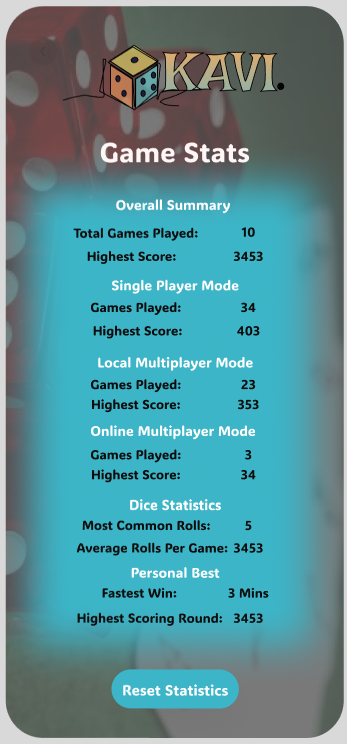
\includegraphics[scale=0.45]{img/stats.png}
        \caption{Design page 2}
        \label{fig:figma_design2}
    \end{subfigure}
    \caption{Initial UI designs and prototypes created in Figma}
    \label{fig:figma_designs}
\end{figure}

\subsection{Design Process}
The application's design process began with creating detailed wireframes and prototypes in Figma. The designs underwent several iterations based on user feedback and technical constraints, evolving into the final implementation. Figure~\ref{fig:figma_designs} shows some of the initial design concepts and their evolution \cite{bib:kavifigma}.

Various existing solutions and design tools inspired the design of the application, one of which stood out was the board screen design was inspired by a dice application project by binaryshrey \cite{bib:binaryshrey}. This repository provided a minimalistic and intuitive approach to dice roll applications, which influenced the layout and functionality of the board screen in this project.

\subsection{Model Training}

The dice detection model was developed using Roboflow's platform, which streamlined the entire process from dataset creation to deployment. The training dataset, depicted in Figure~\ref{fig:roboflow_dataset}, consisted of carefully annotated dice images across various conditions, ensuring robust detection performance in real-world scenarios.

\begin{figure}[h]
    \centering
    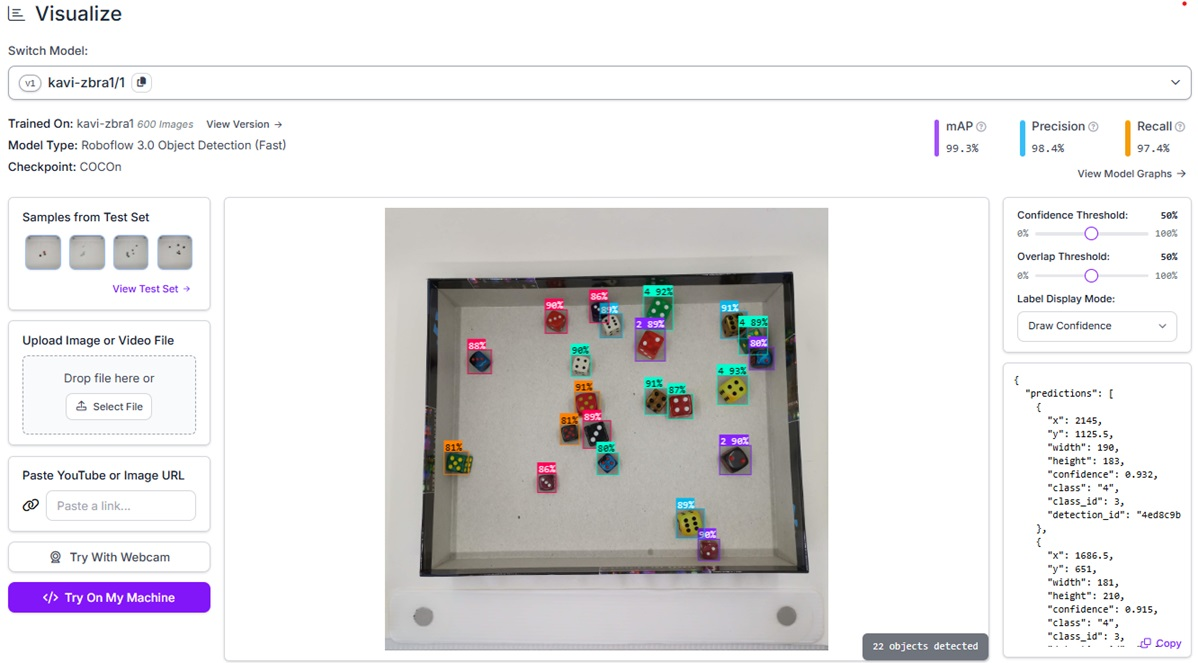
\includegraphics[width=\textwidth]{img/roboflow_dataset.jpg}
    \caption{Roboflow dataset management interface showing dice image annotations}
    \label{fig:roboflow_dataset}
\end{figure}

Roboflow facilitated data augmentation and preprocessing, which enhanced the dataset's diversity. The model training and optimization phases were crucial for achieving high accuracy, while the deployment and API integration ensured seamless real-time inference capabilities.

\subsection{Project Timeline}

The project was implemented from November 2024 to January 2025, following a structured timeline as shown in Figure~\ref{fig:gantt}. The development process was organized into major phases, including planning, design, core development, AI integration, and testing, with regular milestones to track progress.

\begin{figure}[h]
    \centering
    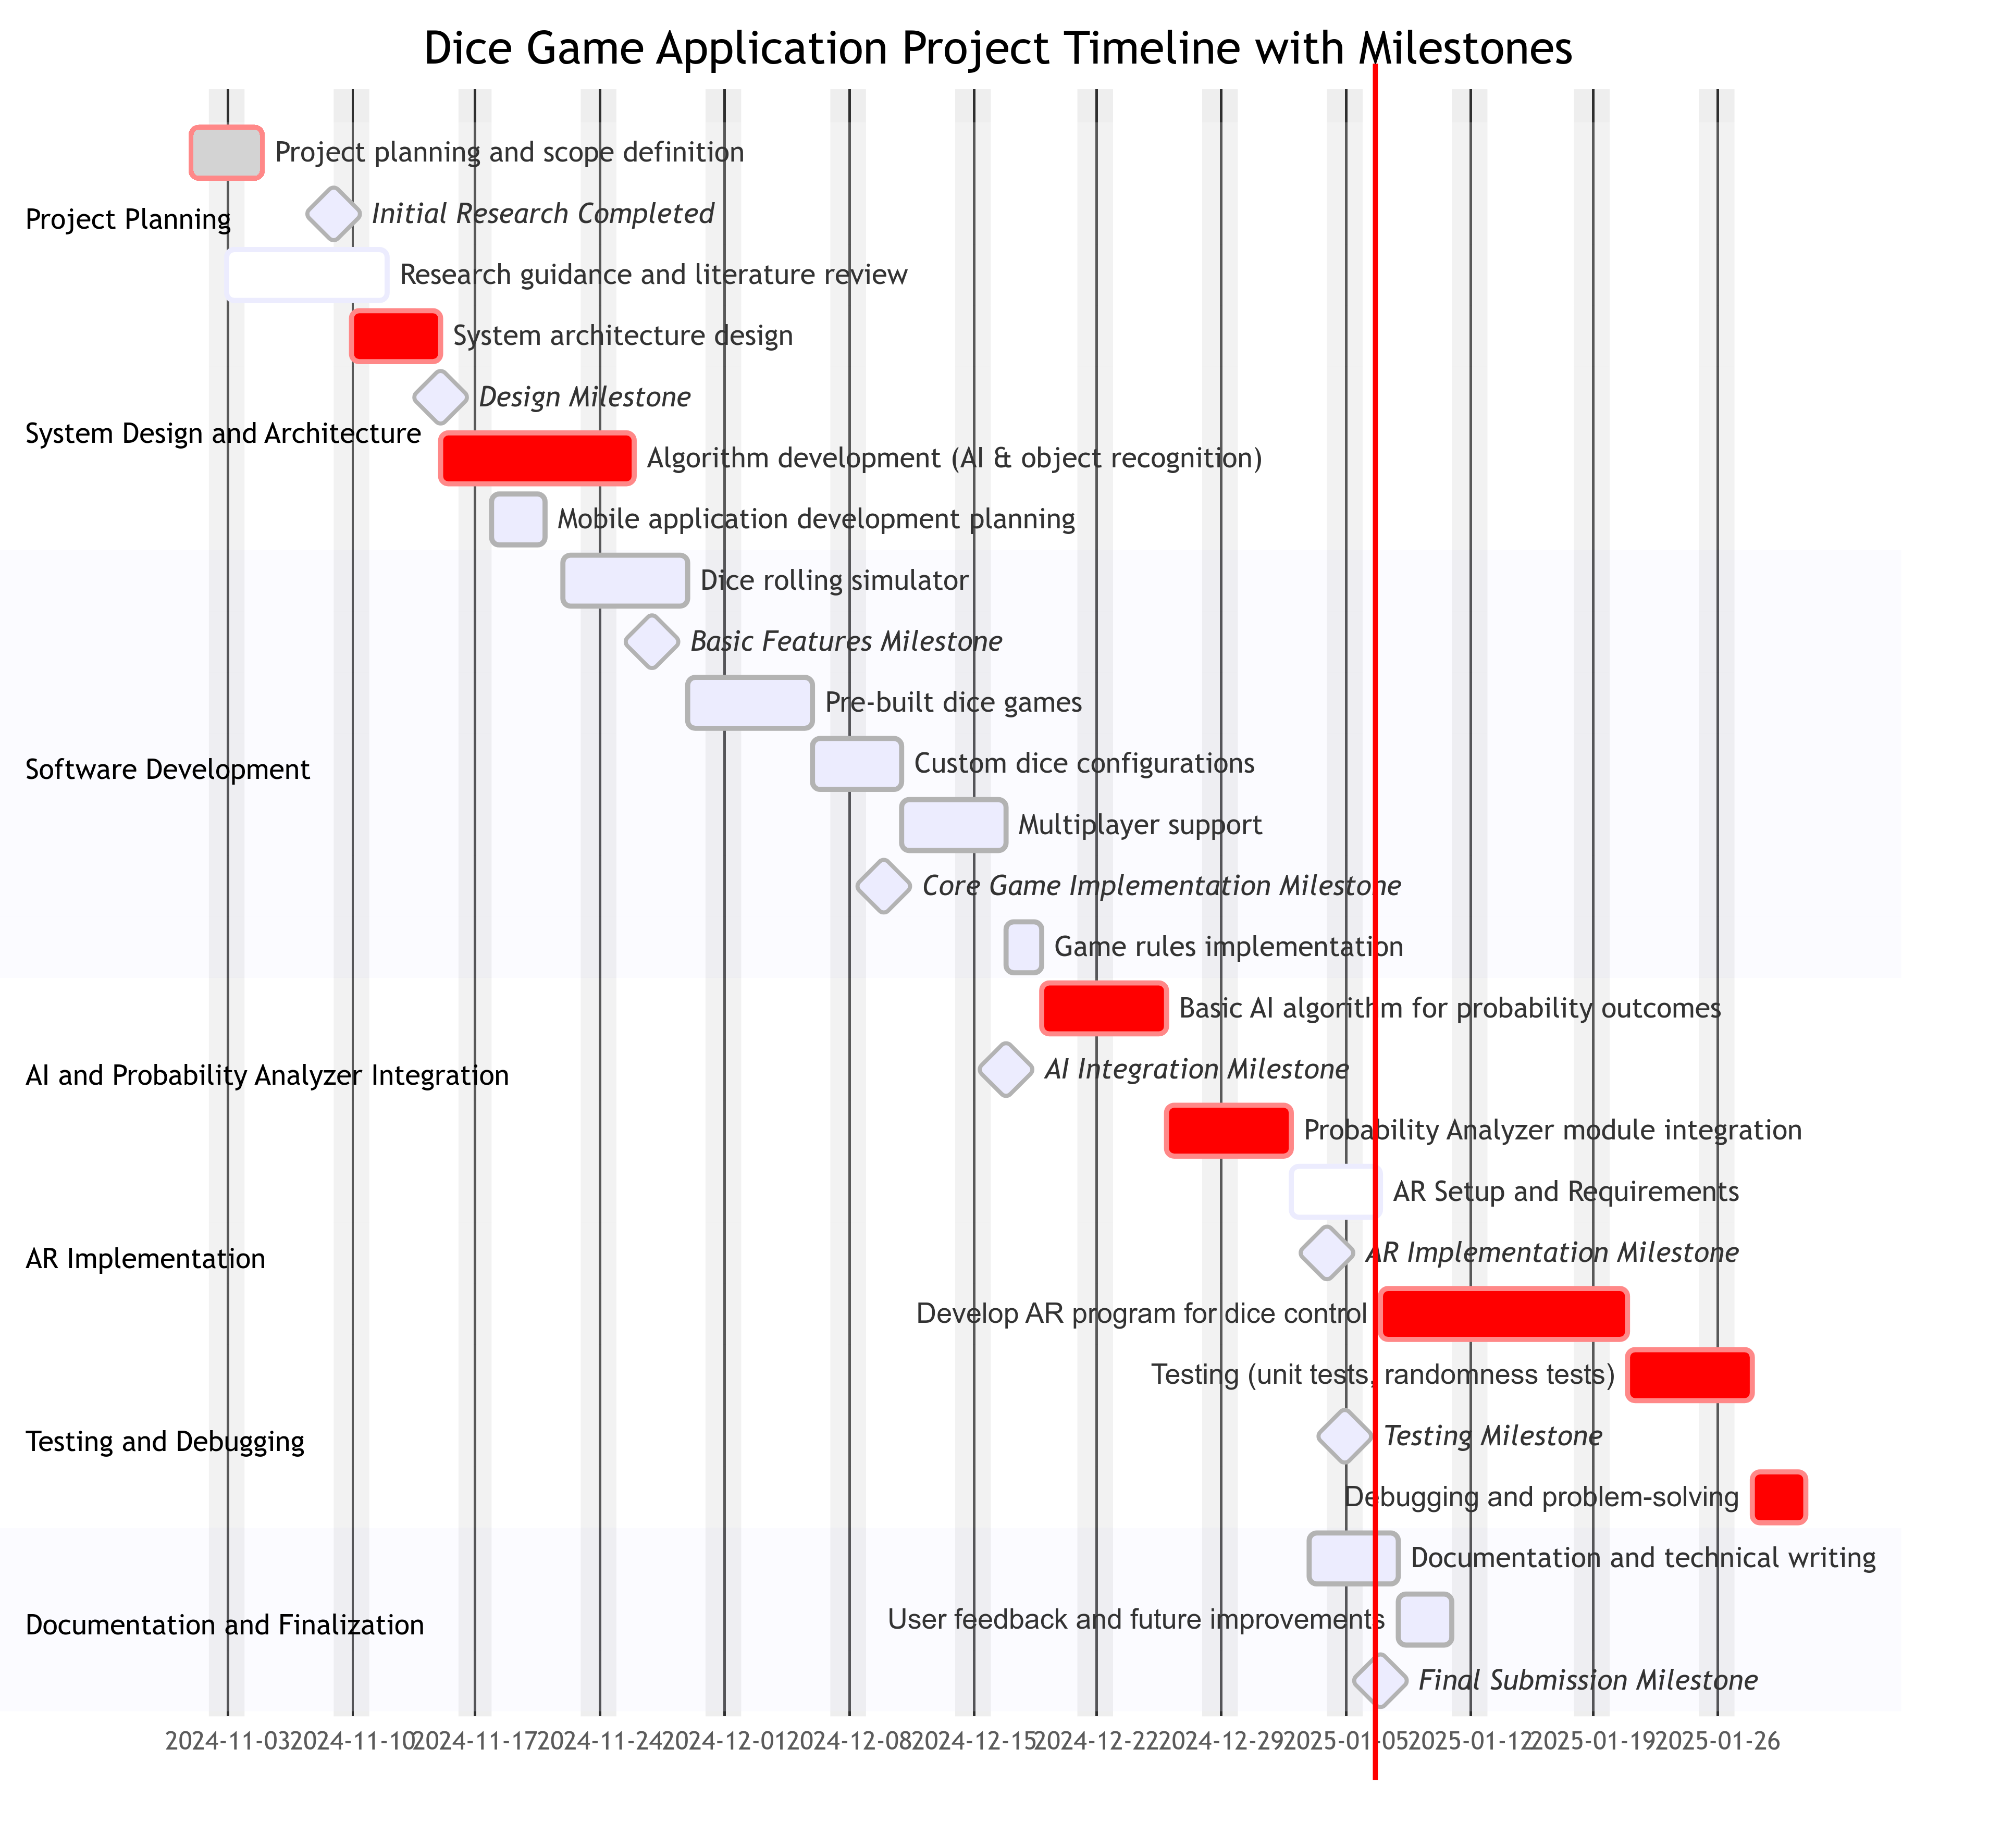
\includegraphics[width=\textwidth]{img/gantt_chart.png}
    \caption{Project Gantt chart showing development phases and milestones}
    \label{fig:gantt}
\end{figure}

This structured approach allowed for continuous improvement and adaptation to changing requirements, ensuring a high-quality application. While some initially planned features like AR implementation were identified as future enhancements, the focus remained on delivering a robust core game experience with AI capabilities.

\chapter{External Specification}

This chapter provides a detailed overview of the external specifications for the application. It outlines the specific requirements for its operation and the installation procedures necessary for a straightforward setup. Additionally, it includes key information to improve user understanding and ensure the application fulfils its intended purpose effectively.

\section{Hardware and Software Requirements}
\subsection{Hardware Requirements}
\begin{itemize}
    \item Android smartphone with Android 11.0 (API level 30) or higher.
    \item Camera with support for CameraX.
     \item Minimum 2GB RAM for standard use of the application, or 3GB RAM for optimal performance on devices with lower memory and processing power.
    \item Internet connection for the dice recognition module; the other parts of the app do not require internet and will work otherwise.
    \item At least 100MB of free storage space.
    \item Processor: ARM-based processor supporting Neon instruction set.
\end{itemize}

\subsection{Software Requirements}
To build the application, the following software is required:
\begin{itemize}
    \item Android Studio Giraffe (2023.1.1) or later.
    \item Kotlin 2.0.21
    \item Gradle 8.10.2 and the corresponding Android Gradle Plugin (e.g. 8.1.2).
    \item CameraX library version: 1.4.0.
\end{itemize}

\section{Installation Procedure}
For installing the application, the following procedure is required:

\subsection{APK Download}
\begin{enumerate}
    \item Download the Release APK from the project's repository at \href{https://github.com/Mayokun-Sofowora/kavi/releases/download/v1.0.0/app-release.apk}{GitHub Releases Page}.
    \item Enable installation from unknown sources in the device's settings. Note that installing apps from unknown sources has security implications; please proceed with caution.
    \item Open the APK file and follow the on-screen instructions.
\end{enumerate}

\subsection{Building with Android Studio}
To install the application for debugging purposes, follow these procedures:
\begin{enumerate}
    \item \textbf{Clone the Repository}: Start by cloning the project repository from GitHub.
    \begin{verbatim}
        git clone https://github.com/Mayokun-Sofowora/kavi.git
    \end{verbatim}
    \item \textbf{Open in Android Studio}: Launch Android Studio and open the cloned project.
    \item \textbf{Sync Gradle Dependencies}: Allow Android Studio to sync the Gradle dependencies automatically.
    \item \textbf{Run on Device/Emulator}: Connect an Android device or start an emulator with a minimum SDK of 30, then run the application.
\end{enumerate}

In addition to the instructions provided, be sure that:
\begin{itemize}
    \item  A debug build variant is selected in Android Studio.
    \item USB debugging is enabled in the device's settings.
    \item You connect an Android device via USB or use an emulator.
    \item  You select the appropriate run configuration in Android Studio.
\end{itemize}

\section{Types of Users}
\begin{itemize}
    \item \textbf{Regular Users}: Play dice games, use image recognition features, and adjust settings.
    \item \textbf{Developers/Testers}: Access debugging logs, experimental features, and perform system administration tasks.
\end{itemize}

\section{User Manual}
\label{sec:user_manual}

\subsection{Navigating the App}

When starting the game, users are welcomed with a splash screen that displays the application's logo in figure~\ref{fig:splash_screen}. After a short moment, the main menu is shown in figure~\ref{fig:main_menu}. The main menu provides navigation options to access the different features of the application.
\begin{figure}[h]
    \centering
    \begin{subfigure}[b]{0.27\textwidth}
        \centering
        \fbox{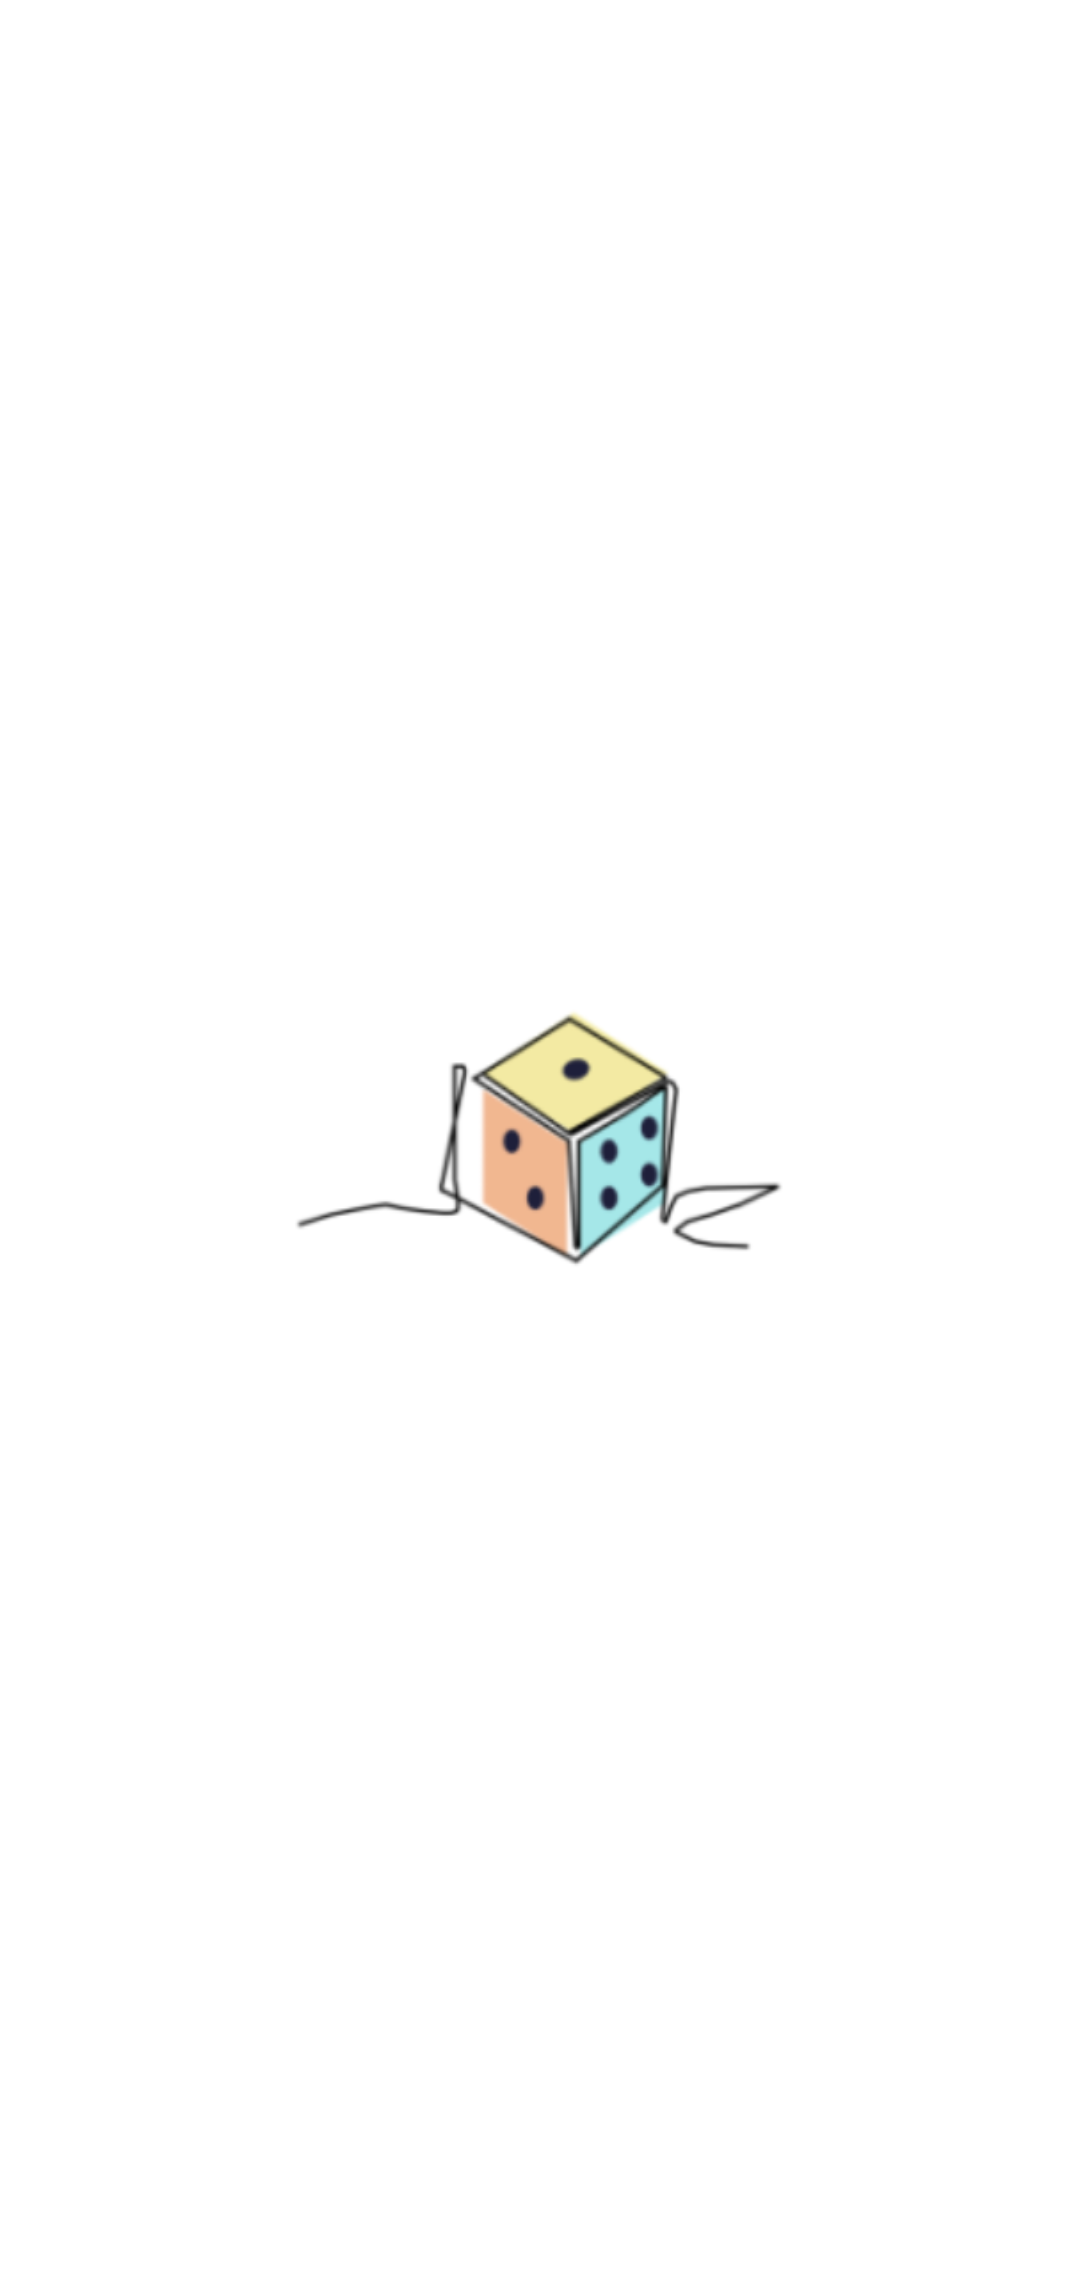
\includegraphics[width=\textwidth]{img/splash screen.png}}
        \caption{The Splash Screen}
        \label{fig:splash_screen}
    \end{subfigure}
    \hspace{1em}
    \begin{subfigure}[b]{0.27\textwidth}
        \centering
        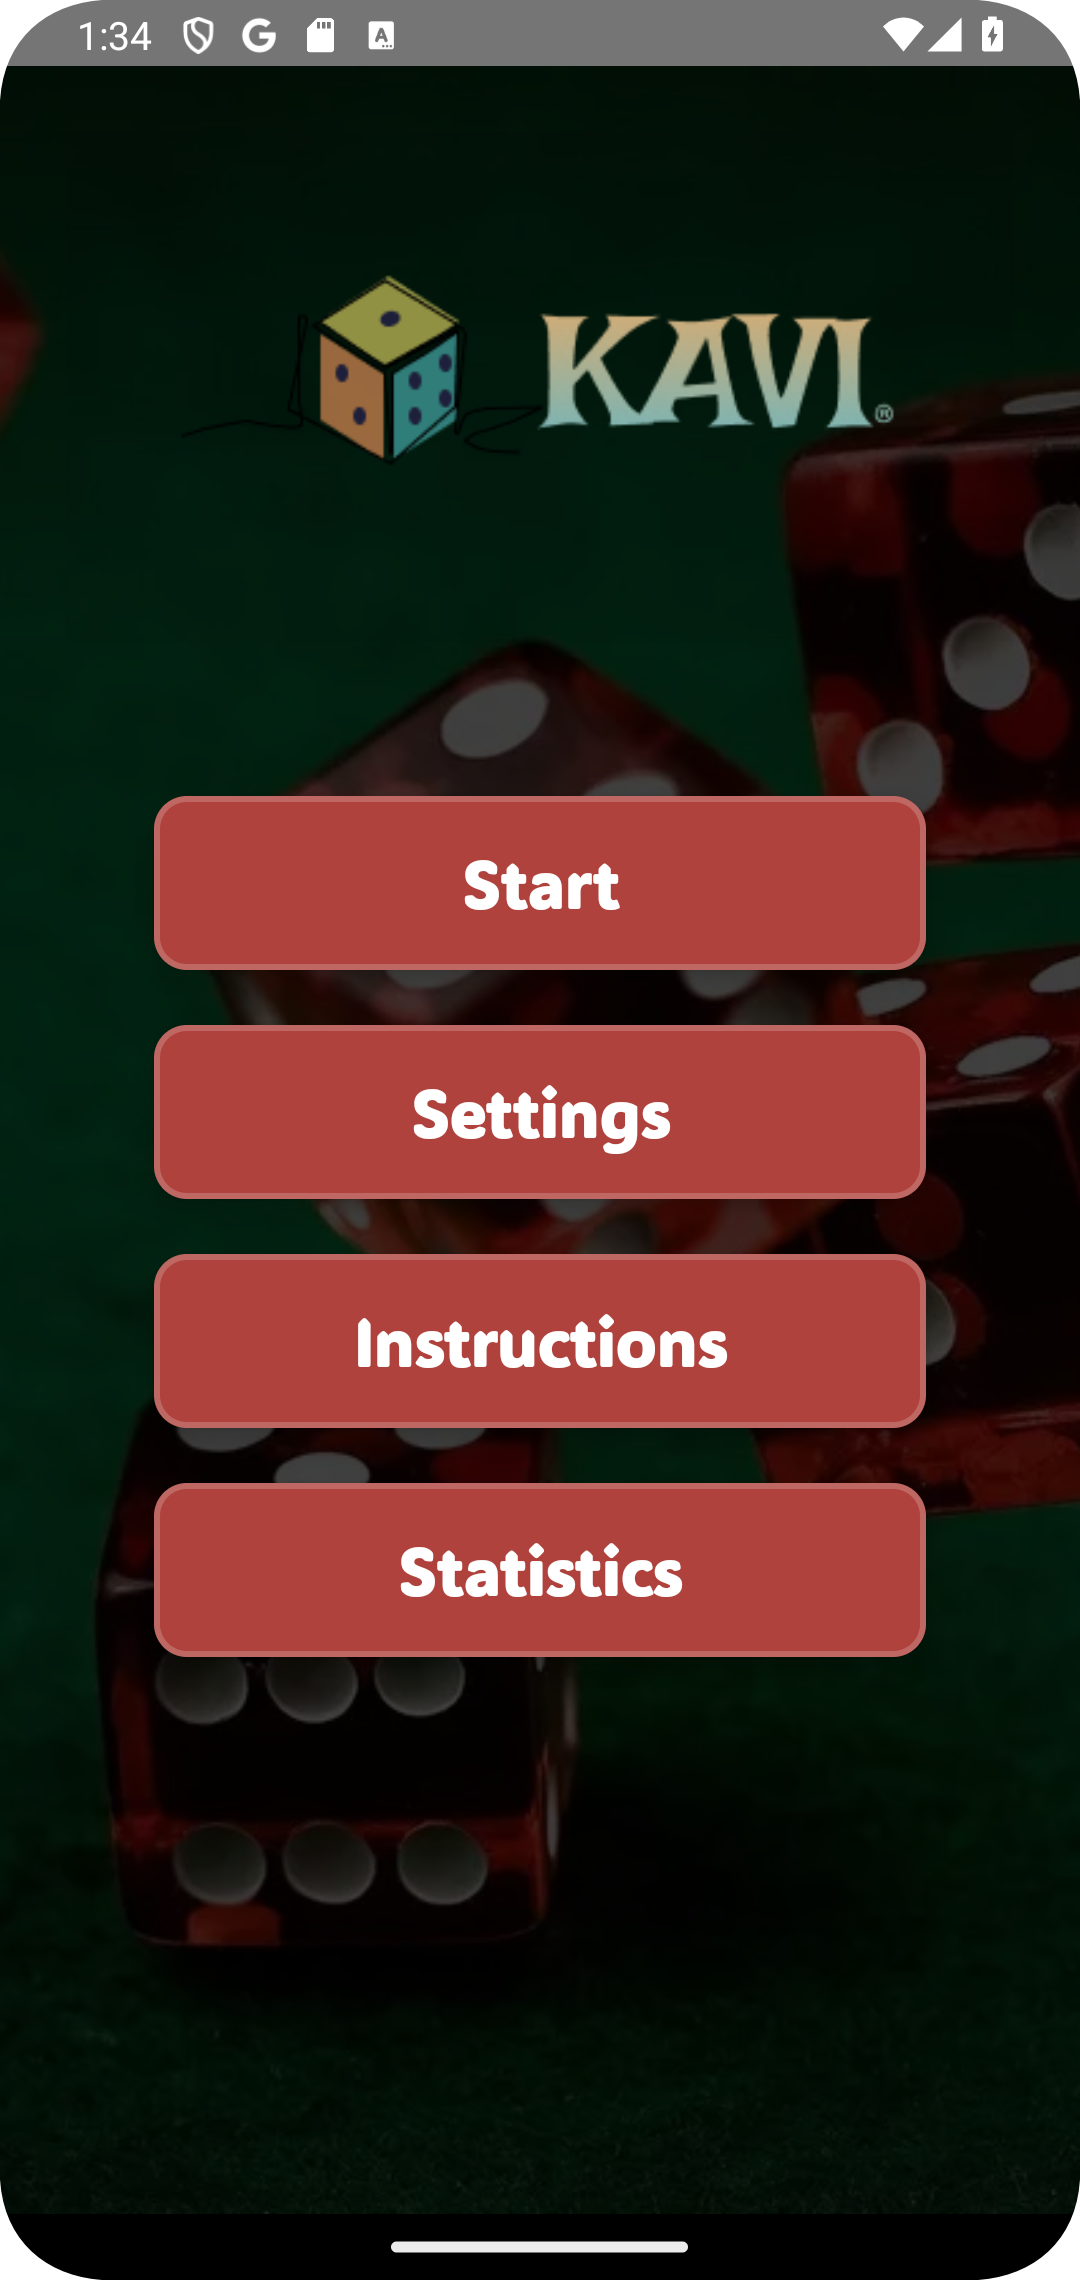
\includegraphics[width=\textwidth]{img/main menu.png}
        \caption{The Main Menu}
        \label{fig:main_menu}
    \end{subfigure}
    \caption{Screens displayed when starting the game.}
    \label{fig:starting_game}
\end{figure}

\subsection{Game Interface}

The interface allows users to navigate to different sections of the application, such as the classic boards to play the classic dice games or the virtual screen to use the image recognition feature. The figure~\ref{fig:interface_mode} shows the navigation options available.

\begin{figure}[h]
    \centering
    \begin{subfigure}[b]{0.27\textwidth}
        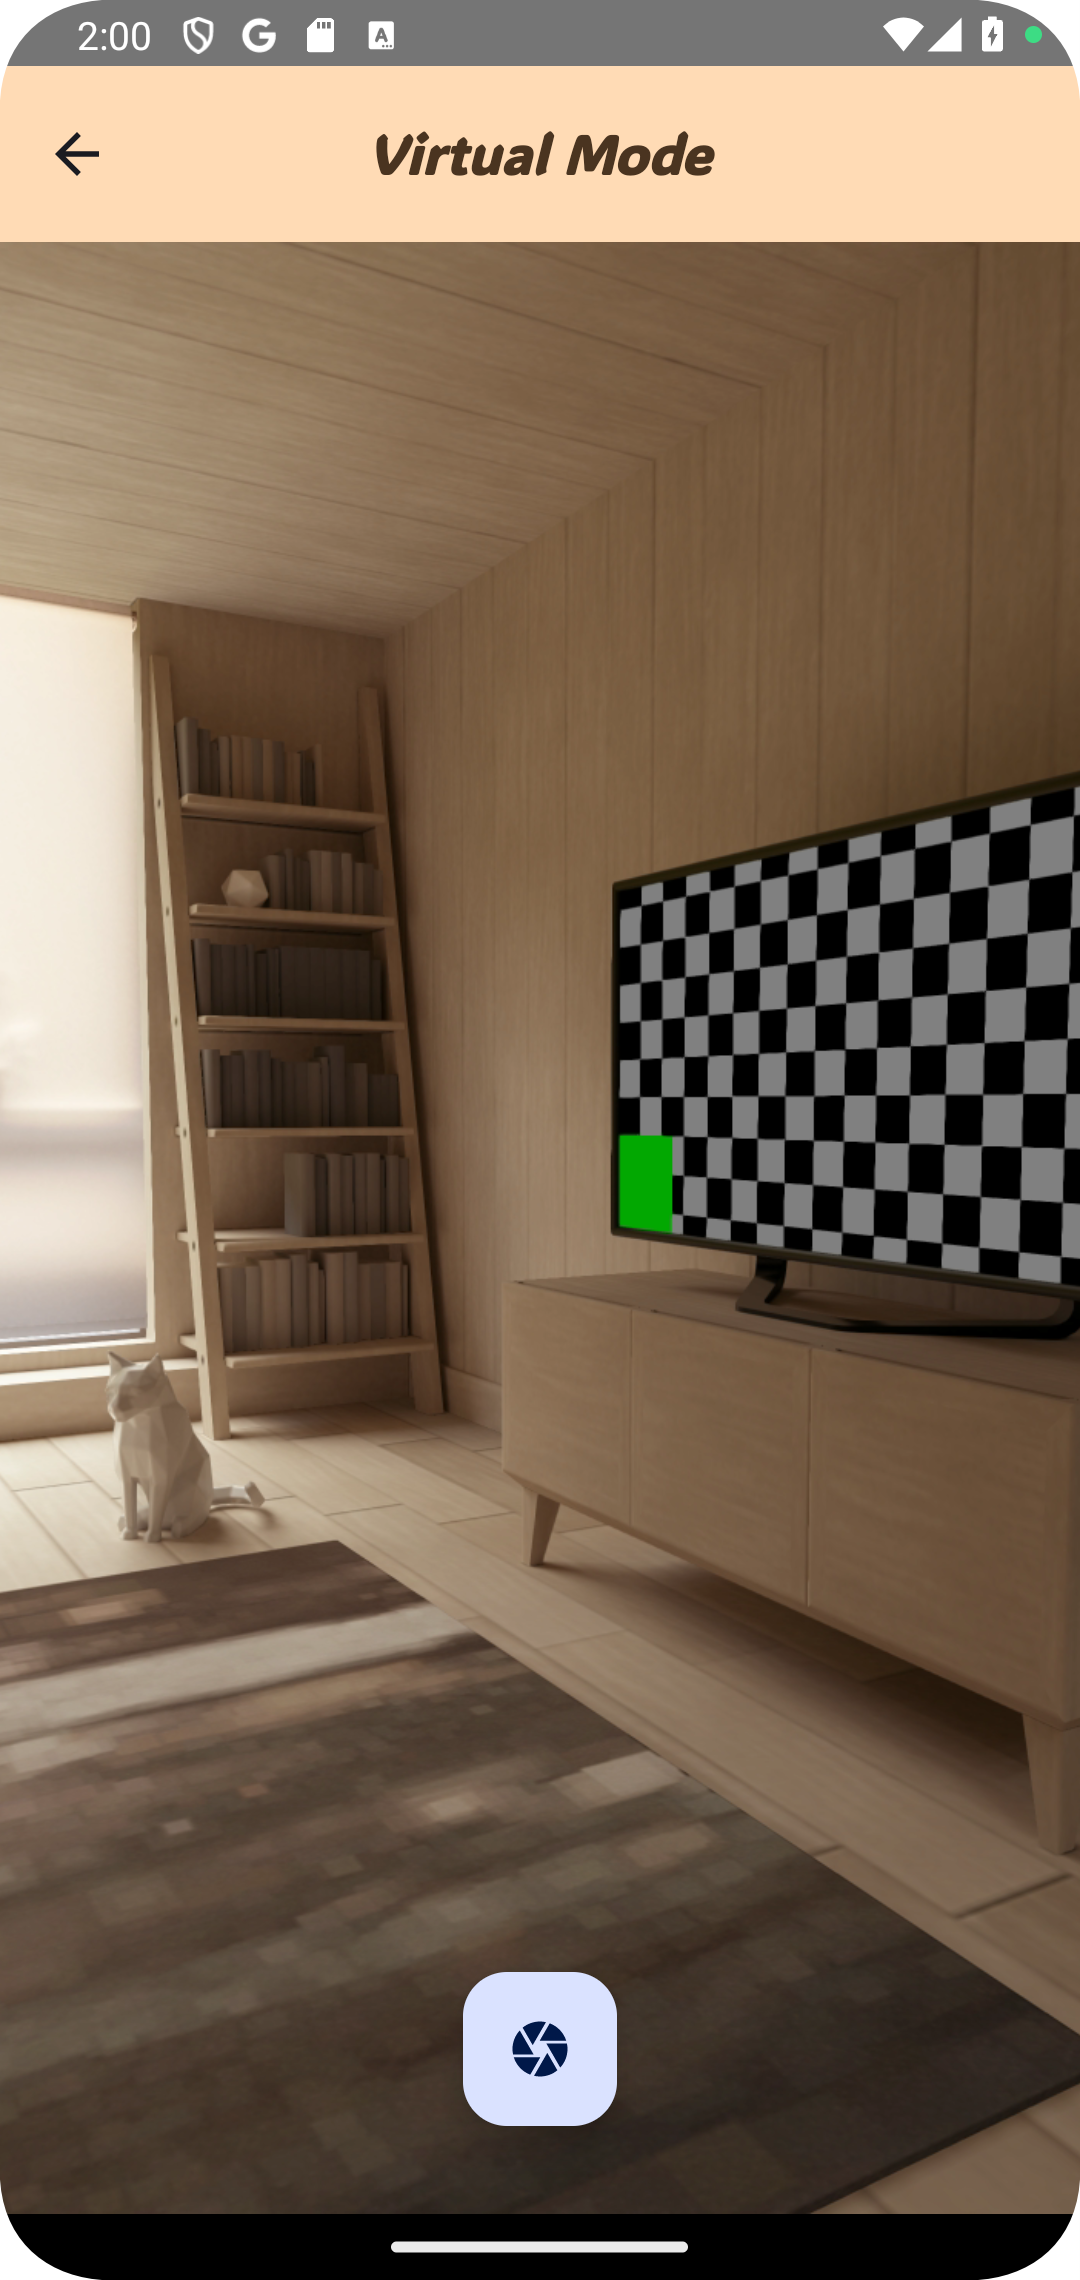
\includegraphics[width=\textwidth]{img/virtual mode.png}
        \caption{Virtual Mode}
        \label{fig:virtual_mode}
    \end{subfigure}
    \hfill
    \begin{subfigure}[b]{0.27\textwidth}
        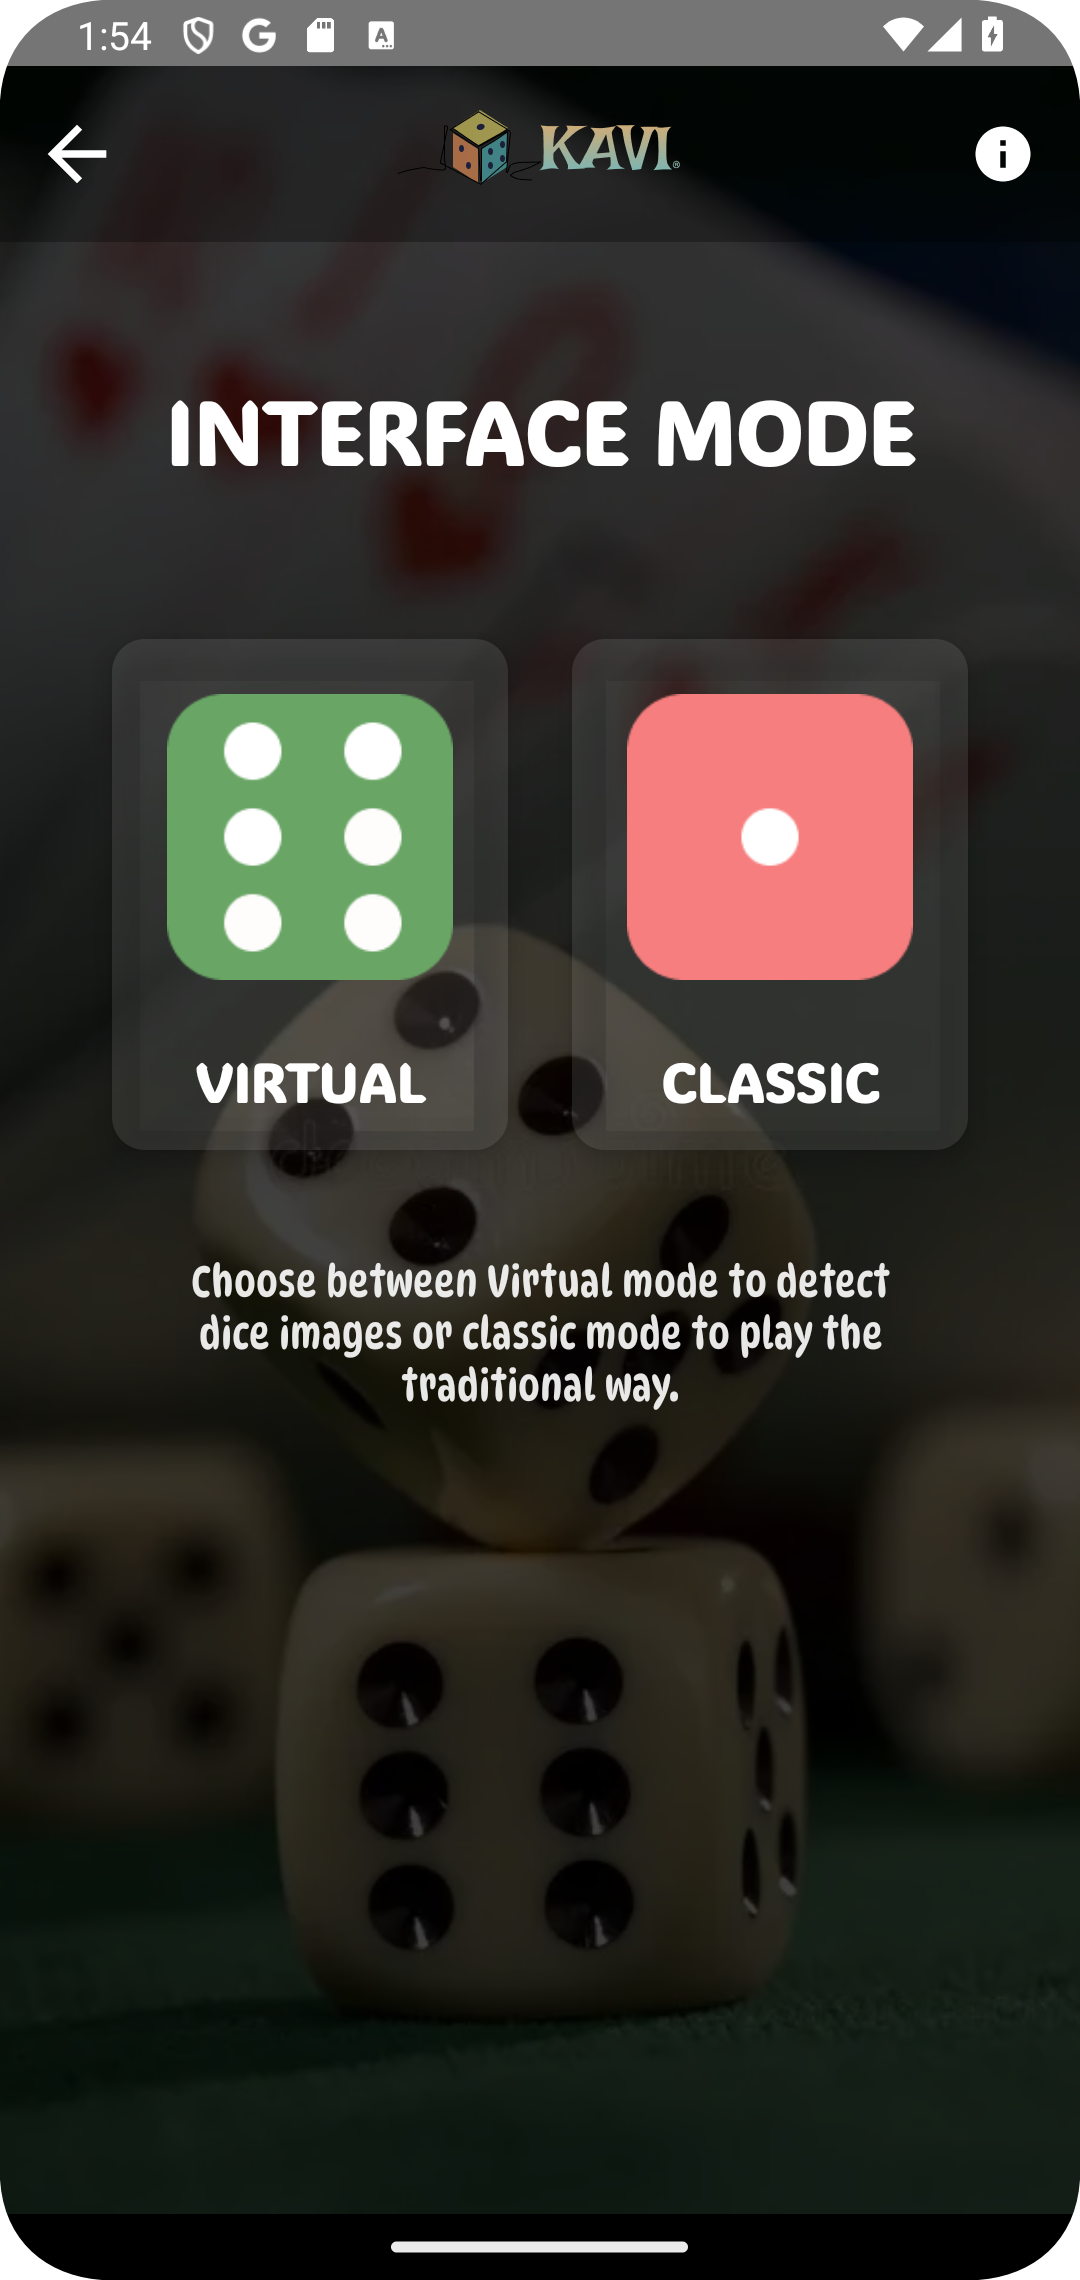
\includegraphics[width=\textwidth]{img/interface mode.png}
        \caption{The Start Screen}
        \label{fig:start_screen}
    \end{subfigure}
    \hfill
    \begin{subfigure}[b]{0.27\textwidth}
        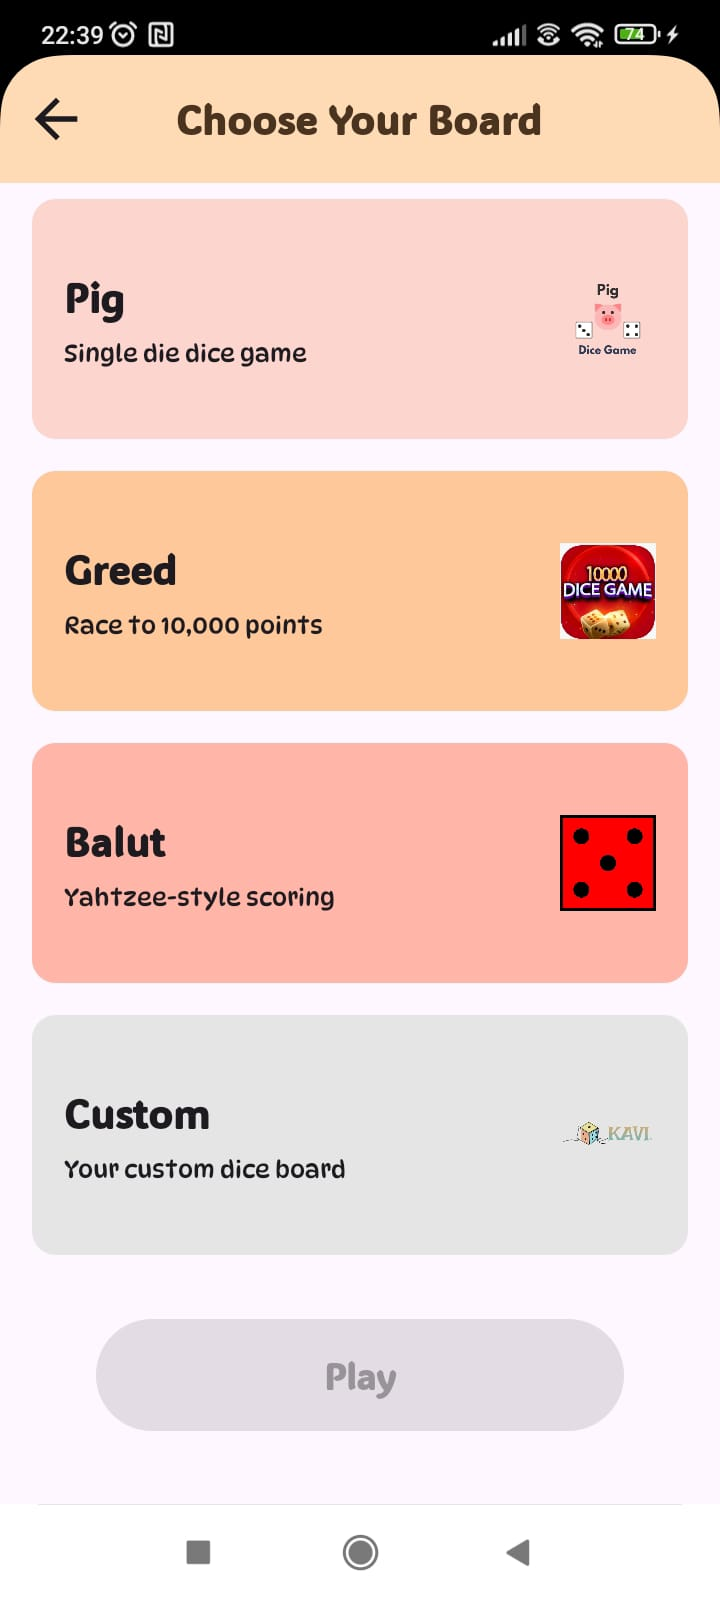
\includegraphics[width=\textwidth]{img/classic boards.jpg}
        \caption{Classic Mode}
        \label{fig:board_screen}
    \end{subfigure}
\caption{The Games main interfaces.}
\label{fig:interface_mode}
\end{figure}

\subsection{Classic Boards}

The application offers a diverse set of game boards, each designed for a distinct dice game experience. These games range from simple "press-your-luck" scenarios to more strategic challenges that require planning and risk management. The primary games offered are \textit{Pig}, \textit{Greed}, and \textit{Balut}. Additionally, the application includes a custom board where users can define their own game rules and scoring mechanisms, and also select the number of dice used in the game. The figure~\ref{fig:board_screen} shows the classic boards available in the application.

\begin{figure}[h]
    \centering
    \begin{subfigure}[b]{0.27\textwidth}
        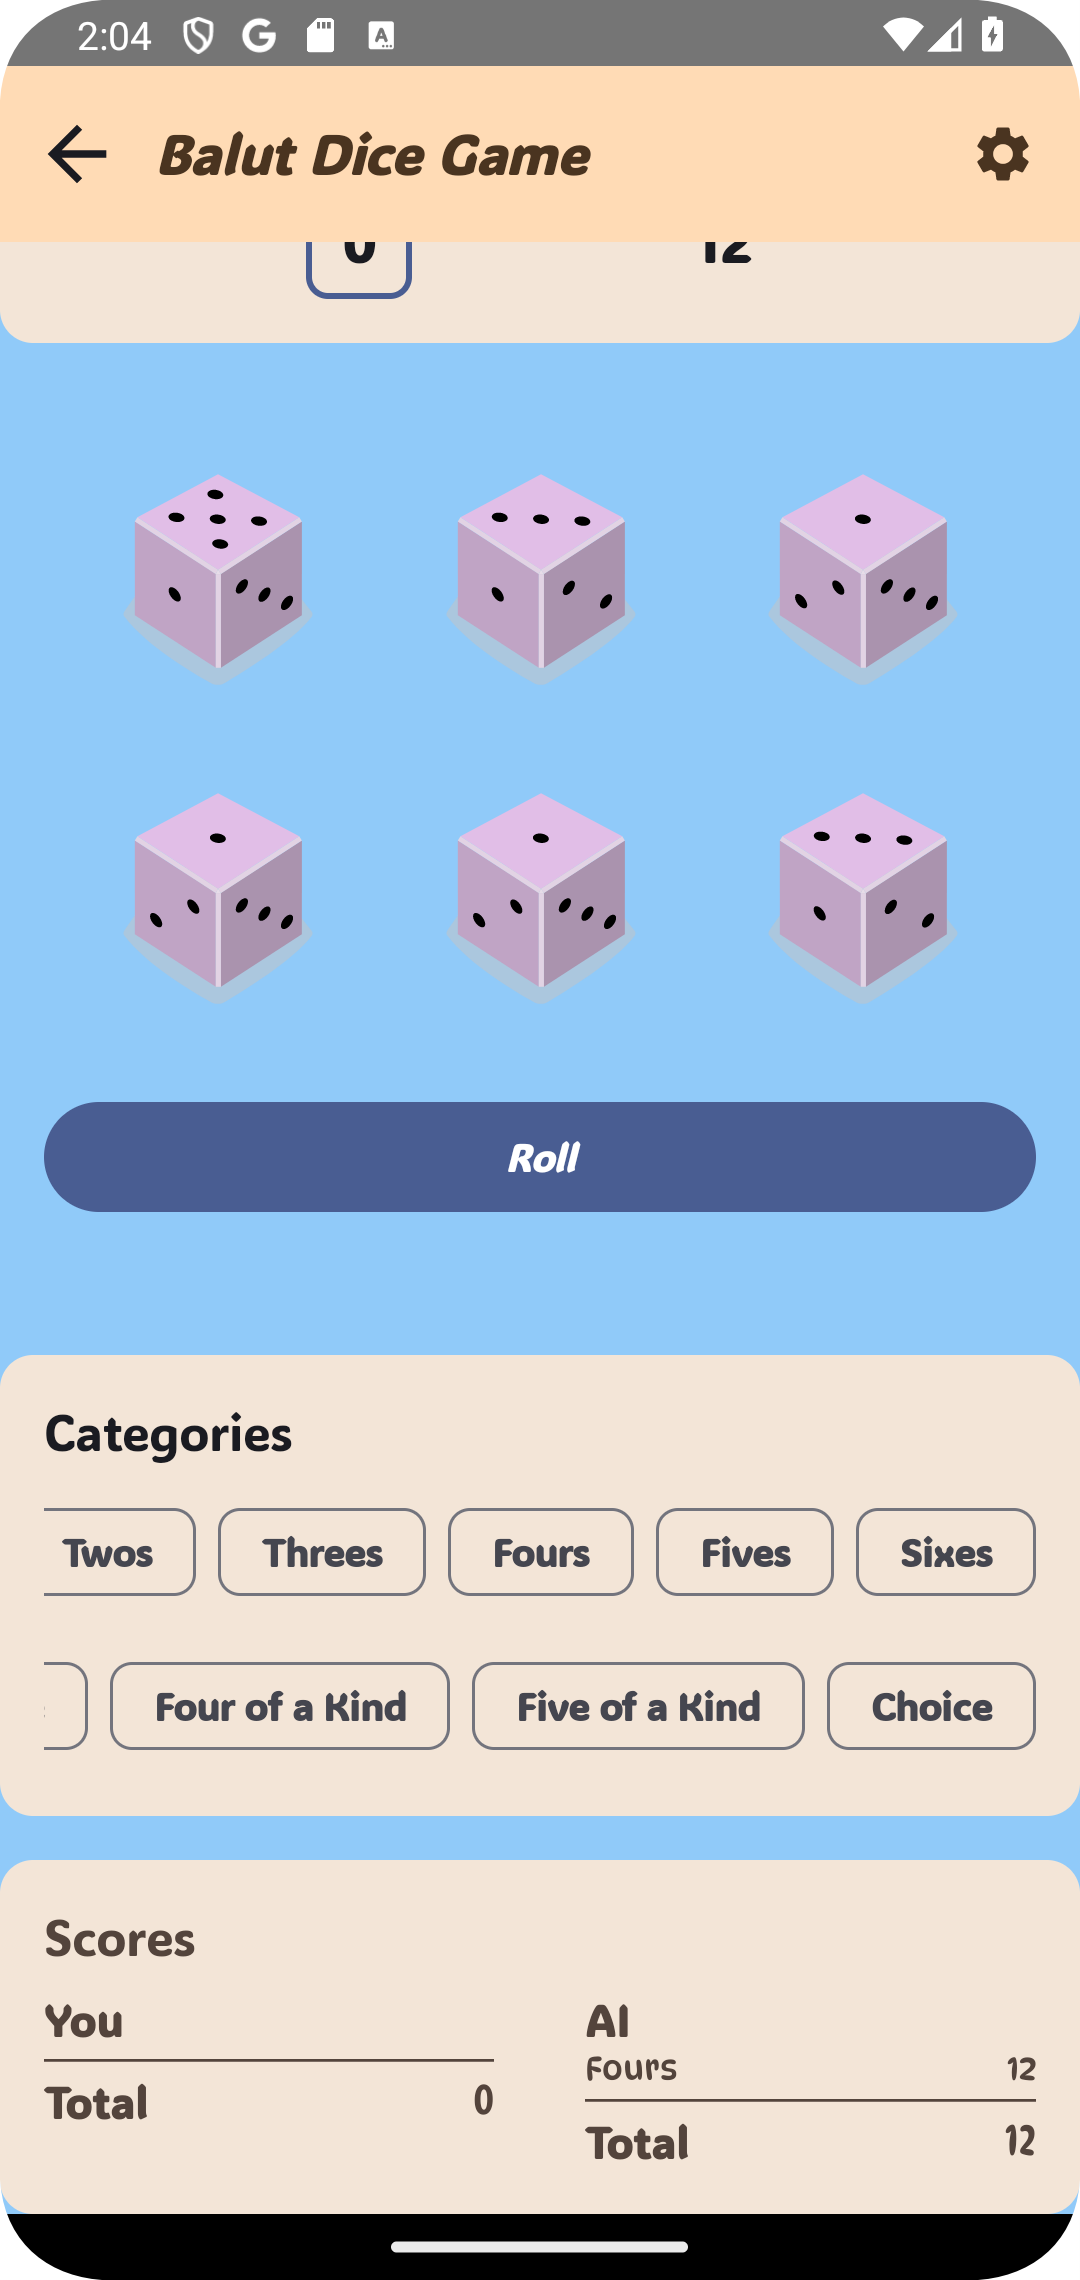
\includegraphics[width=\textwidth]{img/balut board.png}
        \caption{Balut Game Board}
    \end{subfigure}
    \hfill
    \begin{subfigure}[b]{0.27\textwidth}
        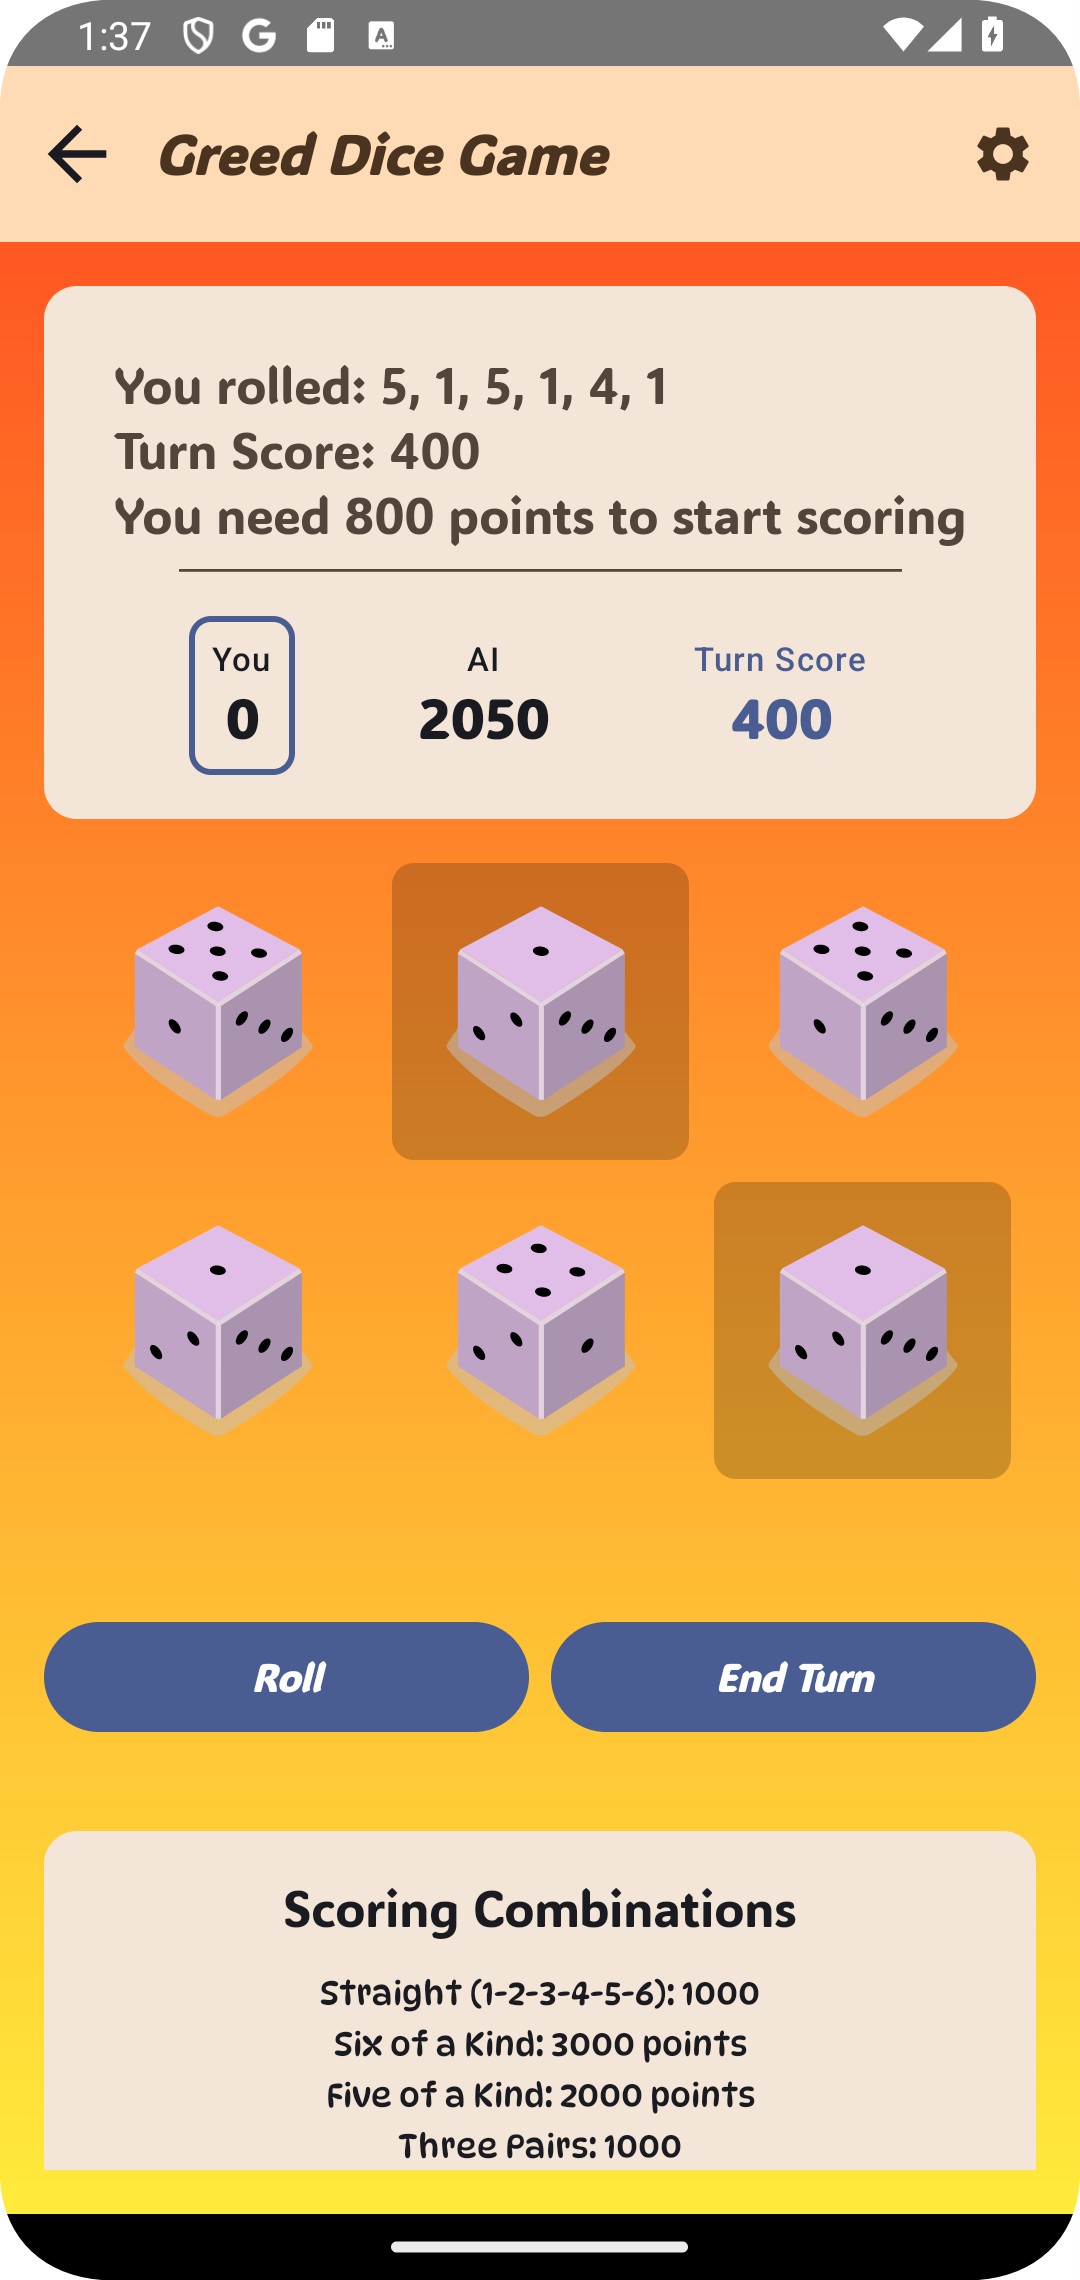
\includegraphics[width=\textwidth]{img/greed board.png}
        \caption{Greed Game Board}
    \end{subfigure}
    \hfill
    \begin{subfigure}[b]{0.27\textwidth}
        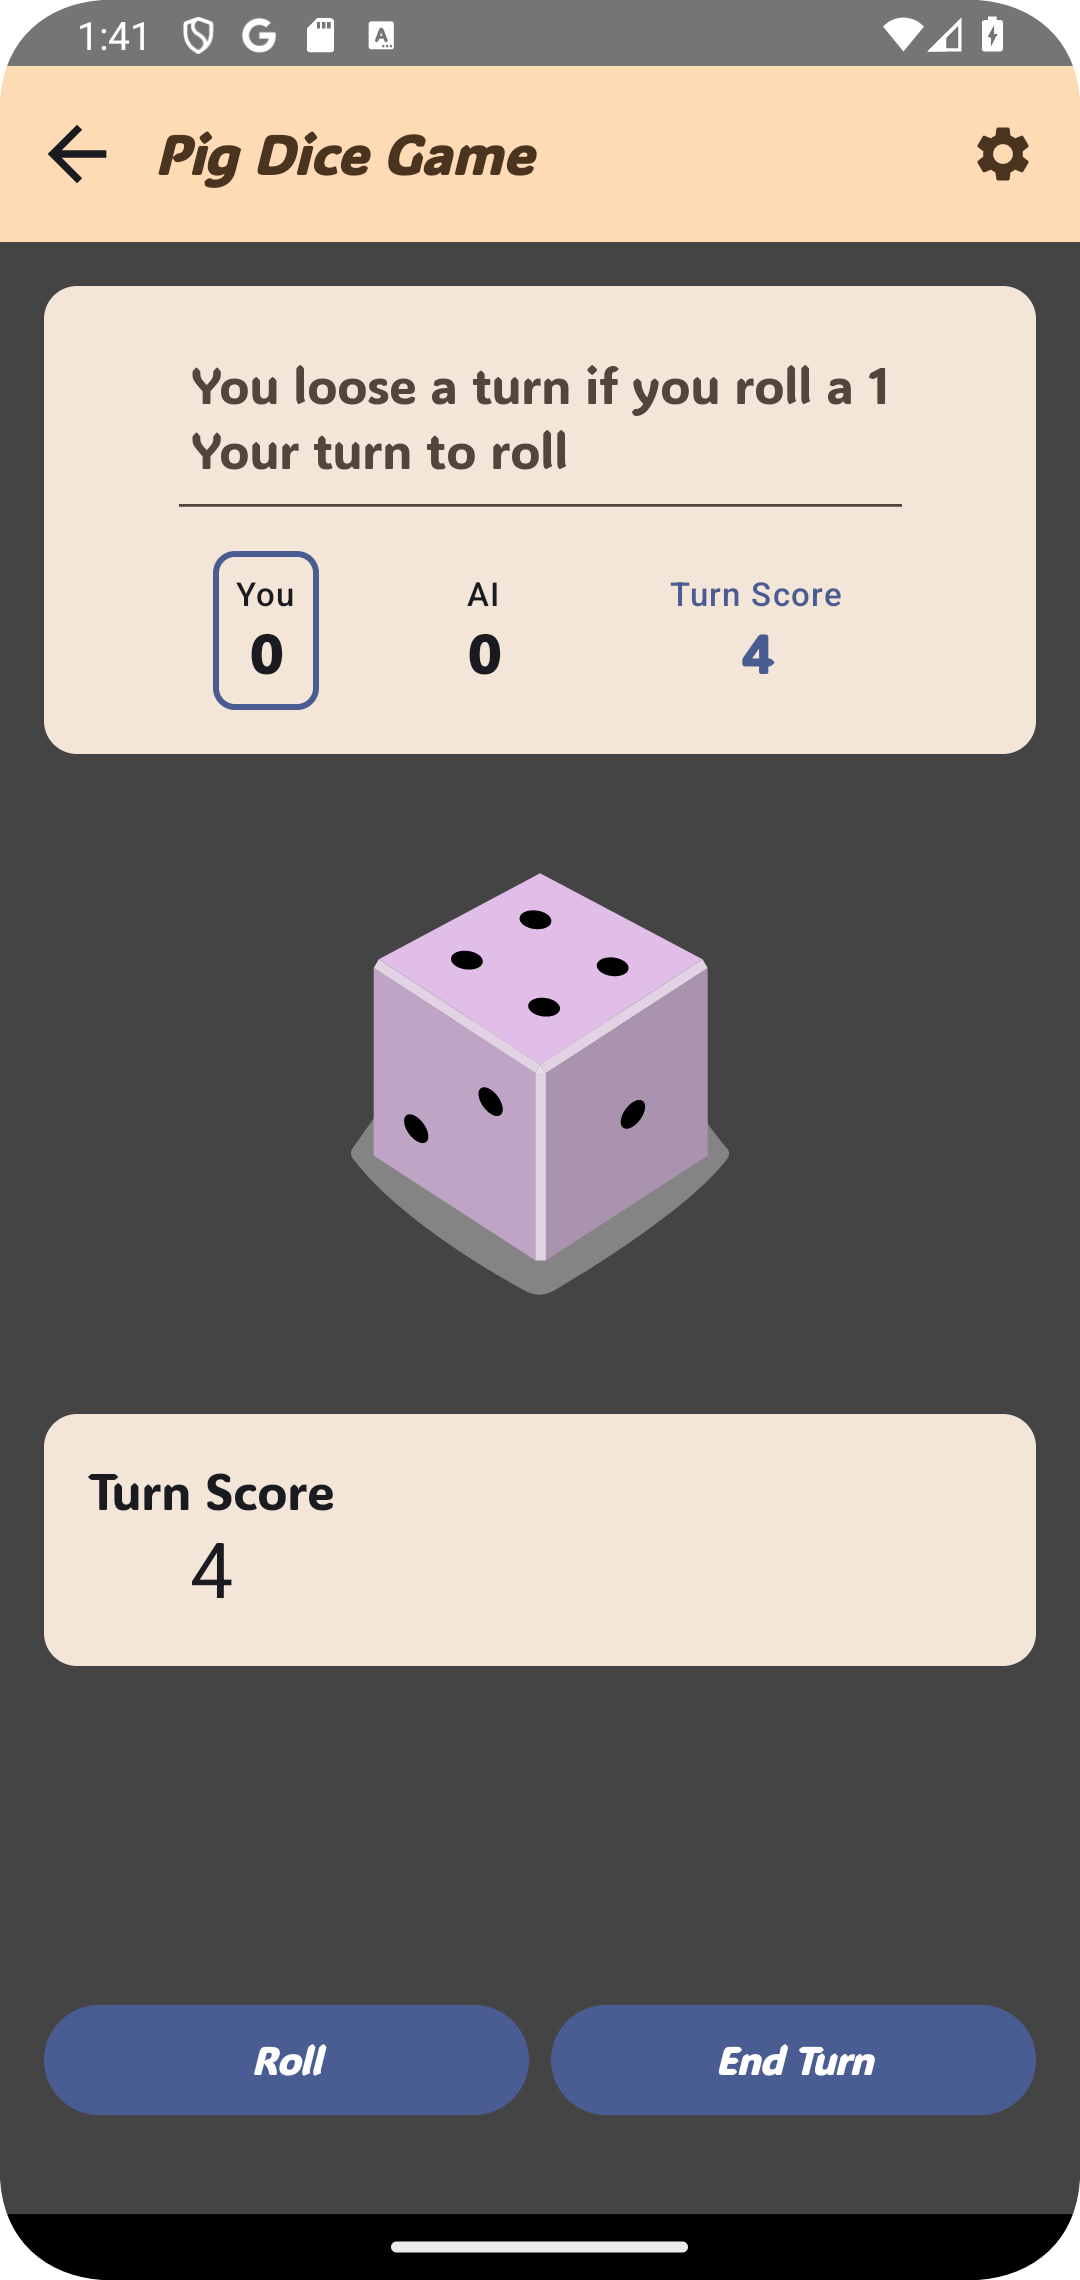
\includegraphics[width=\textwidth]{img/pig board.png}
        \caption{Pig Game Board}
    \end{subfigure}
    \caption{Game Boards in the Application}
\end{figure}

\subsection{Game Objectives}

\subsubsection{Pig: The Risk of the Roll}

Pig is a simple, engaging game of chance and risk. The goal is to be the first player to reach a total of 100 points. During each turn, players roll a single die, accumulating points with each roll. The key aspect of Pig is the ability to "bank" the points you have accumulated in that turn, however, the risk is that if you roll a 1, you lose all the points accumulated during that turn. The challenge lies in choosing when to press your luck for more points and when to play it safe to avoid losing those points.

\subsubsection{Greed: Navigating Scoring Combinations}

Greed is a more complex game that rewards strategic decision-making and risk-taking. Each turn begins with the roll of six dice. After the roll, players get to select which dice they want to keep to accumulate points, based on scoring combinations like straights, sets (e.g., three-of-a-kind, four-of-a-kind), and single 1s and 5s. These combinations vary in their scoring values, meaning that a key aspect of the game is knowing which combinations you should aim for. Unlike Pig, in Greed, players must accumulate at least 800 points in a turn to start banking them. The winner is the first player to reach a total of 10,000 points.

\subsubsection{Balut: Strategic Category Management}

Balut is a game of strategy, similar to Yahtzee. Players have up to three rolls per turn using five dice. The core of Balut is strategically filling the scoring categories, such as sets, straights, full houses, and more. Each category can be used only once, so planning and smart selection of which dice to hold is critical. After all categories are filled, the player with the highest total score wins.

\subsection{Game Controls: Interacting with the Game}

The application provides a user-friendly interface with intuitive controls, allowing players to easily interact with each game and manage their scores. This section talks about the various controls and how they function across different game modes.

\subsubsection{Basic Game Controls (Roll, End Turn)}

The primary way players interact with the games is through the roll button. In games like \textit{Pig} and \textit{Greed}, this button (shown in Figure \ref{fig:control1}) also serves as an "End Turn" button. In these games, tapping the button rolls the dice and also ends the turn after a score is obtained.

\begin{figure}[ht!]
    \centering
    
\includegraphics[width=0.6\textwidth]{img/control1.jpg}
    \caption{Roll and End Turn Button}
    \label{fig:control1}
\end{figure}

\subsubsection{Player Management and Custom Game Setup}

In the custom game board, it is also possible to add players and edit their names (as shown in Figure \ref{fig:control2}). This function can be accessed by tapping a button which allows the player to add and remove player, as well as edit their names. This allows users to set up a new game of their liking.

\begin{figure}[ht!]
    \centering
    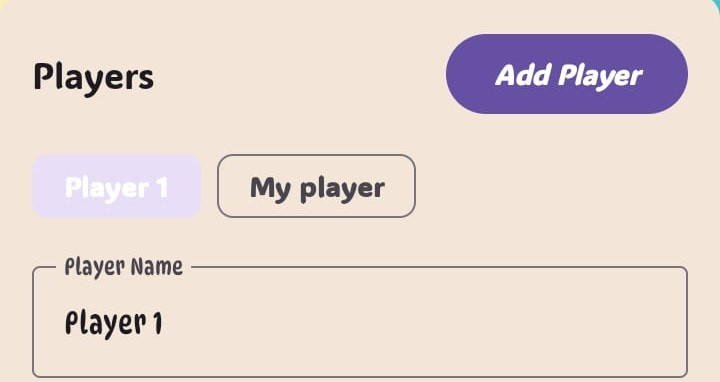
\includegraphics[width=0.6\textwidth]{img/control2.jpg}
    \caption{Player Management and Editing}
    \label{fig:control2}
\end{figure}

\subsubsection{Balut-Specific Controls (Category Selection)}

\textit{Balut} introduces the unique feature of category selection. After rolling the dice, a player can select a category in which to score, shown in Figure \ref{fig:control3}. This allows for a more strategic game, where each category can only be used once.

\begin{figure}[ht!]
    \centering
    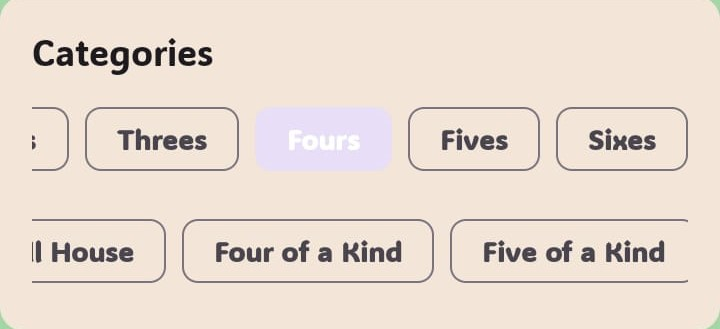
\includegraphics[width=0.6\textwidth]{img/control3.jpg}
    \caption{Balut Category Selection}
    \label{fig:control3}
\end{figure}

\subsubsection{Holding Dice}

In both \textit{Greed} and \textit{Balut}, players can strategically select dice to hold for the next roll. As seen in Figure \ref{fig:control4}, this is done by tapping on the individual dice on the screen. The selected dice will be saved, and can be rolled again in the subsequent roll.

\begin{figure}[ht!]
    \centering
    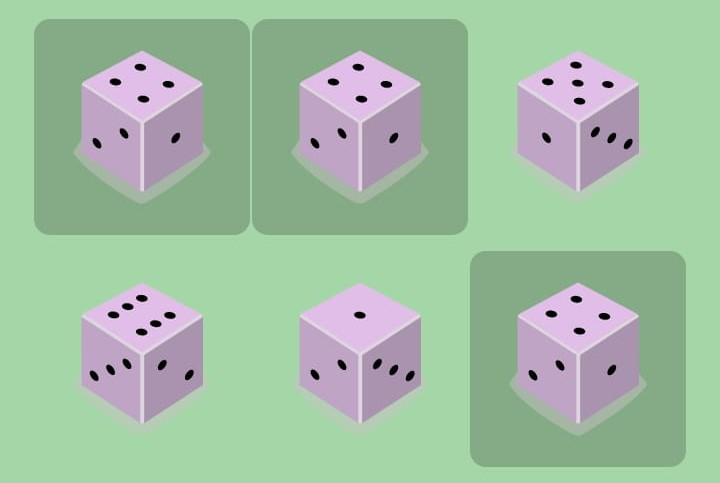
\includegraphics[width=0.6\textwidth]{img/control4.jpg}
    \caption{Selecting Dice to Hold}
     \label{fig:control4}
\end{figure}

\subsubsection{Balut Score Function}

After a category has been selected in \textit{Balut}, the game also provides an additional button which can be tapped to calculate the score and end the turn. As seen in figure \ref{fig:control5}.

\begin{figure}[ht!]
    \centering
    
\includegraphics[width=0.6\textwidth]{img/control5.jpg}
    \caption{Balut Roll and Score Button}
    \label{fig:control5}
\end{figure}

\subsubsection{Custom Board Settings}

The custom board allows players to set the number of dice that will be used for that specific game. In addition, the board name can also be set, as seen in Figure \ref{fig:control6}. This level of customization gives the users control over how the games are played.

\begin{figure}[ht!]
    \centering
    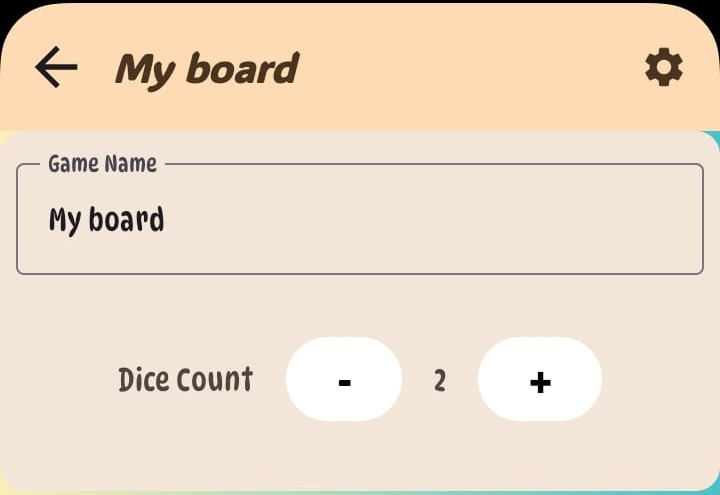
\includegraphics[width=0.6\textwidth]{img/control6.jpg}
    \caption{Custom Board Settings}
    \label{fig:control6}
\end{figure}

\subsubsection{Score Modifiers and Reset}

Figure \ref{fig:control7} shows the score modifiers, which enable users to manually adjust their scores. This feature can also be used to keep track of score in other types of games that might not be covered by this application, or in the custom mode. The feature also contains a reset score button that will reset the score of the game to 0. This can be used to easily restart any game or any other custom use. Additionally, this interface also contains the functionality of adding a note that will be saved as part of the game, which can be used to keep track of important information of the current game.

\begin{figure}[ht!]
    \centering
    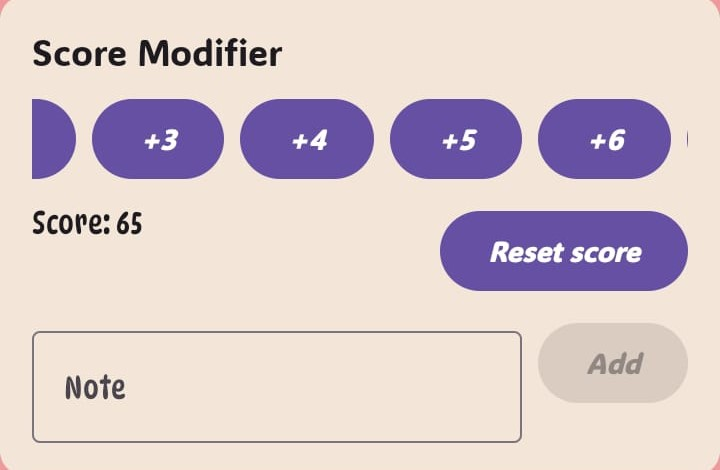
\includegraphics[width=0.6\textwidth]{img/control7.jpg}
    \caption{Score Modifiers and Reset}
     \label{fig:control7}
\end{figure}

\subsection{Instruction}

The instructions screen provides users with detailed guidance on how to play the game. It includes rules, tips, and strategies to enhance the gaming experience. The instructions screen is illustrated in Figure~\ref{fig:instructions_screen}.

\subsection{Settings}
The settings screen, on the other hand, allows users to customize their gaming experience, such as enabling vibration, the shake-to-roll function, and board color customization. The settings screen is shown in Figure~\ref{fig:settings_screen}.

\begin{figure}[h]
    \centering
    \begin{subfigure}[b]{0.27\textwidth}
        \centering
        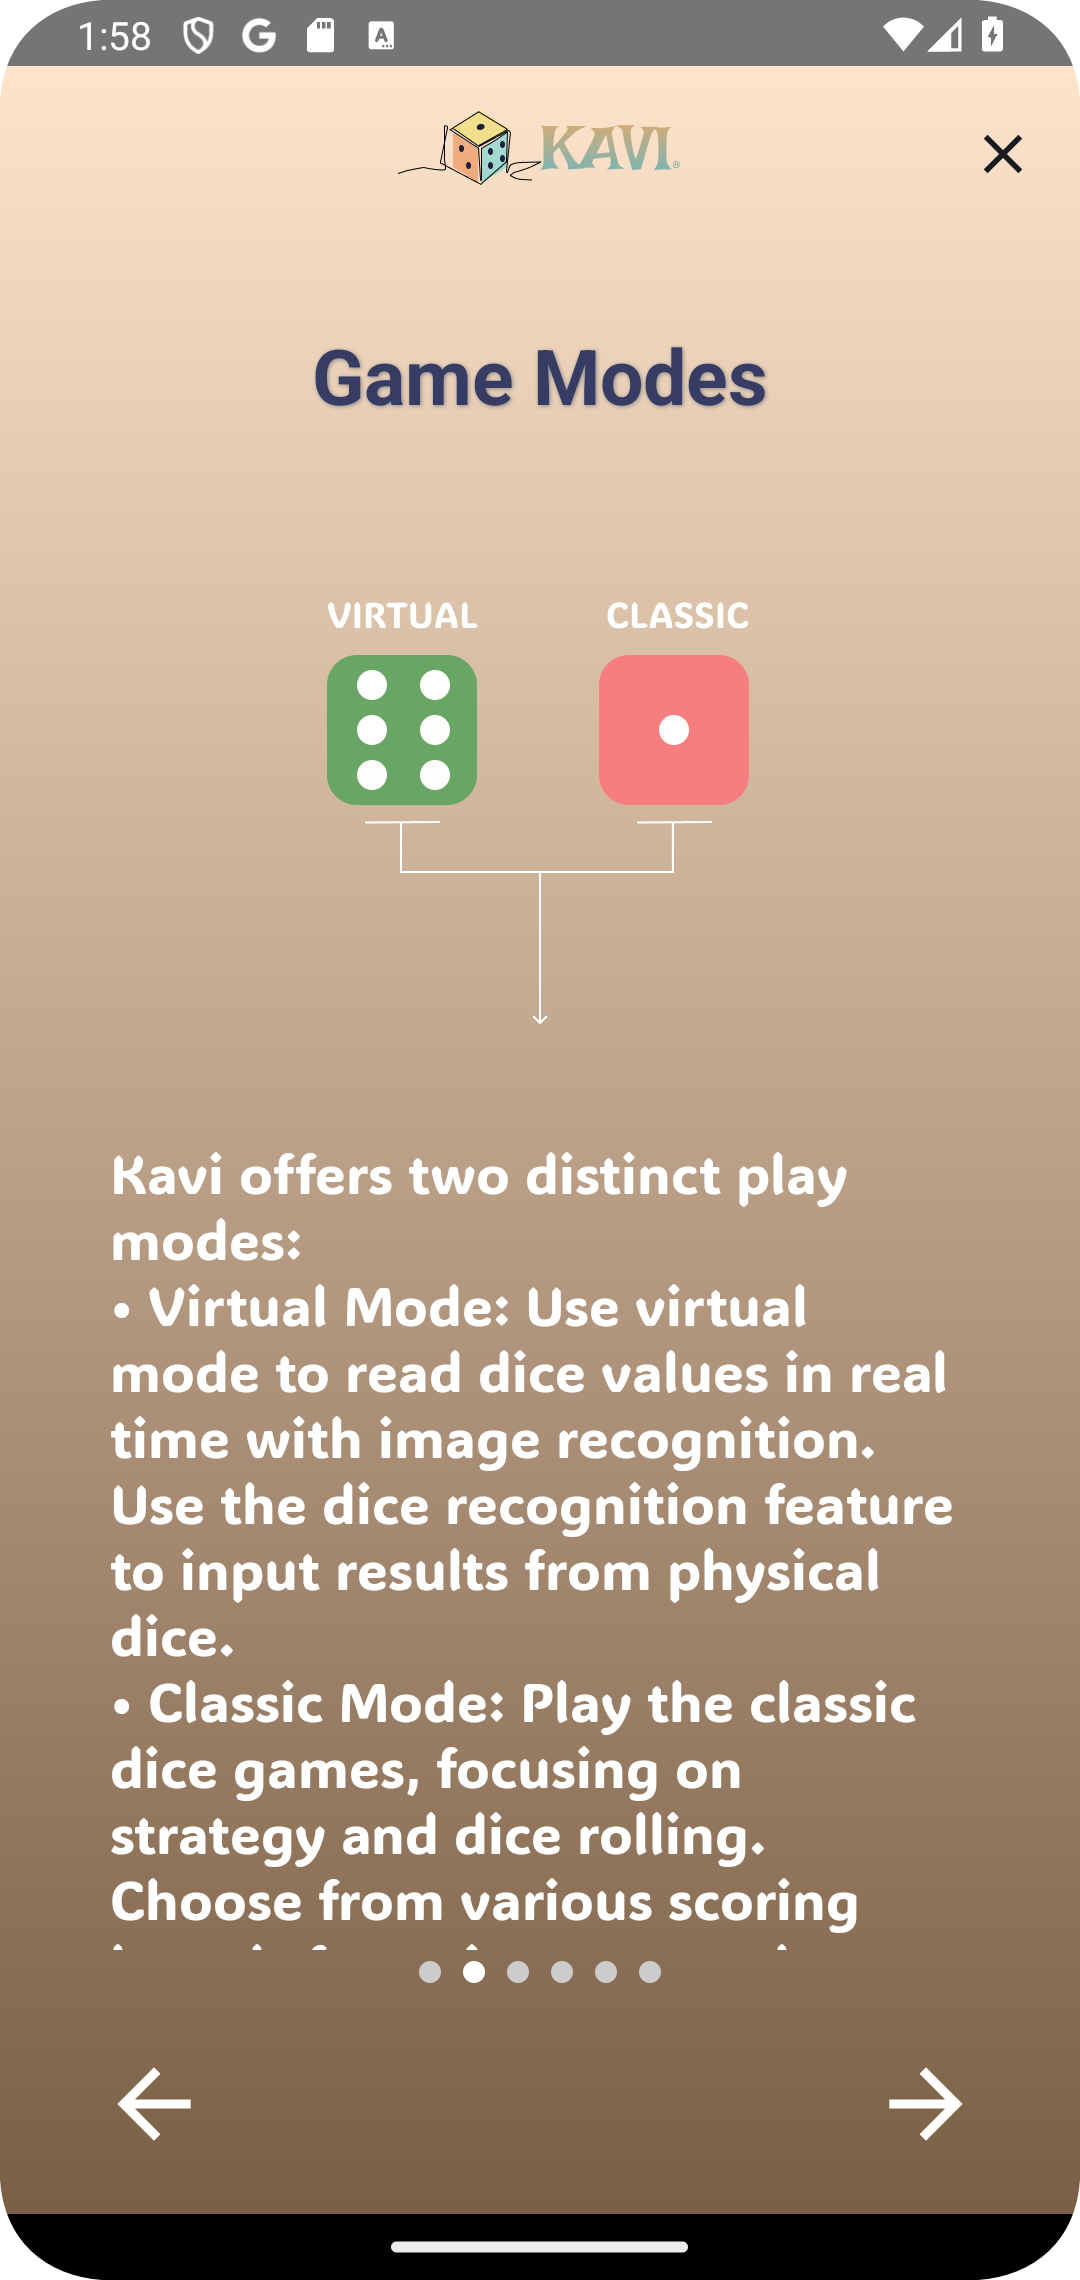
\includegraphics[width=\textwidth]{img/instructions screen.png}
        \caption{Instructions Screen}
        \label{fig:instructions_screen}
    \end{subfigure}
    \hspace{.5em}
    \begin{subfigure}[b]{0.27\textwidth}
        \centering
        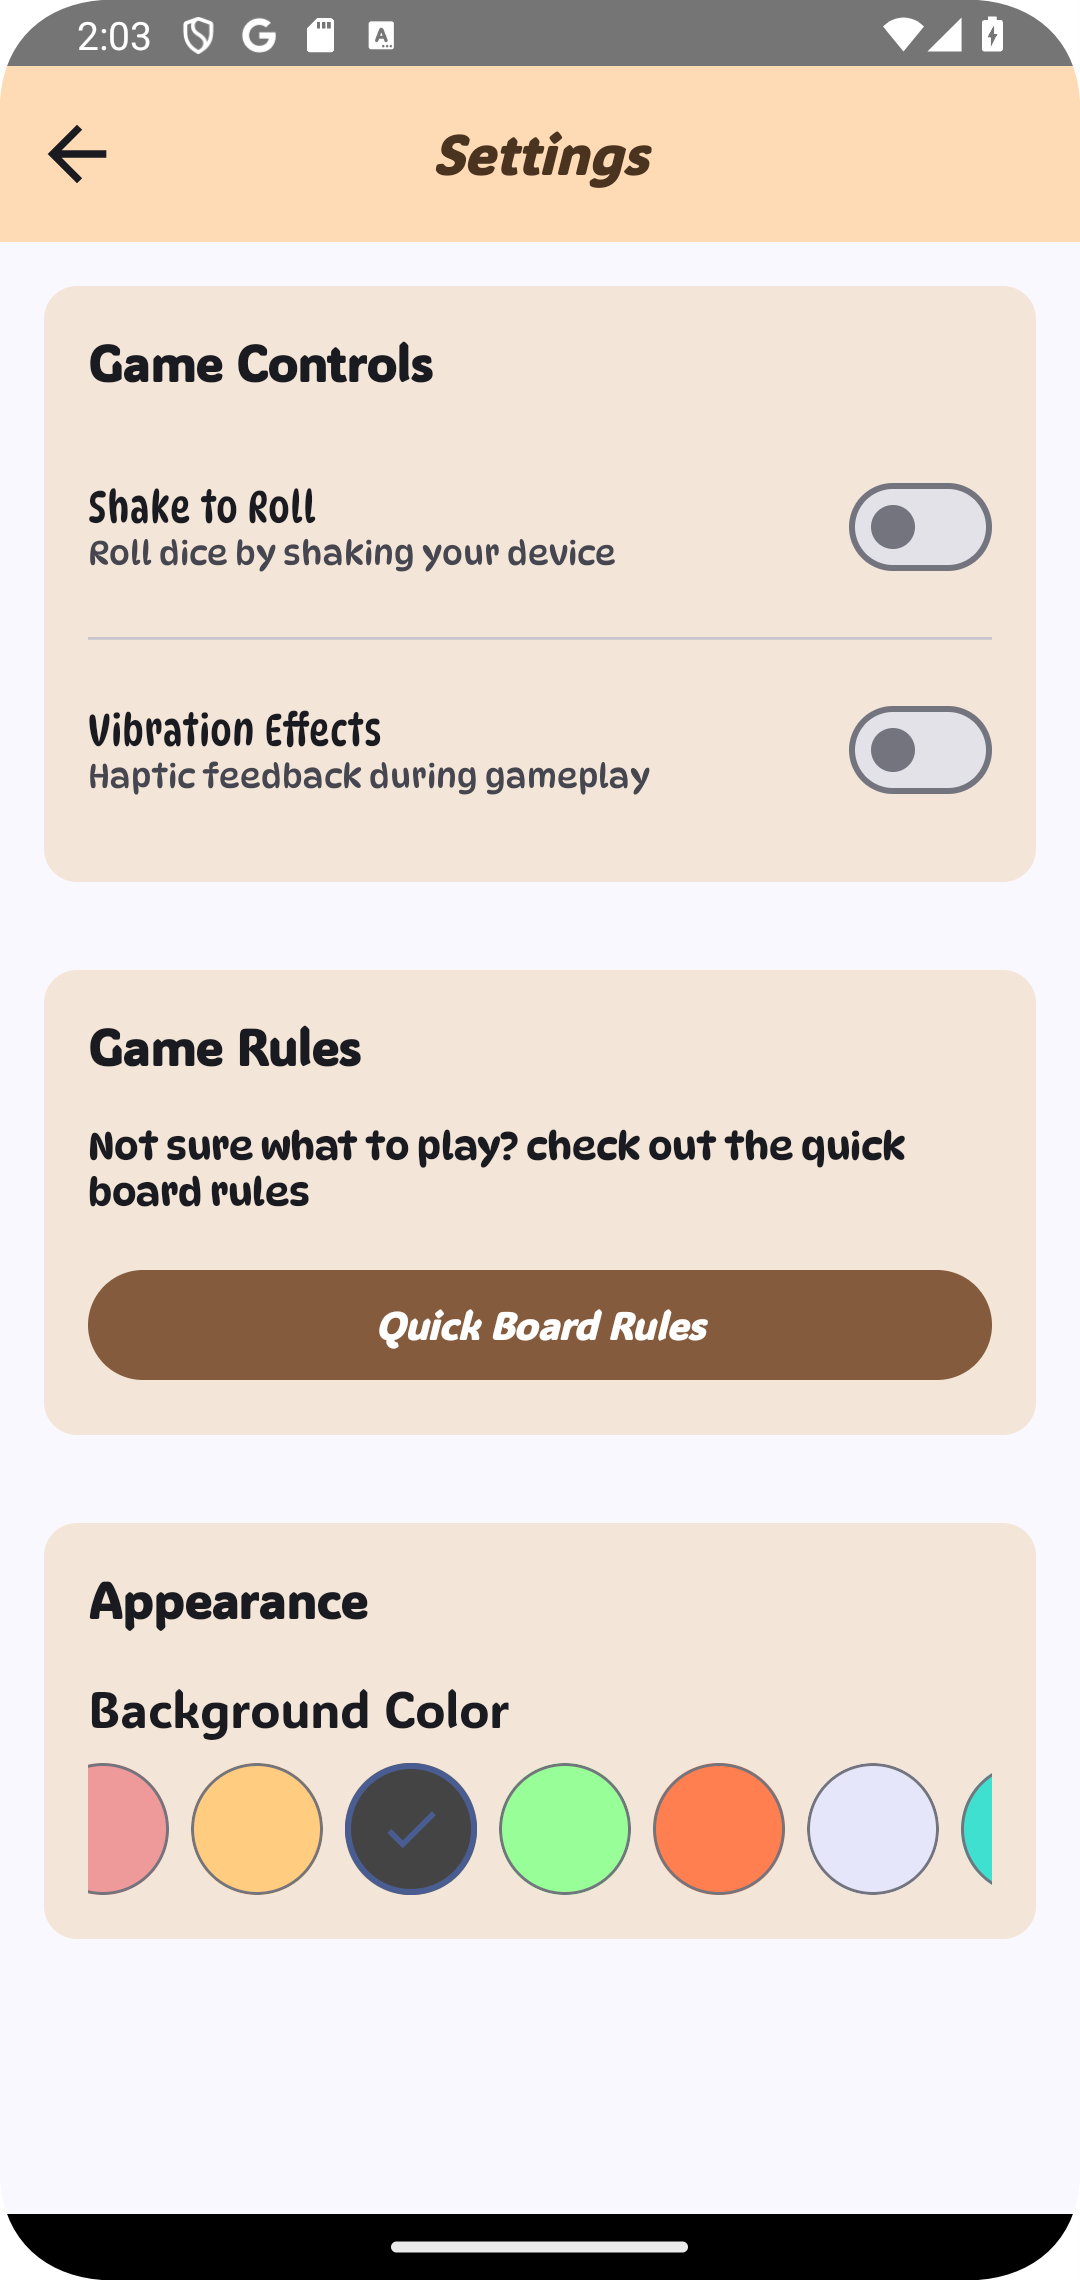
\includegraphics[width=\textwidth]{img/settings screen.png}
        \caption{Settings Screen}
        \label{fig:settings_screen}
    \end{subfigure}
    \caption{Instructions and Settings.}
\end{figure}

\subsection{Statistics}

The statistics screen offers users comprehensive insights into their gameplay performance. It displays a variety of data, including win records, average scores, and other pertinent metrics. The figure~\ref{fig:statistics_screen} illustrates the statistics screen, where users can view their achievements, such as "High Roller," "Lightning Fast," and "Greed Guru." Additionally, users can assess their risk-taking tendencies, current winning streaks, comebacks, and close games. The screen also features time analytics, allowing users to track their fastest games, total playtime, and time spent on individual games, providing a detailed overview of their gaming habits.
\begin{figure}[h]
    \centering
    \begin{subfigure}[b]{0.27\textwidth}
        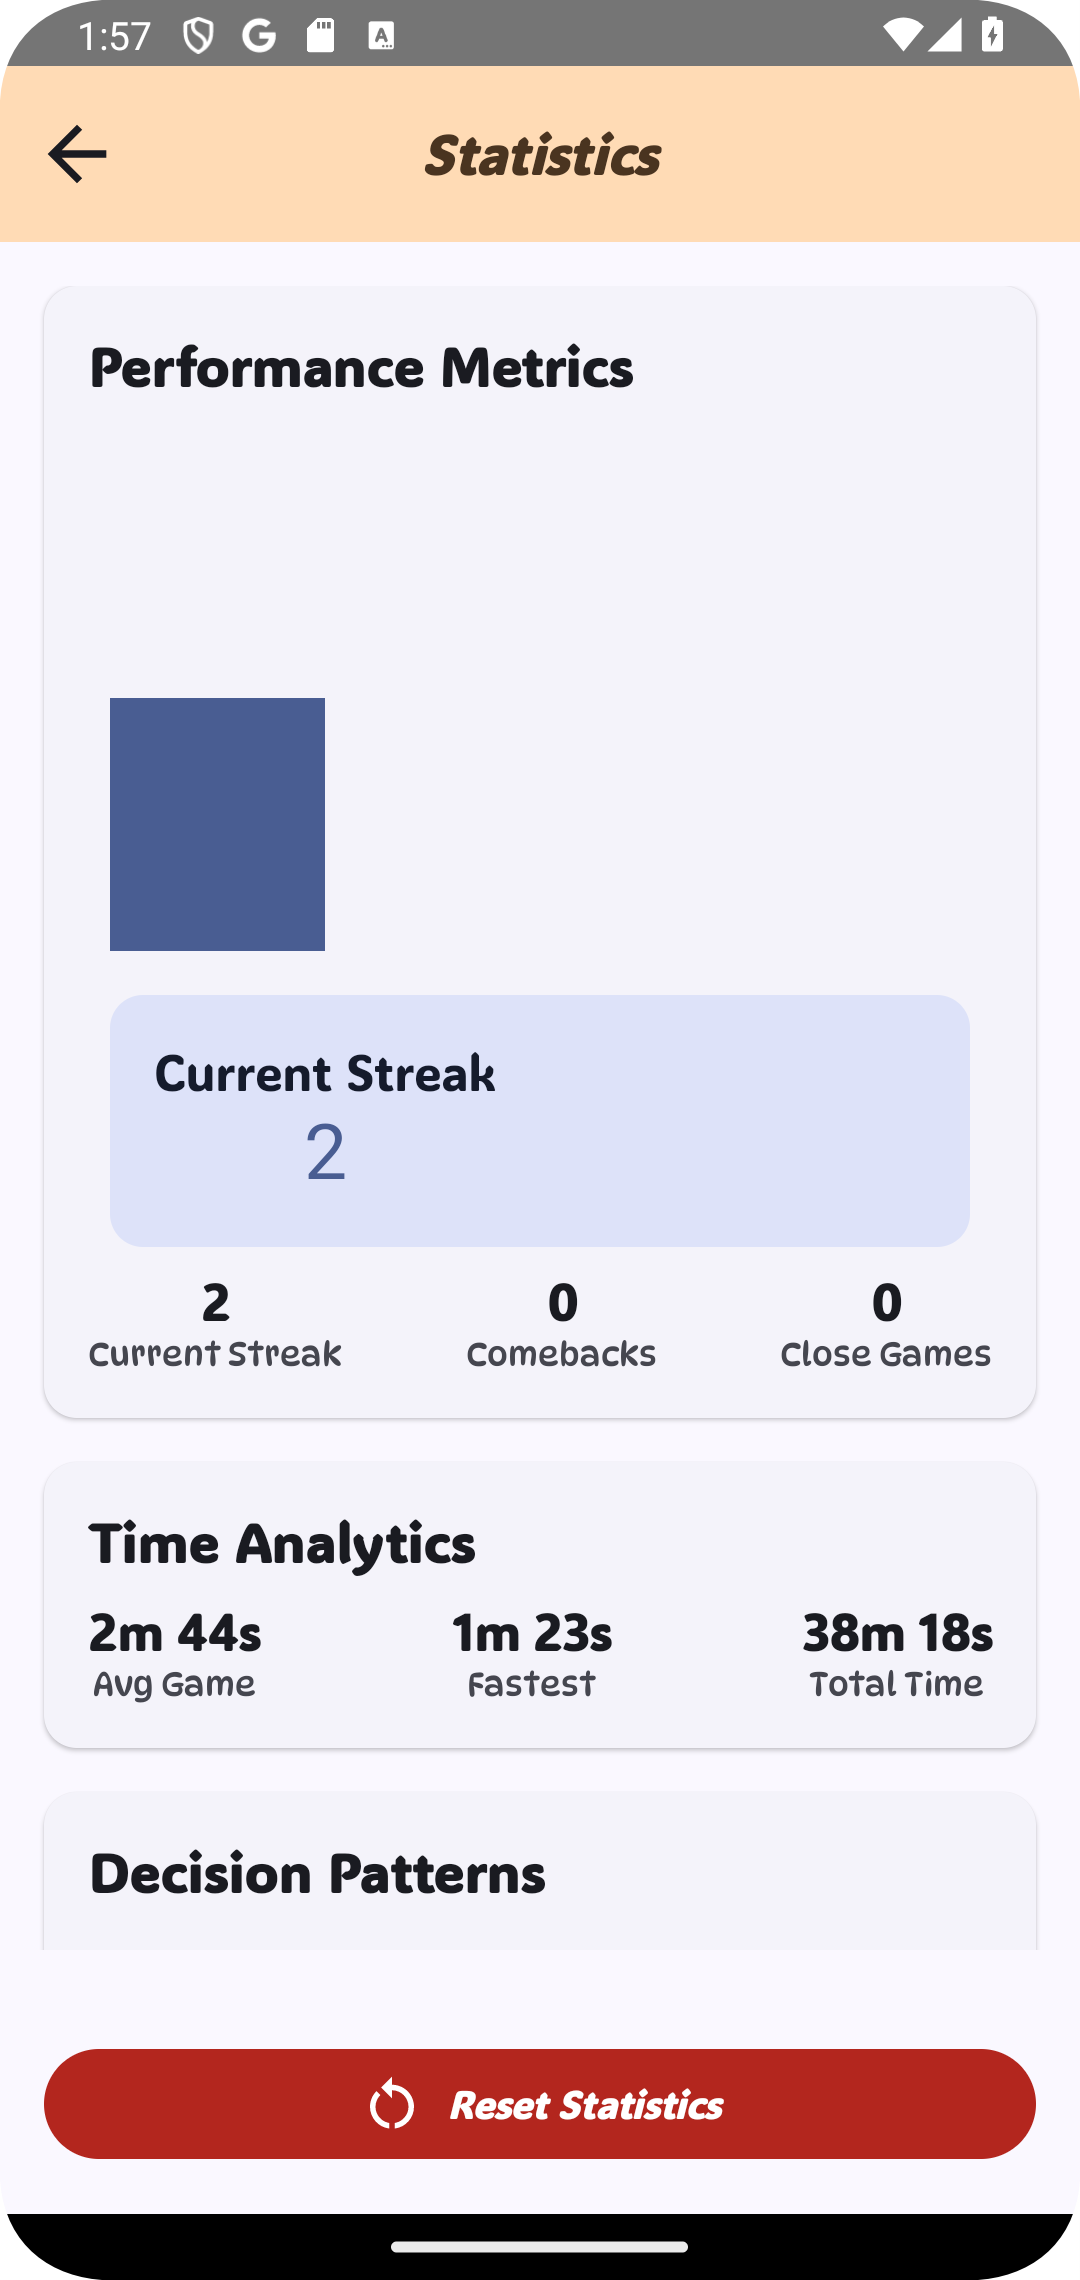
\includegraphics[width=\textwidth]{img/statistics screen.png}
        \caption{Performance Metrics}
    \end{subfigure}
    \hfill
    \begin{subfigure}[b]{0.27\textwidth}
        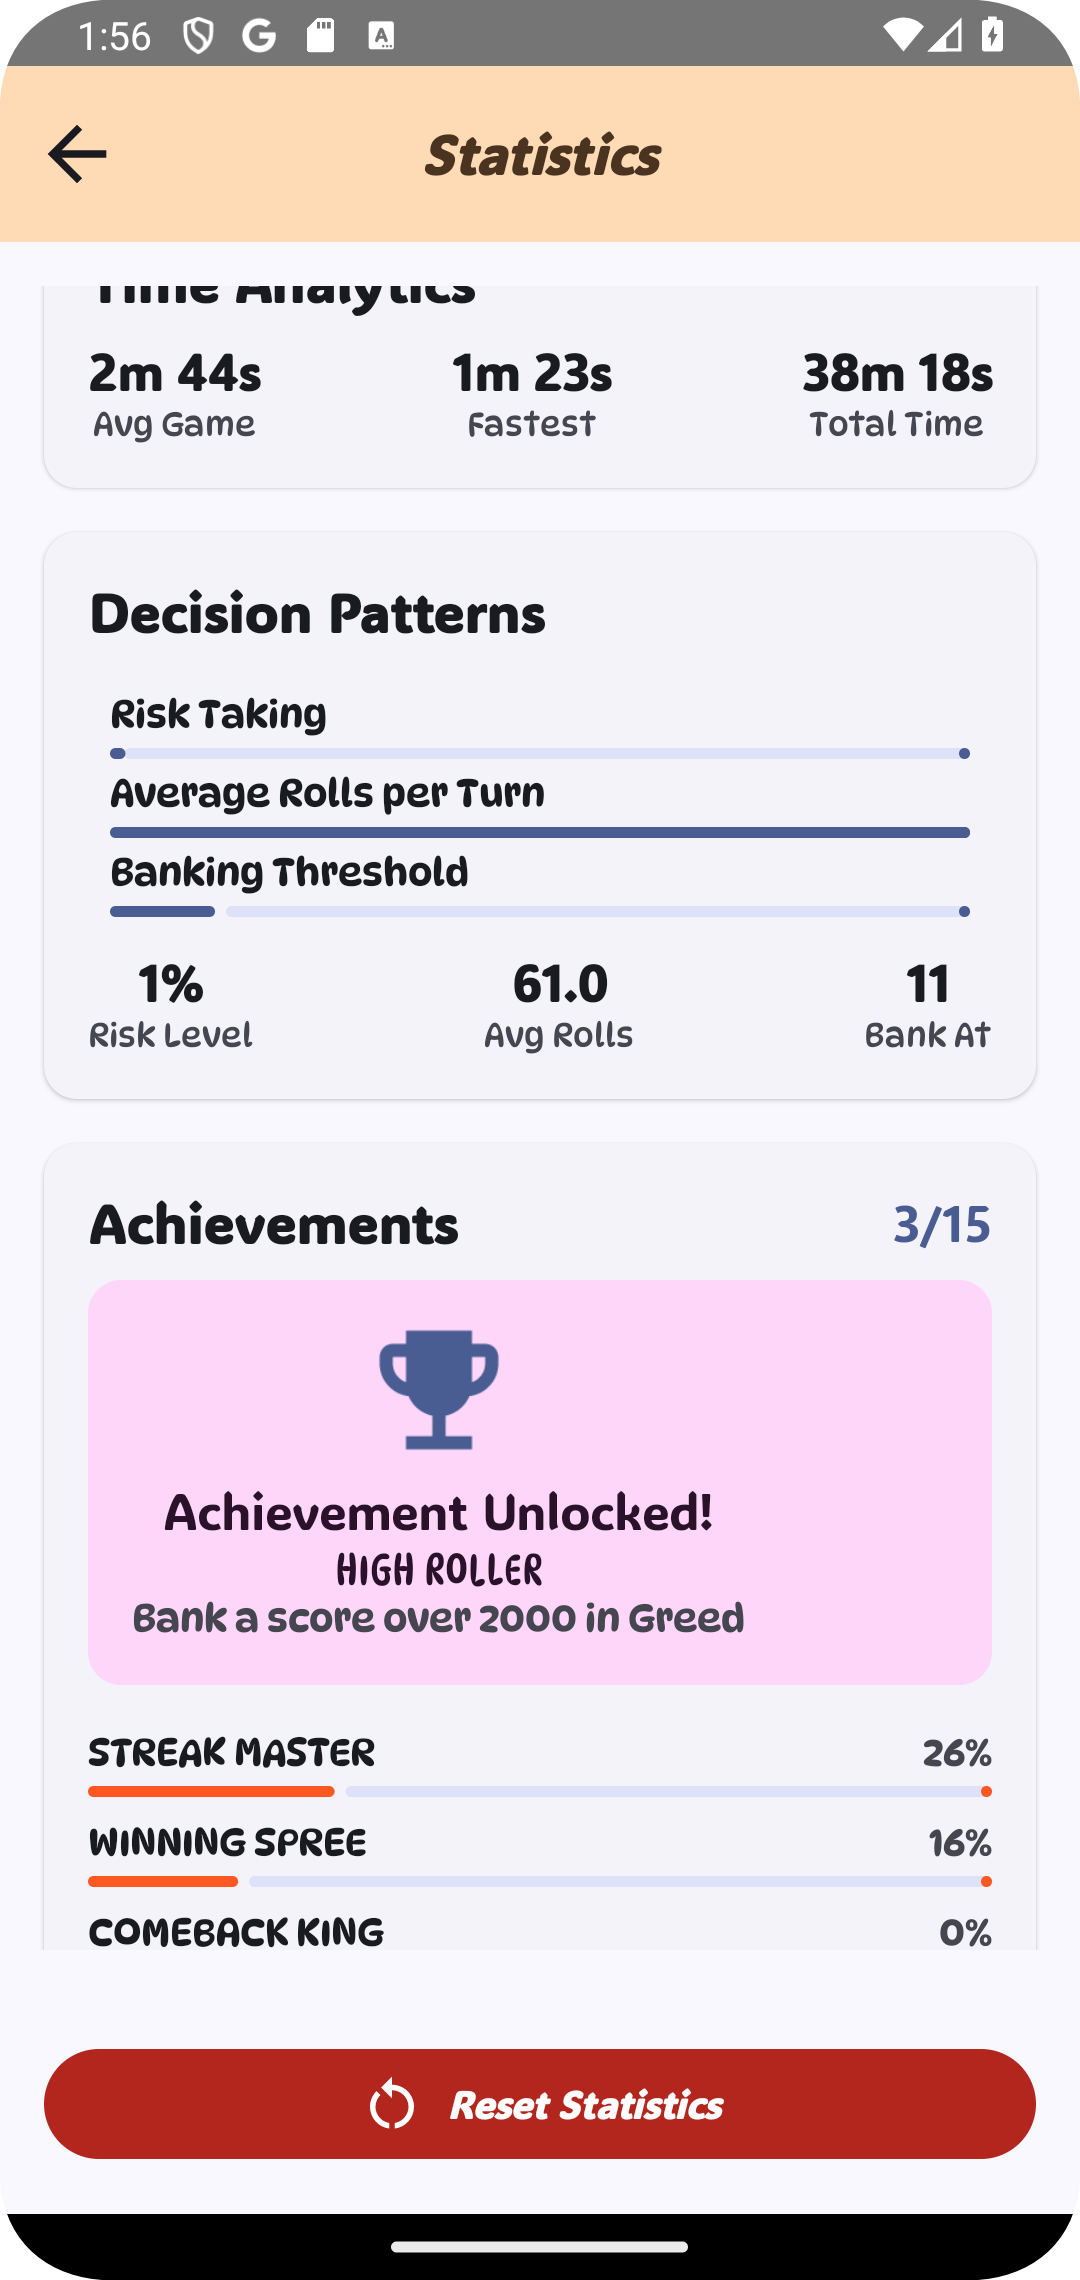
\includegraphics[width=\textwidth]{img/statistics screen3.png}
        \caption{Decision Patterns}
    \end{subfigure}
    \hfill
    \begin{subfigure}[b]{0.27\textwidth}
        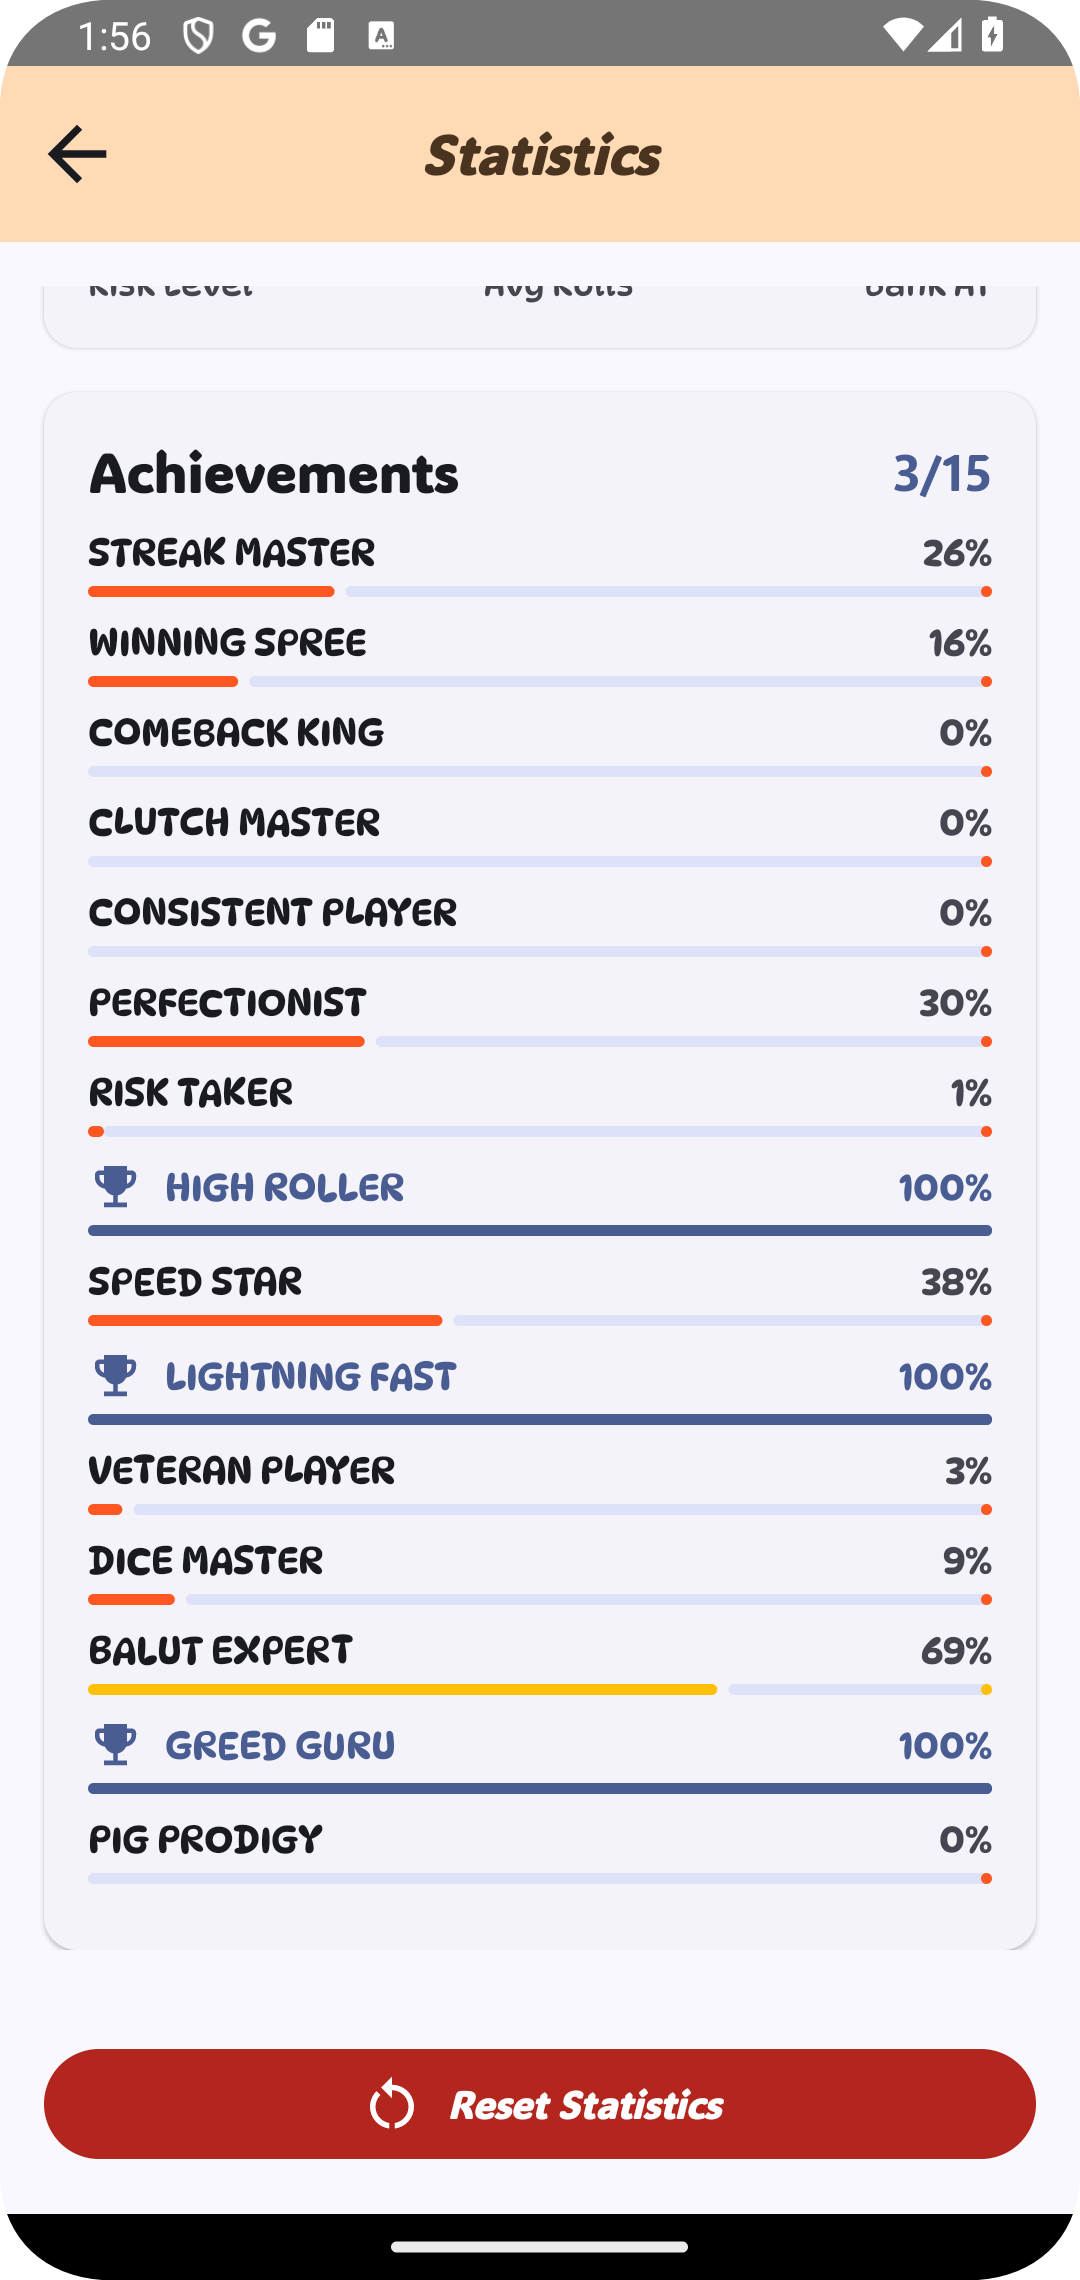
\includegraphics[width=\textwidth]{img/statistics screen2.png}
        \caption{Unlocking Achievements}
    \end{subfigure}
    \caption{Statistics Screen}
    \label{fig:statistics_screen}
\end{figure}

\section{System Administration}

The administration of the application involves several key tasks to ensure its reliability, performance, and security. These responsibilities are primarily carried out by the developers of the application, and can range from day to day maintenance to handling the occasional unforeseen issues.

\subsection{Application Maintenance}

Regular maintenance of the application is essential to ensure it remains functional and up to date. This involves several tasks, including:

\begin{itemize}
    \item \textbf{Release Management:} New releases of the application are periodically deployed via GitHub as APK releases, which often require careful planning and testing to ensure compatibility and maintain a consistent user experience. This includes creating new release branches, building the APK, and updating the app with new changes, new features, or bug fixes.
    \item \textbf{Monitoring and Troubleshooting:} Developers are also responsible for monitoring the performance of the application. This may involve checking for crashes, logging error reports, identifying bugs or unexpected behavior, and making changes to solve the issues.
\end{itemize}

\subsection{Data Management}

Careful management of the application data is critical to ensure its proper functioning.  The developers are responsible for \textit{DataStore Management}, which involves taking periodic backups of application settings and user preferences stored with Android DataStore. The data is also cleaned periodically to ensure that the device is not using unnecessary storage. This is essential to maintain consistency and avoid potential data corruption or data loss.

\section{Security Issues}
\subsection{Introduction}
This section provides a detailed view on the various security issues that the application is vulnerable to, based on potential threats and exploitable areas in the application.

\subsection{Data Handling}

Application data, including DataStore backups, might be accessed through Android's backup services if a user's Google account is compromised. Specifically, an attacker might be able to get access to the application if a user's Google account has been \textit{phished}, or if there has been a \textit{data breach}, or if the account has been compromised in some other way.

A compromised Google account could allow an attacker to access backups stored in Google Drive, potentially revealing all user information stored in the application.

The application uses Android's KeyStore to encrypt the backup data, however, this is not a full solution and does not prevent unauthorized access \cite{bib:android_data_backup}.

\subsection{Communication and API}
Even when using HTTPS, attackers can intercept data during transmission to the RoboFlow API. An attacker on the same network as the user can set up a malicious server and redirect all API requests to it, thereby gaining access to the API traffic. The application enforces HTTPS for all API requests, but it does not use certificate pinning, which means it is vulnerable to \textit{man in the middle} attacks. This is something that should be considered for future versions of the application. A sophisticated attacker could potentially bypass the HTTPS certificate and redirect the traffic through a malicious server. \cite{bib:owasp_top_ten}

Even with rate-limiting, attackers can bypass limitations and create a denial of service attack, potentially making the app or the external API unusable. A bot could flood the application with API requests. The application uses rate-limiting using a `CoroutineScope` and a `MutableStateFlow` to limit how many times an API is called in a given time, this does reduce the risk of the application crashing, but it is not foolproof. It also has input validation to prevent \textit{API abuse}, but these are not foolproof solutions and might be bypassed by sophisticated attackers.

\subsection{Code Security}

Even when using code obfuscation, attackers can still reverse engineer the code to steal private information and private API keys, or understand the game logic. Code Obfuscation is the process of making the code more difficult to read and understand, by changing the variable names, and classes to make them unreadable.

An attacker can decompile the application to find API keys that are used to contact external resources, or understand the game logic to make a bot to cheat at the game.

The application uses code obfuscation through R8's obfuscation process, to hide the code logic, which is not a full solution, and can be bypassed by sophisticated attackers \cite{bib:android_obfuscation}.

\section{Security Considerations}

The application implements several security measures to protect user data and ensure system integrity. These measures are based on Android security best practices and are designed to comply with relevant data protection requirements.

\subsection{Data Protection}

\begin{itemize}
    \item \textbf{Encrypted Local Storage:} User settings and preferences, saved using DataStore, are stored using Android's EncryptedSharedPreferences, which provides encryption at rest using Android's KeyStore.
    \item \textbf{Privacy-Preserving Image Processing:} Images captured by the user are only processed within the app's scope and are not stored or transmitted outside of the device unless explicitly requested by the user through a sharing action. No personally identifiable information is extracted and saved from the image.
\end{itemize}

\subsection{System Security}

\begin{itemize}
    \item \textbf{Runtime Permission Management:} The application requests only the necessary permissions at runtime (e.g., camera access) and respects the user's choice to grant or deny them. The application uses Android's Permission API to handle the permissions.
    \item \textbf{Secure Communication Channels:} The communication with the RoboFlow API for image recognition is done over HTTPS, which uses TLS/SSL encryption to ensure confidentiality and integrity of the API requests.
     \item \textbf{Data Access Controls:} Only the application can access the DataStore data, and only the specific components of the application that require it can access its underlying data. This reduces the risk of potential data exposure to malicious application or rogue modules of this application.
\end{itemize}

\subsection{Future Enhancements}

The following security enhancements are considered for future development:

\begin{itemize}
    \item \textbf{User Authentication and Authorization:}  Implementing a secure user authentication mechanism (e.g., using Firebase Authentication) and role-based authorization to enhance data protection and prevent unauthorized access to sensitive features, such as statistics or training data.
    \item \textbf{Improved API Security:} Implementing API rate-limiting to prevent abuse and implementing stricter input validation for the RoboFlow API.
     \item \textbf{Regular Security Audits:} Implementing regular penetration testing to evaluate the security and performance of the system.
\end{itemize}

\section{Working scenarios}

In addition to the scenarios described in the user manual \ref{sec:user_manual}, this section provides a few practical examples of application usage.

\begin{figure}[h]
    \centering
    \begin{subfigure}[b]{0.27\textwidth}
        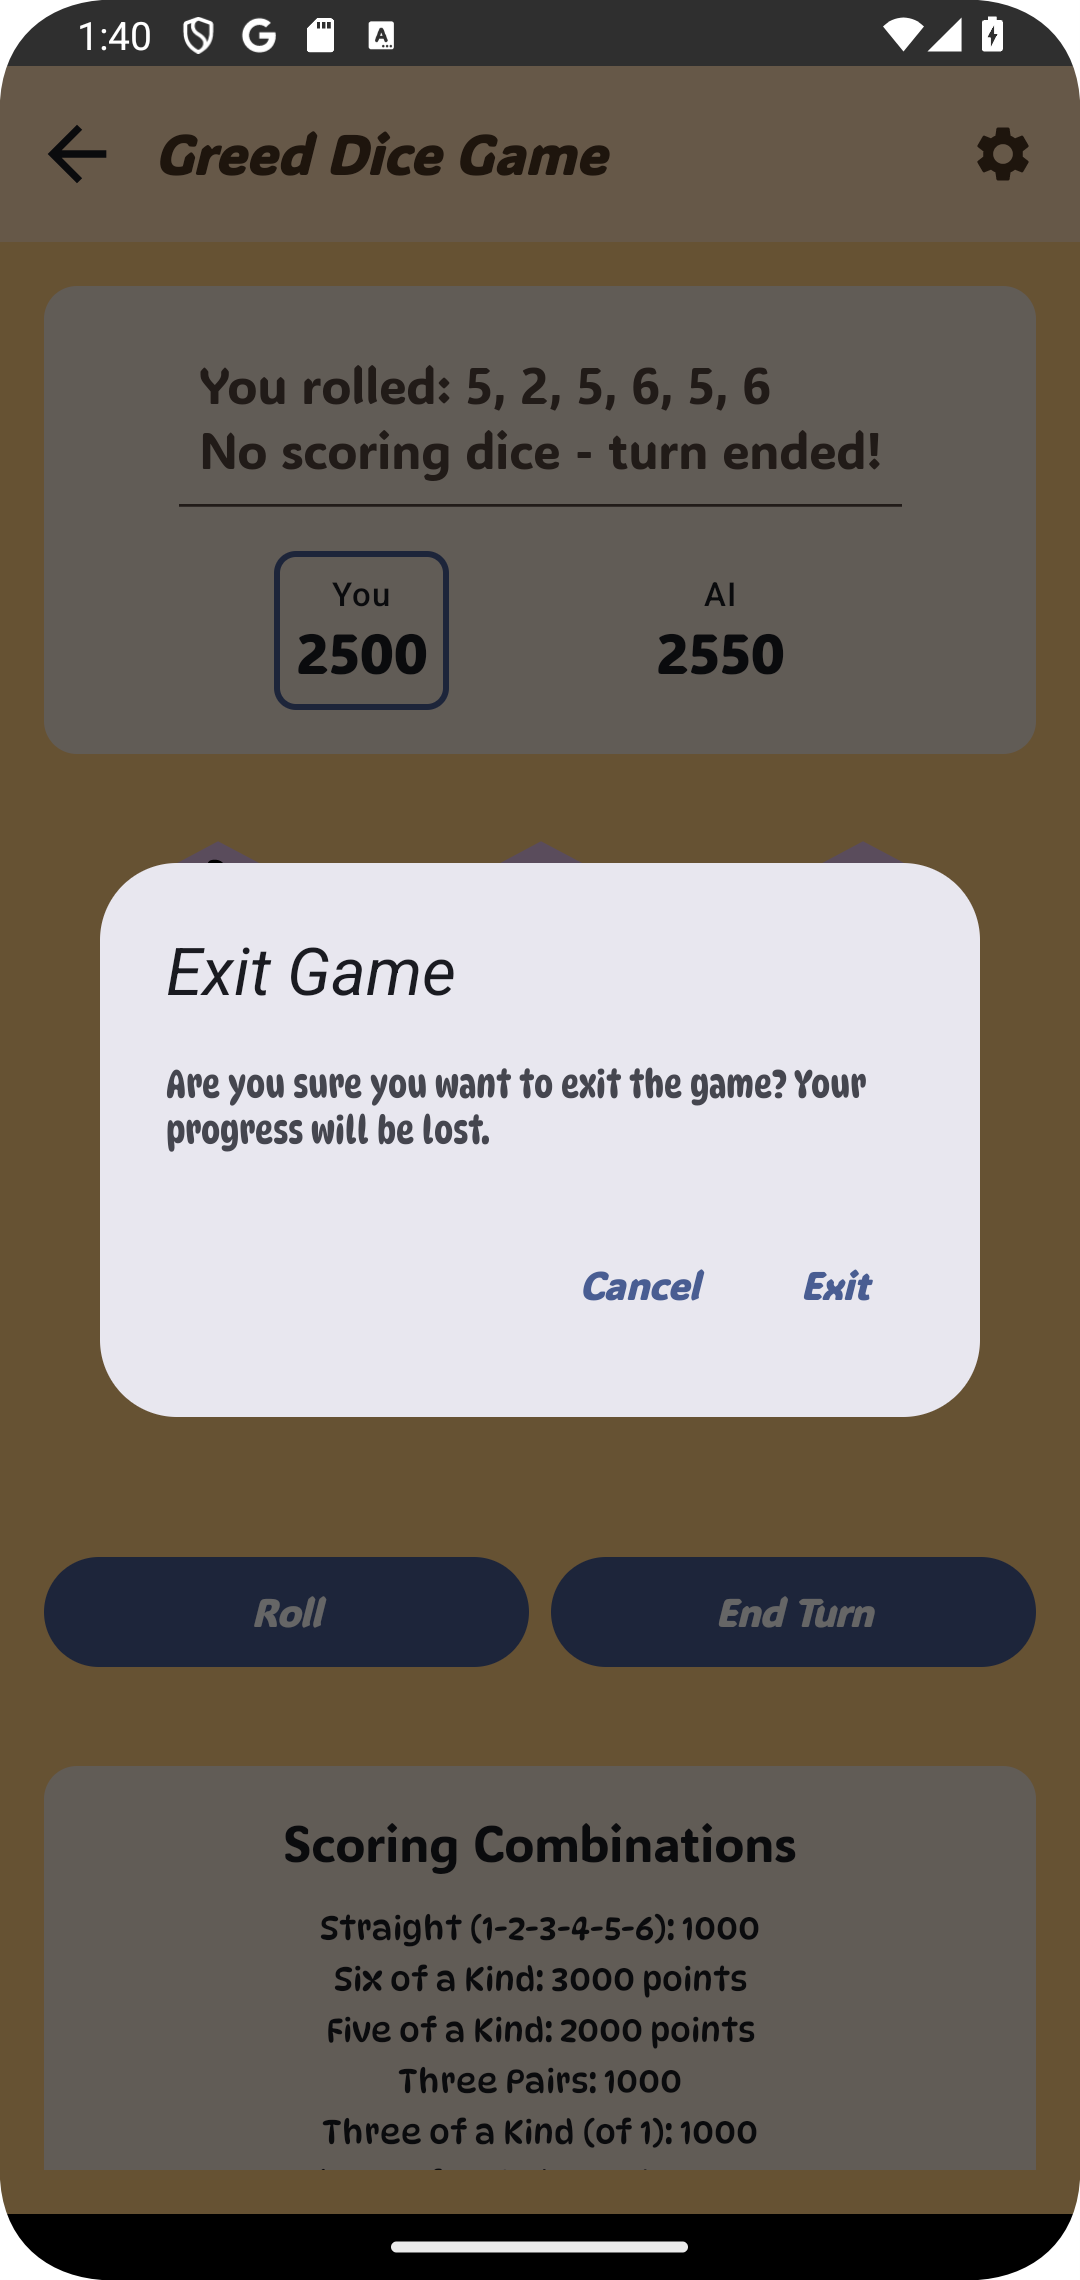
\includegraphics[width=\textwidth]{img/greed board2.png}
        \caption{Exiting a game of Greed}
    \end{subfigure}
    \hfill
    \begin{subfigure}[b]{0.27\textwidth}
        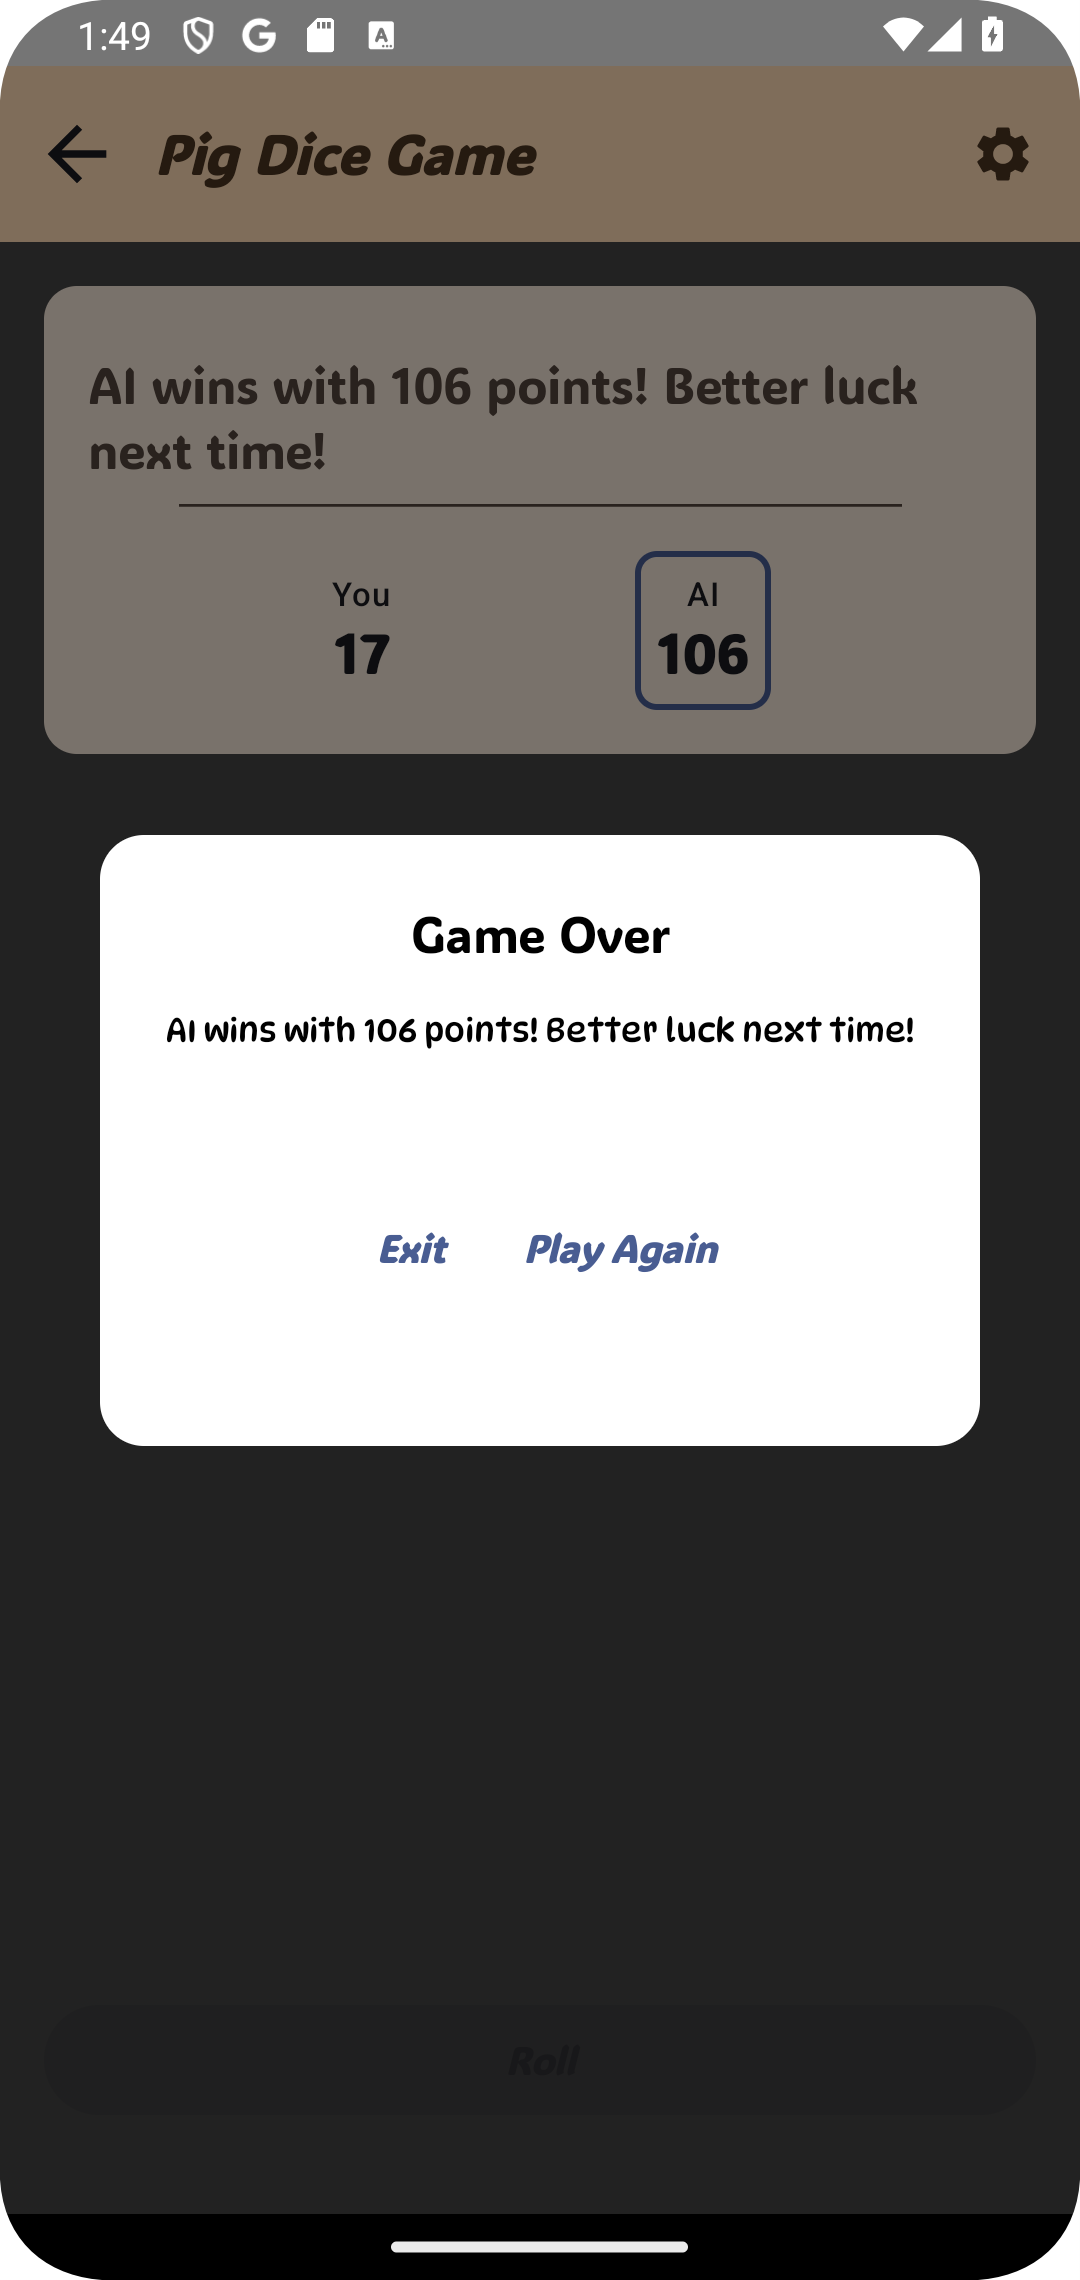
\includegraphics[width=\textwidth]{img/pig board2.png}
        \caption{Loosing a Game of Pig}
    \end{subfigure}
    \hfill
    \begin{subfigure}[b]{0.27\textwidth}
        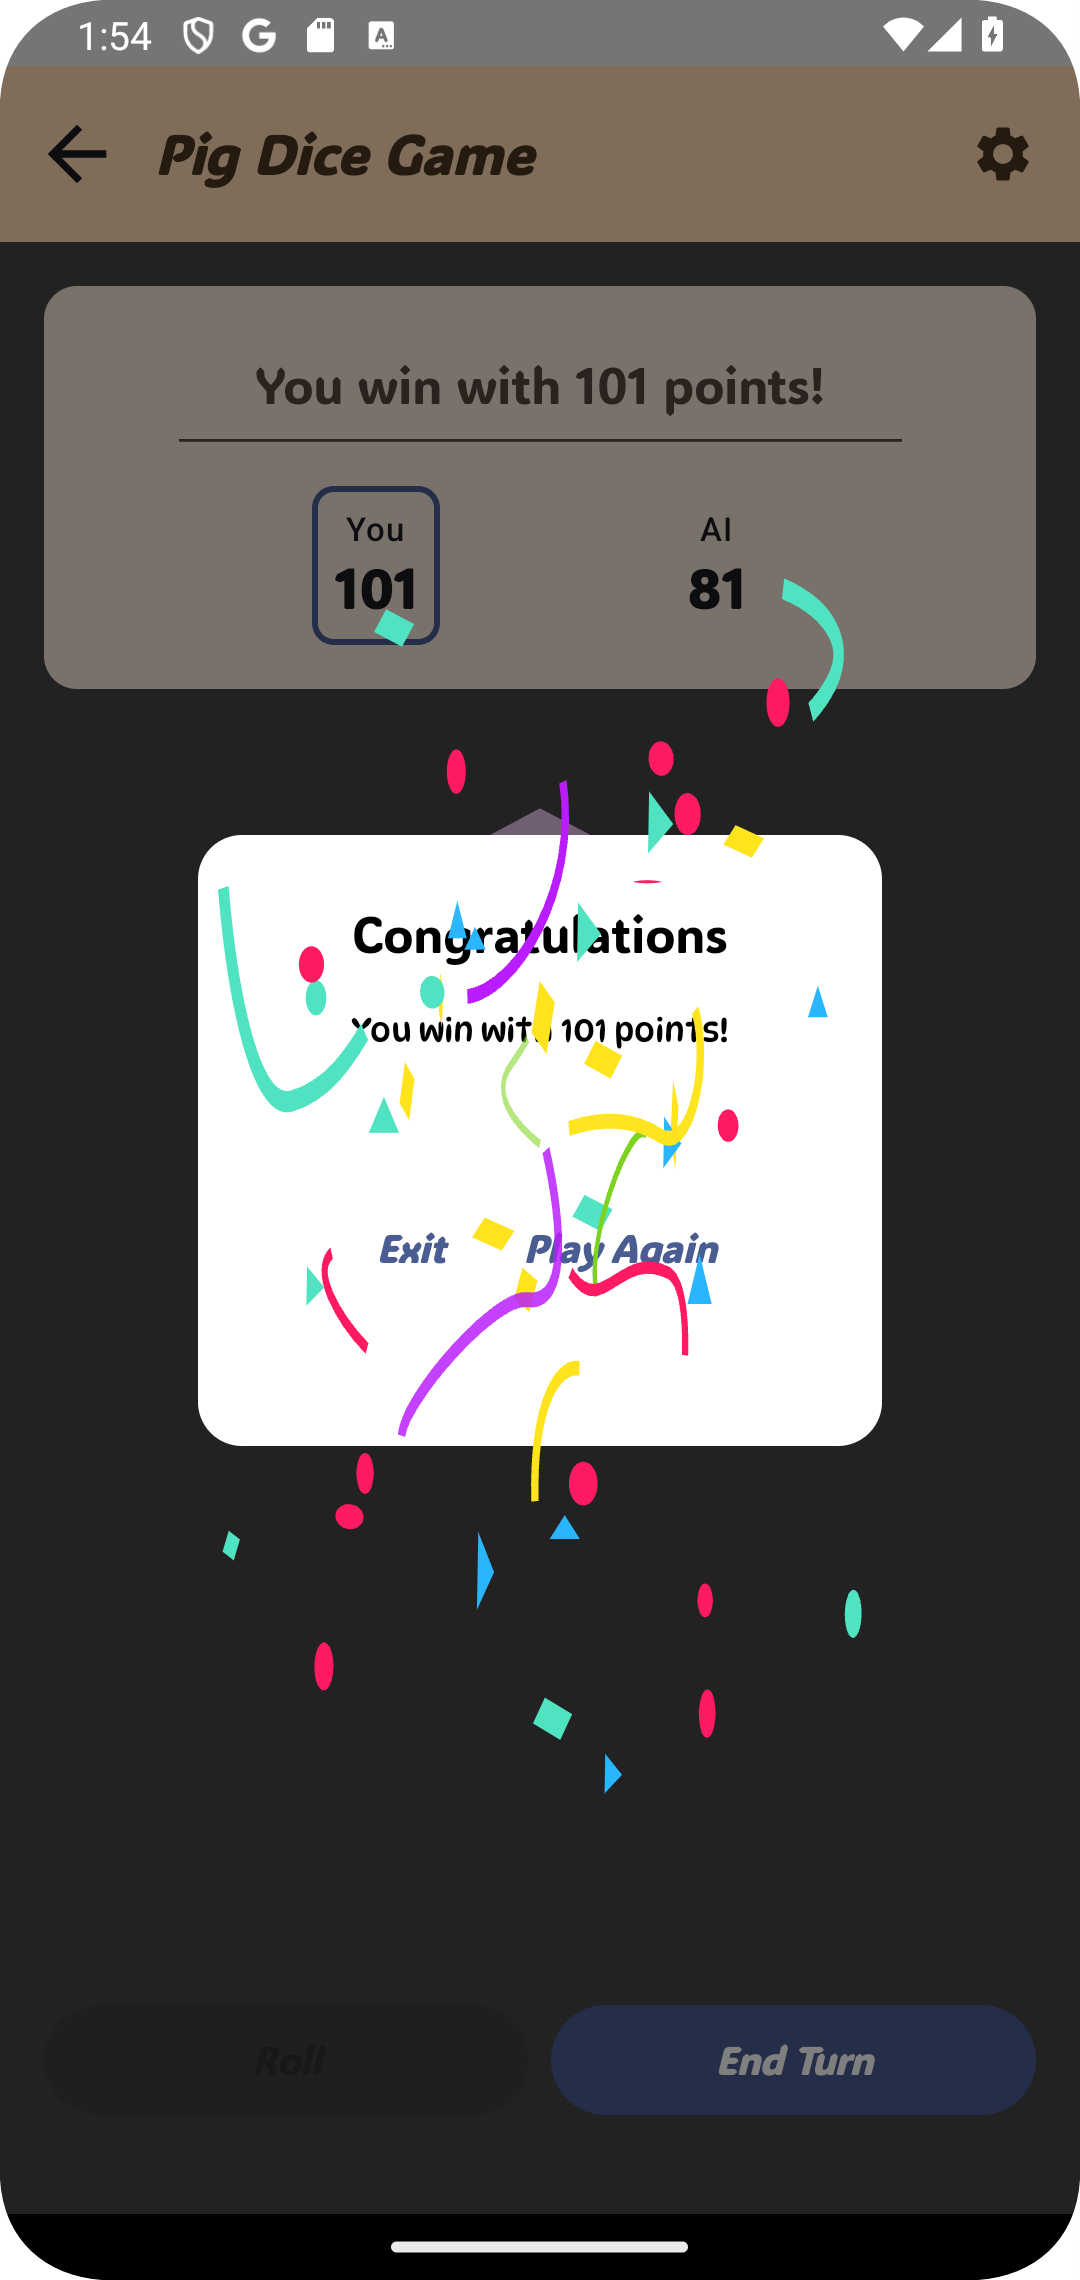
\includegraphics[width=\textwidth]{img/pig board3.png}
        \caption{Winning a Game of Pig}
    \end{subfigure}
    \caption{Board Features in the Application}
\end{figure}

\begin{figure}[ht!]
    \centering
    \begin{subfigure}[b]{0.27\textwidth}
        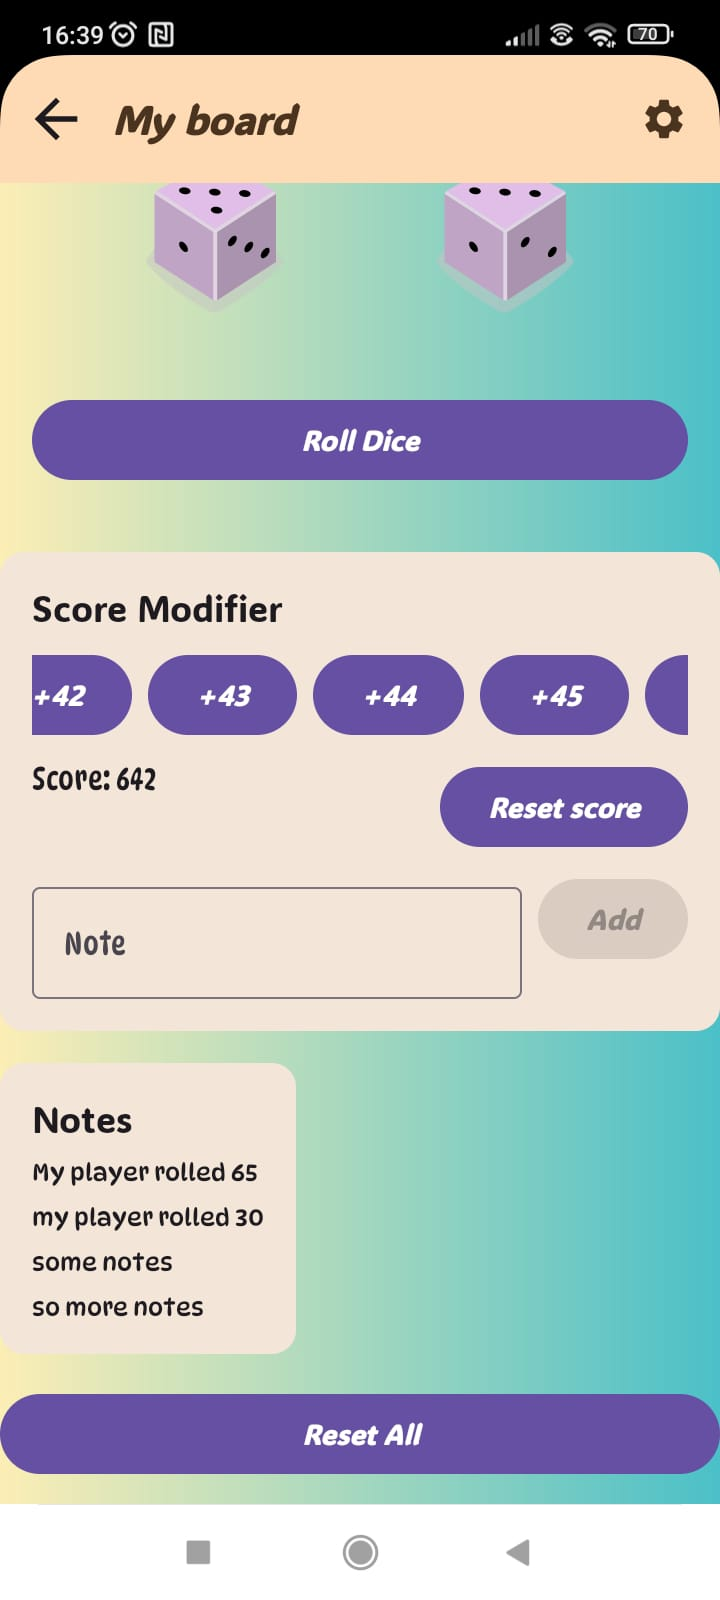
\includegraphics[width=\textwidth]{img/custom game.jpg}
        \caption{Custom Game Board}
    \end{subfigure}
    \hfill
    \begin{subfigure}[b]{0.27\textwidth}
        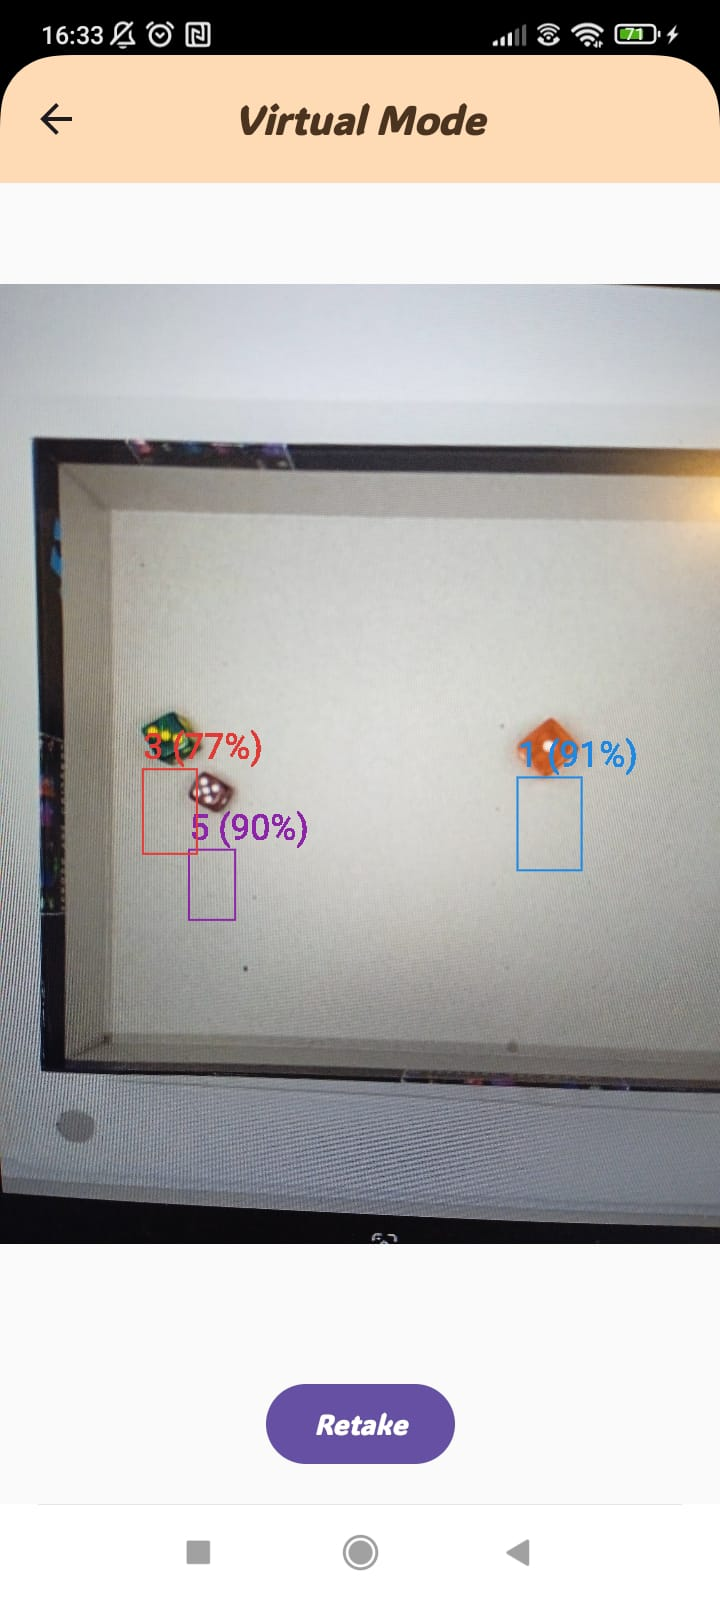
\includegraphics[width=\textwidth]{img/virtual screen2.jpg}
        \caption{Image Recognition Example}
    \end{subfigure}
    \hfill
    \begin{subfigure}[b]{0.27\textwidth}
        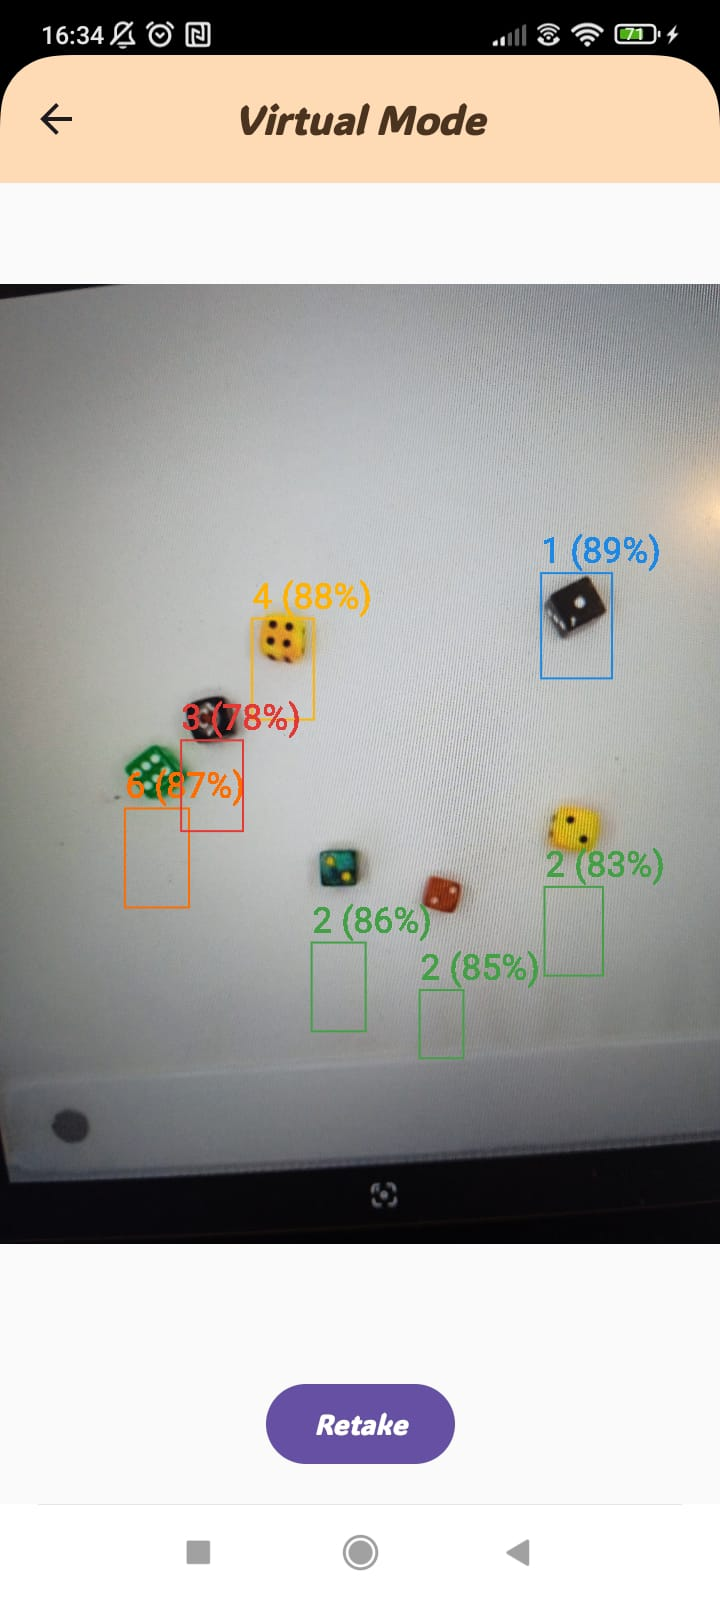
\includegraphics[width=\textwidth]{img/virtual screen.jpg}
        \caption{Image Recognition Example 2}
    \end{subfigure}
    \caption{Additional Features and Interactions}
\end{figure}

\chapter{Internal Specification}
\label{chap:internal-specifications}

This chapter provides a detailed overview of the application's internal workings. It covers the system's concept, architecture, data structures, components, algorithms, design patterns, and relevant UML diagrams.

\section{System Architecture}

The project's architecture follows the modern Model-View-ViewModel (MVVM) pattern, adhering to Clean Architecture principles. This separation of concerns allows for better maintainability and testability of the code.

\begin{figure}[ht!]
    \centering
    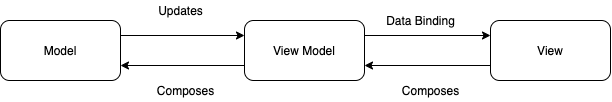
\includegraphics[width=0.7\textwidth]{img/mvvm_explanation.png}
    \caption{High Level MVVM Architecture.}
    \label{fig:mvvm_explanation}
\end{figure}

As shown in Figure~\ref{fig:mvvm_explanation}, the application is structured into several layers~\cite{bib:mvvm}:

\begin{itemize}
    \item \textbf{Application Layer}: Contains the main application logic and navigation.
    \item \textbf{UI Layer}: Responsible for the user interface components, including screens and themes. This layer corresponds to the "View" component of the MVVM pattern.
    \item \textbf{ViewModel Layer}: Manages the data and business logic, providing a bridge between the UI and the Model. This layer corresponds to the "ViewModel" component of the MVVM pattern.
    \item \textbf{Manager Layer}: Handles specific game logic and state management. This layer sits below the view model, and contains the logic for manipulating the models.
    \item \textbf{Repository Layer}: Manages data access and interactions with external sources. This layer is the gatekeeper for the model layer, accessing and manipulating the models before passing it to the application layer.
    \item \textbf{Model Layer}: Represents the data and domain logic of the application. This layer contains the data entities and business rules. This layer corresponds to the "Model" component of the MVVM pattern.
\end{itemize}


\section{Methodology of Design and Implementation}

The design and implementation of the dice game application follow an iterative and incremental development methodology. This approach involves:
\begin{enumerate}
    \item \textbf{Requirement}: Identifying and documenting functional and non-functional requirements.
    \item \textbf{Design}: Creating architectural and component designs, including UML diagrams to visualize system interactions.
    \item \textbf{Implementation}: Developing the application in iterative cycles, focusing on one feature or component at a time.
    \item \textbf{Testing}: Conducting unit, integration, and user acceptance testing to ensure the system meets requirements using JUnit.
    \item \textbf{Documentation}: Documentation of the implemented features and future development possibilities.
\end{enumerate}

\begin{figure}[ht!]
    \centering
    \begin{subfigure}[b]{0.48\textwidth}
        \centering
        
\includegraphics[scale=0.45]{img/play.png}
        \caption{Design Page 1}
        \label{fig:figma_design1}
    \end{subfigure}
    \hspace{0.02\textwidth}
    \begin{subfigure}[b]{0.48\textwidth}
        \centering
        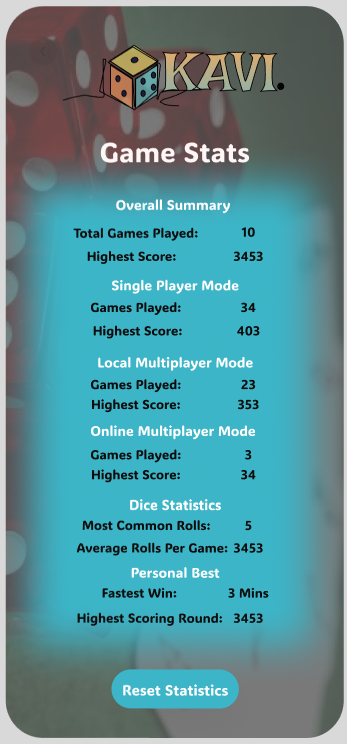
\includegraphics[scale=0.45]{img/stats.png}
        \caption{Design page 2}
        \label{fig:figma_design2}
    \end{subfigure}
    \caption{Initial UI designs and prototypes created in Figma}
    \label{fig:figma_designs}
\end{figure}

\subsection{Design Process}
The application's design process began with creating detailed wireframes and prototypes in Figma. The designs underwent several iterations based on user feedback and technical constraints, evolving into the final implementation. Figure~\ref{fig:figma_designs} shows some of the initial design concepts and their evolution~\cite{bib:kavifigma}.

Various existing solutions and design tools inspired the design of the application, one of which stood out was the board screen design was inspired by a dice application project by Shreyansh Saurabh~\cite{bib:binaryshrey}. This repository provided a minimalistic and intuitive approach to dice roll applications, which influenced the layout and functionality of the board screen in this project.

\subsection{Model Training}

The dice detection model was developed using Roboflow's platform, which streamlined the entire process from dataset creation to deployment. The training dataset, shown in Figure~\ref{fig:roboflow_dataset}, consisted of carefully annotated dice images across various conditions, ensuring robust detection performance in real-world scenarios.

\begin{figure}[ht!]
    \centering
    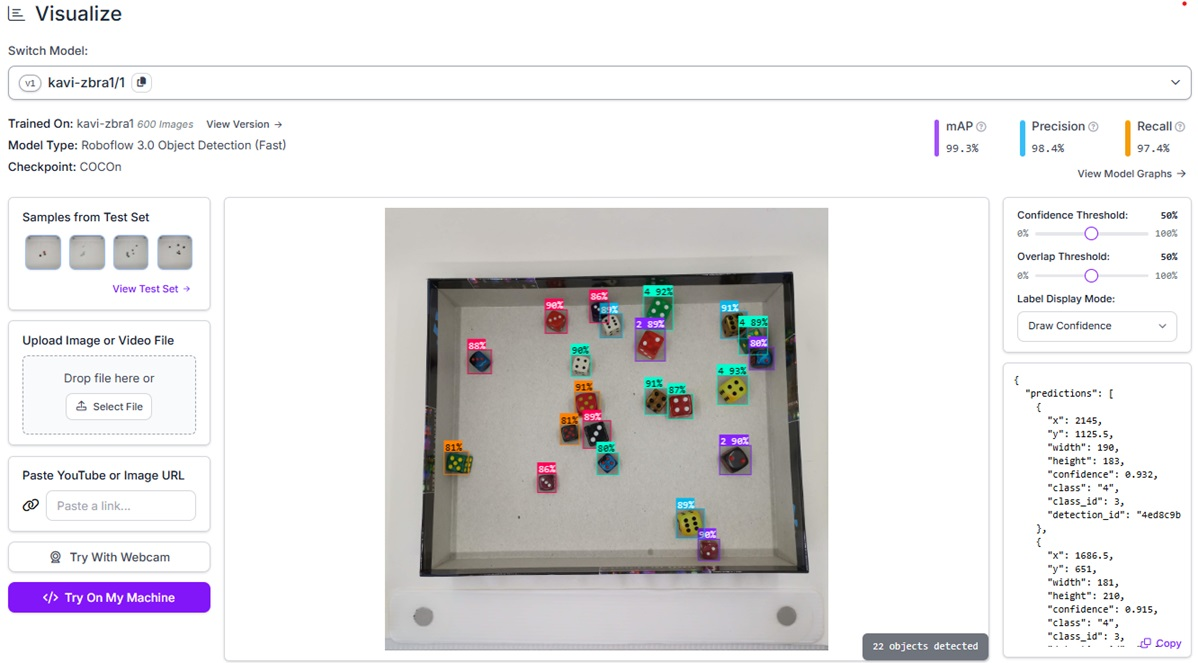
\includegraphics[width=\textwidth]{img/roboflow_dataset.jpg}
    \caption{Roboflow dataset management interface showing dice image annotations}
    \label{fig:roboflow_dataset}
\end{figure}

Roboflow facilitated data augmentation and preprocessing, which enhanced the dataset's diversity. The model training and optimization phases were crucial for achieving high accuracy, while the deployment and API integration ensured seamless real-time inference capabilities.

\subsection{Project Timeline}

The project was implemented following a structured timeline as shown in Figure~\ref{fig:gantt}. The development process was organized into major phases, including planning, design, core development, AI integration, and testing, with regular milestones to track progress.

\begin{figure}[ht!]
    \centering
    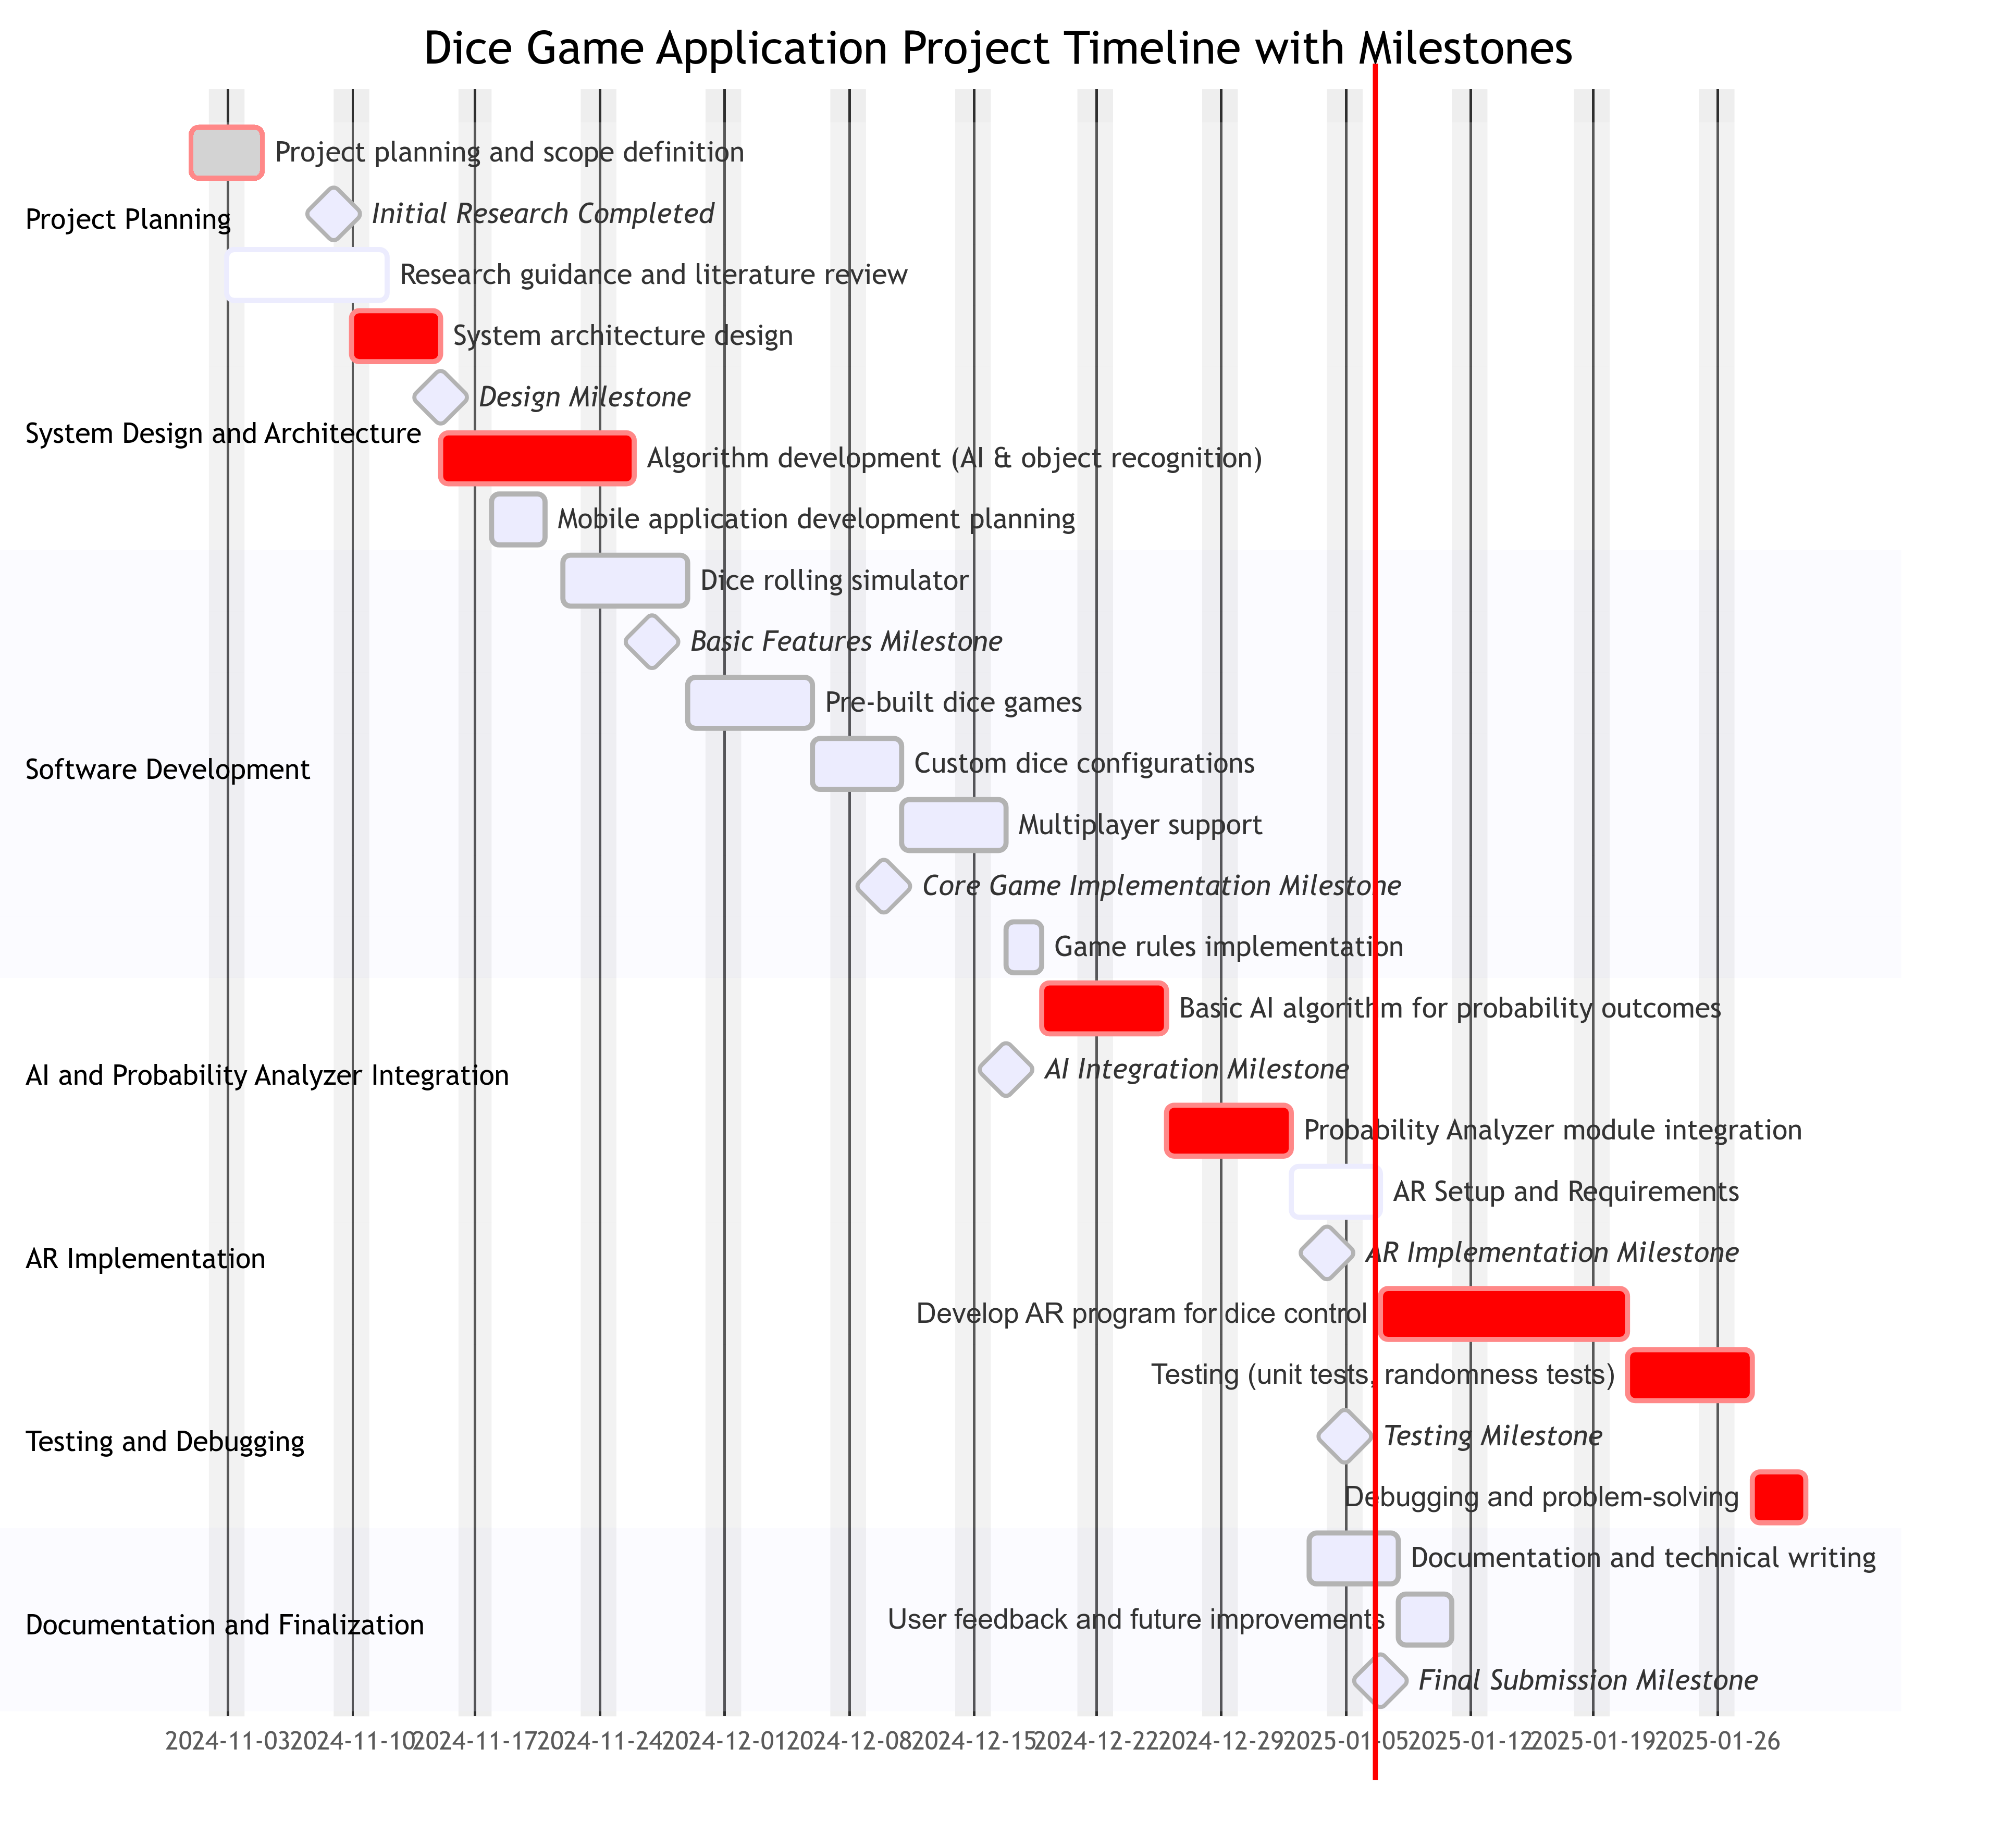
\includegraphics[width=\textwidth]{img/gantt_chart.png}
    \caption{Project Gantt chart showing development phases and milestones}
    \label{fig:gantt}
\end{figure}

This structured approach allowed for continuous improvement and adaptation to changing requirements, ensuring a high-quality application. While some initially planned features like AR implementation were identified as future enhancements, the focus remained on delivering a robust core game experience with AI capabilities.

\section{Data Structures and Data Management}

The application utilizes a variety of data structures to effectively manage game state, user profiles, and game data. These structures are designed for efficiency and scalability, supporting the diverse features of the game. Data persistence is achieved using DataStore, a modern data storage solution, and dependency injection is managed using Dagger Hilt.

\subsection{Data Models}

The application's data is represented using models located in the `models` directory. These models encompass different aspects of the game, including game state, user data, and results from the image detection mechanisms.

\subsubsection{Game Models}

The core game models are:
\begin{itemize}
    \item \textbf{GameStatistics}: Tracks overall game performance metrics for each user across all games. These metrics include total games played, win rates, average scores, and other relevant data.
    \item \textbf{GameScoreState}: Holds the current score and state of the game during an individual game session, including the score for each player and the game's current turn.
     \item \textbf{DecisionPatterns}: Captures the different decision-making patterns of a player in each game, including when the player decides to hold dice, or when they decide to roll or bank scores. This is used to calculate statistics about how players are playing the game.
    \item \textbf{WinRate}: Calculates and stores the win rate of a player. This will be used in \textit{PlayerAnalysis}.
    \item \textbf{TimeMetrics}: Stores metrics about how long a player played the game, including the amount of time a player has spent playing each game, and the time spent per round. This is used in \textit{PlayerAnalysis}.
    \item \textbf{PlayerAnalysis}: Provides detailed analysis of a player's behavior and performance trends, combining data from various sources like `WinRate`, `TimeMetrics`, and `DecisionPatterns`. It tracks trends over time, identify strong and weak areas of a player, and provides an overall evaluation of a player's performance.
\end{itemize}

\subsubsection{Detection Models}

The detection models, located in the `detection` subdirectory of `models`, are:

\begin{itemize}
    \item \textbf{DiceDetectionResult}: Captures results from dice detection processes, including the number detected and the number on each die.
    \item \textbf{Detection}: Represents the state of the detection model.
    \item \textbf{DetectionRequest}: Represents the request to start the detection.
    \item \textbf{DetectionResponse}: Represents the response from the detection.
    \item \textbf{ImageInfo}: Holds the information of the image used for detection.
    \item \textbf{Prediction}: Represents a single prediction from the detection model.
\end{itemize}

\subsection{Data Management}

The application uses a modern and efficient approach to data management, leveraging DataStore for persistent storage and Dagger Hilt for dependency injection.

\subsubsection{Persistent Storage}

DataStore provides a robust, asynchronous solution for managing the application's persistent data. Unlike traditional databases, DataStore offers type safety and a reactive approach, ensuring smooth and efficient data handling for user preferences, game statistics, and other relevant application data. This approach helps the application to provide quick access to stored data and avoids some of the limitations of other persistent storage options.

\subsubsection{Dependency Injection}
Dagger Hilt simplifies the management of dependencies by providing a standardized way to inject components into the application. This improves code modularity, making the app easier to test, maintain, and scale. Dagger Hilt helps manage the dependencies between classes and is used to ensure all modules are configured correctly, and this creates a more efficient way to manage the dependencies of the application, while also making testing easier.

\section{Components, Modules, and Classes}

This section outlines the core components, modules, and classes that form the foundation of the application. It provides a summary of essential classes, detailing their roles and responsibilities.

\subsection{Application Classes}
The main classes of the application can be categorized into Main Application Classes, ViewModels, and Managers.
\subsubsection{Main Application Classes}
\begin{itemize}
    \item \textbf{KaviApplication}: The main class that extends Android's Application class, responsible for initializing the application, and important libraries like Timber for debugging.
    \item \textbf{MainActivity}: The main entry point for the application, sets up the primary UI, and manages navigation.
\end{itemize}

\subsubsection{ViewModels}
\begin{itemize}
    \item \textbf{AppViewModel}: Manages application-wide data and state, coordinating between different parts of the application.
    \item \textbf{GameViewModel}: Manages data and logic specific to each game, providing a bridge between the view and the data and state.
    \item \textbf{DetectionViewModel}: Manages the state and logic of the image detection process, and exposes this data to the UI layer.
\end{itemize}

\subsubsection{Managers}
\begin{itemize}
    \item \textbf{MyGameManager}: Handles the state management and the logic of the custom game board.
    \item \textbf{PigGameManager}: Manages the game state, rules, and scoring for the Pig game.
    \item \textbf{GreedGameManager}: Manages the game state, rules, and scoring for the Greed game.
    \item \textbf{BalutGameManager}: Manages the game state, rules, and scoring for the Balut game.
    \item \textbf{DiceManager}: Manages the various aspects of rolling the dice, and its state.
    \item \textbf{DataStoreManager}: Manages the saving and retrieval of data from the DataStore.
    \item \textbf{StatisticsManager}: Manages the collection and processing of game statistics.
    \item \textbf{SettingsManager}: Manages the saving and loading of the application's settings.
    \item \textbf{ShakeDetectorManager}: Manages the logic of the shake gesture.
\end{itemize}

\vspace{0.2cm}
A detailed Class diagram is included in the UML diagram provided in Section~\ref{sec:uml}.

\section{Algorithms and Implementations}

The application implements several sophisticated algorithms to provide an engaging and intelligent gaming experience. 

\subsection{Image Processing Pipeline}

The dice recognition system uses a sequence of image processing steps implemented in `RoboflowRepositoryImpl`, a class responsible for handling communication with the Roboflow API:
\subsubsection{Preprocessing}
    \begin{itemize}
        \item RGB conversion using `ensureRGBFormat()` to guarantee that the image is in the correct format for processing.
        \item Contrast enhancement through `enhanceContrast()` using histogram-based normalization to make the dice pips more clear.
        \item Aspect ratio scaling via `scaleWithAspectRatio()` to make sure that the images are of the correct size.
        \item Noise reduction with `reduceNoise()` to reduce the noise in the image.
    \end{itemize}
\subsubsection{Detection}
    \begin{itemize}
        \item API integration with Roboflow service using the `RoboflowClient`, which makes a call to the Roboflow API and gets the result.
        \item Confidence filtering (threshold: 40\%) which removes detections with less than 40\% confidence to avoid erroneous detections.
        \item Non-maximum suppression, performed by using a library for detection, which removes overlapping bounding boxes, by selecting the bounding boxes with the highest score and removing those that are overlapping.
    \end{itemize}

\subsection{AI Strategy System}

The AI decision-making system, which is responsible for determining the optimal moves for the AI, is implemented across multiple manager classes. The strategy is designed to consider the current game state and make intelligent decisions based on the game variant. Below are the key methods used by the AI to guide its decisions:
    
\begin{itemize}
\item  \textit{`shouldAIBank()`} is responsible for determining when the AI should bank points based on the current turn’s score, its total score, and the player's total score. The decision is dependent on the game variant being played, such as the "Greed" or "Pig" game mode. If the AI is playing a "Greed" or "Pig" game, it assesses whether continuing to roll is risky based on the points accumulated so far. If the risk outweighs the potential gain, the AI decides to bank.
       
\begin{lstlisting}[language=Kotlin,caption={Should AI Bank Function.}, label={lst:shouldAIBank}]
    fun shouldAIBank(currentTurnScore: Int, aiTotalScore: Int, playerTotalScore: Int): Boolean =
        when (_selectedBoard.value) {
            GameBoard.PIG.modeName -> pigGameManager.shouldAIBank(
                currentTurnScore = currentTurnScore,
                aiTotalScore = aiTotalScore,
                playerTotalScore = playerTotalScore
            )
            GameBoard.GREED.modeName -> greedGameManager.shouldAIBank(
                currentTurnScore = currentTurnScore,
                aiTotalScore = aiTotalScore
            )
            else -> false
        }
\end{lstlisting}
    
\item \textit{`chooseAICategory()`} is used to select the optimal scoring categories for the Balut AI based on the dice rolled. The AI evaluates the current dice and determines which scoring category will maximize its chances of winning, such as the best combination of dice values for the current state of the game. If the game state is invalid or not initialized, it will first initialize the Balut game before making a decision.
       
\begin{lstlisting}[language=Kotlin,caption={Choose AI Category Function.}, label={lst:chooseAICategory}]
    fun chooseAICategory(diceResults: List<Int>): String {
        val currentState = (_gameState.value as? GameScoreState.BalutScoreState) ?: run {
            Timber.e("Invalid game state for AI category selection")
            return balutGameManager.initializeGame().let {
                balutGameManager.chooseAICategory(diceResults, it)
            }
        }
        return balutGameManager.chooseAICategory(diceResults, currentState)
    }
    \end{lstlisting}
    
\end{itemize}
    
These methods ensure that the AI can make well-informed decisions based on its current state and the game rules, allowing for a challenging and adaptive opponent in each game variant.
    

\subsection{Statistics System}
The statistics tracking system, which is used for analyzing and processing user data, is centralized in `StatisticsManager`:

\subsubsection{Game Analytics}
    \begin{itemize}
        \item \textit{`updateGameStatistics()`} records game outcomes for the players, and saves it to the `GameStatistics` model.
        \item \textit{`updateTimeMetrics()`} tracks timing data, including the time spent in each round, and the total time spent in a game.
        \item \textit{`updatePerformanceMetrics()`} calculates improvement rates, by keeping track of how many games the player wins, and their high scores.
    \end{itemize}

\subsubsection{Achievement Processing}
The achievement processing is responsible for monitoring and managing user progress toward unlocking achievements in the application. The following key functions are implemented:
    \begin{itemize}
        \item \textit{`calculateAchievements()`}: Evaluates the unlock conditions for all achievements available in the application and updates their status based on the latest user activity and metrics.
        \item \textit{`updateProgressMetrics()`}: Tracks progress toward achievement goals by calculating how close the user is to meeting the requirements for unlocking various achievements.
    \end{itemize}
    
\section{Applied Design Patterns}

This application uses several design patterns to enhance code organization and maintainability:

\begin{itemize}
    \item \textbf{Observer Pattern}: Used in the ViewModel layer with Kotlin Flow (StateFlow) to manage and notify the UI of data changes, ensuring a reactive user interface. This allows the UI to update automatically when the state of the application changes. Examples include dice state updates, game statistics updates, and detection results.
    
    \item \textbf{Singleton Pattern}: Employed for managing shared resources using Dagger Hilt's dependency injection. This avoids the need to manually create singletons. Key singletons include the `StatisticsManager` for collecting and managing game analytics, the `GameTracker` for monitoring gameplay sessions, and the `DataStoreManager` for providing access to persistent storage.

    \item \textbf{Factory Pattern}: Implemented using Dagger Hilt's module system to dynamically provide `GameManager` instances (such as `PigGameManager`, `GreedGameManager`, `BalutGameManager`) based on the selected game mode. This approach abstracts object creation by separating the responsibility of object creation from the main code logic and creating the instances of the game managers on the go, without having to specify which instance to create, promoting flexibility and scalability in managing different game variants.
\end{itemize}

\section{UML Diagrams}
\label{sec:uml}

This section presents the UML diagrams that illustrates the architecture and dynamic interactions within the application.

\subsection{Class Diagram}  
The class diagram (Figure~\ref{fig:class_diagram}) provides a visual representation of the static structure of the application, outlining the main classes, their attributes, methods, and how they interact with one another. Key elements shown in this diagram include game states, player analysis, performance metrics, and detection-related classes that capture the core logic and data flow within the app. For instance, the \texttt{GameState} class tracks the game's progress, while the \texttt{DiceDetectionResult} class manages dice recognition results.

\begin{figure}[ht!]
    \centering
    \includesvg[width=1.0\textwidth]{uml/render/class_diagram.svg}
    \caption{Class Diagram of the Application, showing key classes and their relationships.}
    \label{fig:class_diagram}
\end{figure}

\subsection{Models Diagram}  
Figure~\ref{fig:models_diagram} presents the models diagram, which illustrates the data structure of the application. It shows the relationships between various data models, such as \texttt{GameState}, \texttt{GameStatistics}, and \texttt{Detection}. This diagram helps to understand how data is stored and manipulated across different components of the application. For example, the \texttt{Detection} class stores information about recognized objects in the dice, while the \texttt{GameStatistics} class tracks overall game data.

\begin{figure}[ht!]
    \centering
    \includesvg[width=1.0\textwidth]{uml/render/models_diagram.svg}
    \caption{Models Diagram of the Application, showing the relationships between data models.}
    \label{fig:models_diagram}
\end{figure}

\subsection{Structure Diagram}  
The structure diagram (Figure~\ref{fig:package_structure}) outlines the modular organization of the application's packages, highlighting their dependencies and logical groupings. This diagram provides an overview of the application architecture, which is split into layers like the data layer, UI layer, and utility classes. For example, the \texttt{data} package encompasses models, managers, and repositories, while the \texttt{ui} package contains screens, components, and view models. This diagram helps to visualize the overall design and dependencies between different components of the app.

\begin{figure}[ht!]
    \centering
    \includesvg[width=1.0\textwidth]{uml/render/package_structure.svg}
    \caption{Package Structure of the Application, showing the organization of components and their dependencies.}
    \label{fig:package_structure}
\end{figure}


\section{Sequence Diagrams}

Sequence diagrams are used to show the dynamic interactions between various components and objects within the game. They provide a clear visualization of the message flow and the sequence of operations in key scenarios. In this section, we present sequence diagrams that depict the game flow, virtual mode flow, and analysis flow within the application.

\subsection{Game Flow Sequence}

The game flow sequence shows how different components interact during a typical game session. Figure~\ref{fig:game_flow} shows the process starting from the player initiating a game to the end of the game.

\begin{figure}[ht!]
    \centering
    \includesvg[width=1.0\textwidth]{uml/render/game_flow.svg}
    \caption{Game Flow Sequence in the Application}
    \label{fig:game_flow}
\end{figure}

The game starts when the player initiates it through the `GameScreen`. The `GameScreen` initializes the `GameViewModel`, which starts the game by calling the `GameManager` to set up the initial game state. Simultaneously, the `StatisticsManager` starts tracking game time, and the `ShakeDetectionManager` is activated to detect shake gestures for rolling dice. During gameplay, the player can roll the dice either by shaking the device or manually tapping the roll button. These actions are handled by the `GameViewModel`, which instructs the `DiceManager` to roll the dice and updates the game state through the `GameManager`. The player can also toggle dice holds or bank their score, triggering updates in the `GameManager` and `StatisticsManager` as needed. The game ends when a win or loose condition is met, prompting the `GameViewModel` to update statistics and display the results to the player. Alternatively, if the player exits before completing the game, progress is saved, and the shake detection is paused.

\subsection{Virtual Mode Sequence}

The virtual mode sequence, shown in Figure~\ref{fig:virtual_mode_flow}, demonstrates how the application manages the image capture and dice detection within the virtual mode.

\begin{figure}[ht!]
    \centering
    \includesvg[width=1.0\textwidth]{uml/render/virtual_mode_flow.svg}
    \caption{Virtual mode Sequence in the Application}
    \label{fig:virtual_mode_flow}
\end{figure}

In the virtual mode, the `VirtualModeScreen` initializes a camera preview using a `CameraPreview` class. The player then taps the capture button, which initiates the image capture process. The captured image is passed to the `DetectionViewModel`, which sets its internal state to processing. The `DetectionViewModel` then calls the `RoboflowRepository` which handles all the detection requests, by preprocessing the images, calling the `RoboflowService`, and mapping the result to the `DetectionViewModel`. The `DetectionViewModel` sets its internal state based on the received information, and updates the `VirtualModeScreen` to draw bounding boxes on the screen. The process is repeated if the player retakes the image.

\subsection{Analytics Flow Sequence}

The analytics flow, shown in Figure~\ref{fig:analysis_flow}, illustrates the steps involved in retrieving and displaying user statistics and analytics.

\begin{figure}[ht!]
    \centering
    \includesvg[width=1.0\textwidth]{uml/render/analysis_flow.svg}
    \caption{Analysis Flow Sequence in the Application}
    \label{fig:analysis_flow}
\end{figure}

When the player opens the `StatisticsScreen`, the `AnalyticsDashboard` is initialized. The `AnalyticsDashboard` then collects the `gameStatistics` from the `StatisticsManager`, which retrieves the stored statistics from the `DataStore`. The `StatisticsManager` calculates various metrics, such as win rates, play style, performance metrics, achievements, decision patterns, and time metrics. Afterward, it updates the `AnalyticsDashboard` with the latest information. The player can view detailed metrics on the `AnalyticsDashboard`, including risk-taking levels, average rolls per turn, banking thresholds, and achievement progress. If the player chooses to clear the statistics, the `StatisticsManager` will use the `DataStore` to reset the stored data and clear the local state.  



\chapter{Verification and Validation}
\label{chap:verification-and-validation}

Ensuring the reliability, functionality, and usability of software applications necessitates rigorous verification and validation processes. Verification confirms that the application is built according to design specifications, while validation ensures it fulfils user needs.

This chapter provides an overview of our quality assurance methods during application development. Specifically, it outlines the testing paradigm, test case designs, testing scope, detected and resolved bugs, and experimental results.

\section{Testing}
The Table~\ref{tab:testing_summary} summarizes the different testing types, their purposes, and scopes for this application.

\begin{table}[ht!]
    \centering
    \caption{Summary of Testing Types and Scope}
    \label{tab:testing_summary}
    \begin{tabular}{|p{4cm}|p{4cm}|p{4cm}|}
    \hline
    \textbf{Test Type} & \textbf{Purpose} & \textbf{Scope} \\ \hline
    Unit Testing       & Validate individual components or functions. & Core game logic, utility functions. \\ \hline
    Integration Testing & Ensure correct interaction between modules. & Game logic and UI, and image recognition. \\ 
    \hline
    System Testing     & Verify the complete application works as intended. & End-to-end gameplay and Image recognition. \\ \hline
    Regression Testing & Identify defects after changes to the codebase. & Post-fix validation of all modules. \\ \hline
    Performance Testing & Measure responsiveness and stability under load. & Frame rate, AI performance with multiple players. \\ \hline
    \end{tabular}
\end{table}

The V-Model testing paradigm guided the verification and validation of this application. A structured approach, particularly suitable where high-quality assurance is critical~\cite{bib:vmodel}, the V-Model expands on the traditional Waterfall Model by emphasizing a parallel relationship between development and testing phases (Figure~\ref{fig:vmodel_diagram}). 

\begin{figure}[ht!]
    \centering
    \begin{tikzpicture}[
        box/.style={draw, rectangle, fill=gray!20, text width=3cm, align=center, minimum height=1cm}, 
        >=Stealth
    ]
        % Nodes
        \node[box] (requirements) {Requirements Analysis};
        \node[box, right=1.5cm of requirements] (acceptance) {Acceptance Testing};
        \node[box, below=1.5cm of requirements] (design) {System Design};
        \node[box, below=1.5cm of acceptance] (integration) {Integration Testing};
        \node[box, below=1.5cm of design] (component) {Component Design};
        \node[box, below=1.5cm of integration] (system) {System Testing};
        \node[box, below=1.5cm of component] (coding) {Coding};
        \node[box, below=1.5cm of system] (unit) {Unit Testing};
        
        % Arrows
        \draw[->] (requirements) -- (design);
        \draw[->] (design) -- (component);
        \draw[->] (component) -- (coding);
        \draw[->] (coding) -- (unit);
        \draw[->] (unit) -- (system);
        \draw[->] (system) -- (integration);
        \draw[->] (integration) -- (acceptance);
        \draw[->] (acceptance) -- +(-0.2,0) |-  (requirements);
    \end{tikzpicture}
    \caption{Simplified V-Model Diagram}
    \label{fig:vmodel_diagram}
\end{figure}

Each development activity was paired with a corresponding testing phase to ensure systematic validation at every stage; for example, requirements analysis was linked to acceptance testing. The V-Model's clarity and emphasis on accountability made it an ideal paradigm for this project, with its aim to deliver a reliable, user-friendly application.

The V-Model incorporates two fundamental types of testing:
\begin{itemize}
    \item \textbf{Verification}: Involves activities like reviews, inspections, and static testing to confirm the application meets specified requirements. For example, unit tests confirm that individual components behave as designed.
    \begin{lstlisting}[language=Kotlin, caption=Unit Test for Game Initialization, label=lst:unit_game_init]
    @Test
    fun `test game initialization`() {
        val gameState = balutGameManager.initializeGame()   
        // Verify initial state
        assertEquals(2, gameState.playerScores.size)
        assertTrue(gameState.playerScores[0]?.isEmpty() == true)
        assertEquals(1, gameState.currentRound)
        assertFalse(gameState.isGameOver)
    }
    \end{lstlisting}
    \item \textbf{Validation}: Consists of dynamic testing where the final product is evaluated to confirm it meets user requirements and needs. For example, integration tests are done to confirm correct interactions between software modules.
    \begin{lstlisting}[language=Kotlin, caption=Integration Test for Dice Detection, label=lst:integration_dice_detection]
    @Test
    fun `detectDice should update state correctly`() = runTest {
        val detections = listOf(mockk<Detection>())
        coEvery { repository.detectDice(any()) } returns detections
        viewModel.detectDice(mockBitmap)
        assert(viewModel.detectionState.value is DetectionState.Processing)
        testDispatcher.scheduler.advanceUntilIdle()
        assert(viewModel.detectionState.value is DetectionState.Success)
    } 
    \end{lstlisting}
\end{itemize}


\section{Test Cases and Testing Scope}

The application's testing strategy utilized full and partial approaches, as outlined below.

\subsection{Full Testing}

Full testing focused on critical components of the application:
\begin{itemize}
    \item \textbf{Game Logic}: Included comprehensive tests of all game rules and scoring mechanics, targeting game manager components:
    \begin{lstlisting}[language=Kotlin, caption=Unit Test for Game Logic, label=lst:game_logic_unit]
    @Test
    fun `test player rolls 1 and loses turn`() {
        val initialState = pigGameManager.initializeGame()
            .copy(currentPlayerIndex = 0)
        val updatedState = pigGameManager.handleTurn(initialState, 1) 
        assertEquals(AI_PLAYER_ID.hashCode(), updatedState.currentPlayerIndex)
        assertEquals(0, updatedState.currentTurnScore)
        assertEquals(0, updatedState.playerScores[0])
    } 
    \end{lstlisting}

    \item \textbf{Integration Testing}: Validated the interaction of various application modules and their integration within a single system.
    \begin{lstlisting}[language=Kotlin, caption=Integration Test for Game View Model, label=lst:integration_game_view_model]
    @Test
    fun `integration test gameViewModel`() = runTest {
        val gameState = viewModel.handleTurn(listOf(1))
       assert(gameState.currentPlayerIndex == AI_PLAYER_ID.hashCode())
    } 
    \end{lstlisting}
    
    \item \textbf{User Interface}: Usability and responsiveness of the UI were assessed across different devices and screen sizes.
\end{itemize}

\subsection{Partial Testing}

Partial testing was applied to less critical components, with an emphasis on functionality isolation:

\begin{itemize}
    \item \textbf{Unit Testing}: Individual methods were assessed using JUnit tests focused on isolated code.
    \begin{lstlisting}[language=Kotlin, caption=Unit Test for Dice Rolling, label=lst:unit_dice_rolling]
    @Test
    fun `test roll dice for Greed game`() = runTest {
        val results = diceManager.rollDiceForBoard(GameBoard.GREED.modeName)
        assertEquals(6, results.size)
        results.forEach { dice ->assertTrue(dice in 1..6)}
    }
    \end{lstlisting}
    \item \textbf{Regression Testing}: Existing functionality was assessed post-fixes and/or new additions to the code base, specifically to check and confirm errors fixed do not manifest and do not effect further components.
    \begin{lstlisting}[language=Kotlin, caption=Regression Test for Game Completion, label=lst:regression_game_completion]
    @Test
    fun `test game completion`() {
        // Create a state where all categories are filled except one
        val allCategories = BalutGameManager.CATEGORIES
            .associateWith { 10 }
            .toMutableMap()
        allCategories.remove("Choice")
        val initialState = balutGameManager.initializeGame()
            .copy(playerScores = mapOf(0 to allCategories))
        val updatedState = balutGameManager.scoreCategory(
            initialState, listOf(1,2,3,4,5), "Choice")
        assertTrue(updatedState.isGameOver)
        assertEquals(15, updatedState.playerScores[0]?.get("Choice"))
    }
    \end{lstlisting}
\end{itemize}

\section{Detected and Fixed Bugs}

During testing, several issues were identified and subsequently fixed.  Notable bugs included:

\begin{itemize}

    \item \textbf{Shake Detection Sensitivity}: Rapid shaking triggered multiple dice rolls, fixed with a debounce mechanism.
    \begin{lstlisting}[language=Kotlin, caption=Fix for Shake Detection Sensitivity, label=lst:shake_detection_fix_code]
    fun resumeShakeDetection() {
        shakeDetectionManager.setOnShakeListener {
            viewModelScope.launch {
                shakeFlow.emit(Unit)
            }
        }
        viewModelScope.launch {
            shakeFlow
                .debounce(300) // Added 300ms debounce
                .collect {
                    if (!isRolling.value && isRollAllowed.value) 
                        rollDice()
                }
        }
    } 
    \end{lstlisting}

    \item \textbf{Settings Navigation State Loss}: Navigation to the settings screen reset the game state; addressed by using launched effects for navigation to ensure game state retention.
    \begin{lstlisting}[language=Kotlin, caption=Fix for Settings Navigation State Loss, label=lst:setting_navigation_fix_code]
    LaunchedEffect(selectedBoard) {
        // Only reset game if board type changes
        if (selectedBoard != currentBoardType) {
            viewModel.setSelectedBoard(boardType)
            viewModel.resetGame()
        }
    } 
    \end{lstlisting}

    \item \textbf{Game State Initialization}: Game state not correctly initialized leading to incorrect player scores. Was fixed by ensuring the game state was reset correctly when starting the game.
    \begin{lstlisting}[language=Kotlin, caption=Fix for Game State Initialization, label=lst:game_state_reset]
    fun resetGame() = viewModelScope.launch {
        _showWinDialog.value = false
        _heldDice.value = emptySet()
        diceManager.resetGame()
        statisticsManager.startGameTiming()
    } 
    \end{lstlisting}
    \item \textbf{UI Responsiveness}: Some UI elements were unresponsive on certain devices. This was resolved with optimization in UI rendering to render responsive on diverse display dimensions.
   
    \item \textbf{Dice Recognition Accuracy}: Dice value misidentification; fixed by refining the image processing techniques with a min-max normalization of pixel brightness values to enhance pips from backgrounds.
\end{itemize}

\section{Results of Experiments}

Throughout the development of the application, several experiments were conducted to assess the performance and usability of the system. The following results were observed:

\begin{itemize}
   \item \textbf{Performance Metrics}: The application maintained a consistent frame rate of 60 FPS during gameplay, regardless of whether the player was engaged with a single opponent or multiple opponents. This demonstrates the application's smoothness and efficiency in rendering, which is crucial for delivering a responsive and enjoyable user experience.
   
   \item \textbf{User Feedback}: User testing was conducted with a diverse group of participants. The feedback gathered indicated high levels of satisfaction, with an average rating of 4.5 out of 5 for both the user interface and overall functionality. This suggests that the design is intuitive, easy to use, and meets the expectations of the target audience.
   
   \item \textbf{Code Quality and Maintainability}: During development, efforts were made to maintain a high standard of code quality. This was reflected in the following practices:
   \begin{itemize}
       \item \textbf{Clear Documentation}: Each method and class was thoroughly documented using consistent header comments, making it easier for future developers to understand and extend the codebase.
       \item \textbf{Modular Design}: The code was structured to follow principles of modularity, with components designed to be reusable and maintainable. This approach facilitates future improvements and reduces the risk of introducing bugs.
       \item \textbf{Efficient Code Practices}: The code was optimized for performance, and redundant logic was removed to ensure that the application runs efficiently, even as new features are added.
       \item \textbf{Consistent Coding Standards}: A consistent coding style was enforced throughout the project, making the codebase easier to read and reducing cognitive load when navigating different parts of the application.
   \end{itemize}
\end{itemize}



\chapter{Conclusions}
\label{chap:conclusions}

This chapter summarizes the project's key findings and achievements, reflecting on the objectives outlined in the thesis, the challenges encountered during development, and potential paths for future enhancements.

The game project successfully met its primary objectives, resulting in a modern Android application that implements multiple classic and custom dice game variants. The application features three distinct game variants: Pig, Greed, and Balut each with unique rules and gameplay mechanics, which were designed to enhance user engagement and provide a comprehensive gaming experience. An adaptive AI opponent was also developed to challenge players, adjusting its difficulty based on their performance. This AI provides a more engaging experience, and encourages strategic thinking, making the game more dynamic. The application also boasts a user-friendly interface designed with a modern Material Design 3 UI, ensuring an intuitive user experience. The implementation of customizable themes and touch controls enhances accessibility and user satisfaction. The application follows MVVM and Clean Architecture principles, which promote maintainability and scalability.  Dependency injection using Hilt and reactive programming with Kotlin Coroutines and Flow were effectively utilized. Finally, the application was validated with a thorough testing strategy, including unit tests and integration tests, which ensured the reliability and stability of the application.

Throughout the development, several challenges were encountered. Implementing the various game rules and ensuring accurate scoring mechanisms proved complex, requiring extensive testing and debugging. Creating an adaptive AI that could effectively challenge players was also a significant hurdle, requiring much trial and error to balance the AI’s difficulty level. The design of a user-friendly interface that accommodates various screen sizes also required careful consideration and multiple iterations to achieve the desired outcome. Furthermore, implementing user authentication and data synchronization presented complexities. Setting up and managing user authentication with Firebase, navigating its documentation, and handling different authentication flows was challenging. Similarly, ensuring seamless data synchronization between Firebase and Android's DataStore required careful management of data consistency and conflict resolution. While TensorFlow Lite was initially considered for image recognition, Roboflow was chosen for its streamlined approach to computer vision tasks. Roboflow's platform provided ready-to-use tools for dataset management, model training, and mobile deployment, allowing for faster development while maintaining high accuracy in dice detection.

While the project has achieved significant milestones, several avenues for future development remain. Future updates could include additional game variants or modes, such as multiplayer options or online leaderboard. This would be useful to enhance competitiveness and social interaction among players. Further development could also focus on improving the AI's decision-making algorithms, and providing the option to select the difficulty of the AI. Integrating augmented reality (AR) elements could also provide a more immersive gaming experience, allowing players to interact with the game in new and innovative ways. Expanding the application to support other platforms, such as iOS or web-based versions, could also broaden the user base and increase accessibility. Finally, the implementation of a feedback mechanism within the app could help gather user insights, guide future enhancements, and ensure that the application continuously meets user expectations.


\backmatter

%\bibliographystyle{plain}  % bibtex
%\bibliography{biblio/biblio} % bibtex
\printbibliography           % biblatex
\addcontentsline{toc}{chapter}{Bibliography}

\begin{appendices}


\chapter{Index of abbreviations and symbols}

\begin{itemize}
    \item[AI] Artificial Intelligence.
    \item[API] Application Programming Interface.
    \item[APK] Android Package Kit.
    \item[AR] Augmented Reality.
    \item[ARM] Advanced RISC(Reduced Instruction Set Computing) Machine.
    \item[CNN] Convolutional Neural Network.
    \item[FPS] Frames Per Second.
    \item[GB] Gigabyte.
    \item[HTTPS] Hypertext Transfer Protocol Secure.
    \item[MB] Megabyte.
    \item[ML] Machine Learning.
    \item[MVVM] Model View ViewModel.
    \item[OS] Operating System.
    \item[R8] R8 Architecture.
    \item[RAM] Random Access Memory.
    \item[RGB] Red Green Blue.
    \item[SDK] Software Development Kit.
    \item[SSL] Secure Sockets Layer.
    \item[TLS] Transport Layer Security.
    \item[UI] User Interface.
    \item[UML] Unified Modelling Language.
    \item[USB] Universal Serial Bus.
    \item[UX] User Experience.
    \item[XML] Extensible Markup Language.
\end{itemize}    
 % Spis skrótów i symboli

% % \chapter{Listings}
% \listoflistings

 % Źródła
\listoflistings
\addcontentsline{toc}{chapter}{List of Listings}

\chapter{List of additional files in~electronic submission}


Additional files uploaded to the system include:
\begin{itemize}
\item source code of the application,
\item test data,
\item a video file showing how the application developed for the thesis is used.
\end{itemize}
 % Lista dodatkowych plików, uzupełniających tekst pracy

\listoffigures
\addcontentsline{toc}{chapter}{List of figures}
\listoftables
\addcontentsline{toc}{chapter}{List of tables}

\end{appendices}

\end{document}


%% Finis coronat opus.